%done: replaced .. by \ldots
%\newcommand{\set}[1]{\{#1\}}
%\newcommand{\setcomprehension}[2]{\{#1 \mid{ } #2\}}

\documentclass{elsarticle}%
%\usepackage{fullpage}
%\usepackage{times}
\usepackage{amsmath}
\usepackage{amsthm}
\usepackage{amsfonts}
\usepackage{amssymb}
\usepackage{graphicx}
\usepackage{subfigure}
\usepackage{epstopdf}%
\setcounter{MaxMatrixCols}{30}


\makeatletter
\newlength{\mySpaceUnder}
\newlength{\mySpaceOver}
% \setlength{\mySpaceUnder}{0.25cm}  % 4cm as an example ;-)
% \setlength{\mySpaceOver}{0.25cm}   % 3cm as an example
%                                    {\mySpaceOver}%
%                                    {\mySpaceUnder}%
\renewcommand\section{\@startsection {section}{1}{\z@}%
  {-12\p@ \@plus -4\p@ \@minus -4\p@}%
                       {12\p@ \@plus 4\p@ \@minus 4\p@}%
                                   {\normalfont\large\bfseries\boldmath
                                   \rightskip=\z@ \@plus 8em\pretolerance=10000 }}

\renewcommand\subsection{\@startsection {subsection}{1}{\z@}%
  {-8\p@ \@plus -4\p@ \@minus -4\p@}%
                       {8\p@ \@plus 4\p@ \@minus 4\p@}%
                                   {\normalfont\large\bfseries\boldmath
                                   \rightskip=\z@ \@plus 8em\pretolerance=10000 }}
\makeatother

%TCIDATA{OutputFilter=latex2.dll}
%TCIDATA{Version=5.00.0.2606}
%TCIDATA{CSTFile=40 LaTeX article.cst}
%TCIDATA{Created=Monday, July 24, 2006 15:29:01}
%TCIDATA{LastRevised=Thursday, January 11, 2007 11:29:24}
%TCIDATA{<META NAME="GraphicsSave" CONTENT="32">}
%TCIDATA{<META NAME="SaveForMode" CONTENT="1">}
%TCIDATA{BibliographyScheme=Manual}
%TCIDATA{<META NAME="DocumentShell" CONTENT="Standard LaTeX\Blank - Standard LaTeX Article">}
\DeclareGraphicsRule{.tif}{png}{.png}{`convert #1 `basename #1 .tif`.png}
 \newtheorem{theorem}{Theorem}
\setlength{\textfloatsep}{0pt}
\setlength{\intextsep}{11pt}
\newtheorem{assertion}[theorem]{Assertion}
\newtheorem{acknowledgement}[theorem]{Acknowledgement}
\newtheorem{algorithm}[theorem]{Algorithm}
\newtheorem{axiom}[theorem]{Axiom}
% \newtheorem{case}[theorem]{Case}
% \newtheorem{claim}[theorem]{Claim}
% \newtheorem{conclusion}[theorem]{Conclusion}
% \newtheorem{condition}[theorem]{Condition}
% \newtheorem{conjecture}[theorem]{Conjecture}
 \newtheorem{corollary}[theorem]{Corollary}
% \newtheorem{criterion}[theorem]{Criterion}
\newtheorem{definition}[theorem]{Definition}
 \newtheorem{example}[theorem]{Example}
% \newtheorem{exercise}[theorem]{Exercise}
 \newtheorem{lemma}[theorem]{Lemma}
% \newtheorem{notation}[theorem]{Notation}
% \newtheorem{problem}[theorem]{Problem}
 \newtheorem{proposition}[theorem]{Proposition}
% \newtheorem{remark}[theorem]{Remark}
% \newtheorem{solution}[theorem]{Solution}
% \newtheorem{summary}[theorem]{Summary}
\newtheorem{observation}[theorem]{Observation}
\renewenvironment{proof}[1][Proof]{\noindent\textbf{#1.} }{\ \rule{0.5em}{0.5em}}
\newenvironment{proof-outline}[1][Proof Outline]{\noindent\textbf{#1.} }{\ \rule{0.5em}{0.5em}}
\DeclareMathOperator{\content}{content}
\DeclareMathOperator{\card}{card}
\DeclareMathOperator{\Perp}{\perp{}\!\!\!\!\!\!\perp{}}
\DeclareMathOperator{\SEQ}{SEQ}
\DeclareMathOperator{\MC}{MC}
\DeclareMathOperator{\ID}{ID}
\DeclareMathOperator{\CONV}{CP}
\DeclareMathOperator{\pattern}{\pi}
\DeclareMathOperator{\Poly}{\mathbf{\mathrm{P}}}
\DeclareMathOperator{\RP}{\mathbf{\mathrm{RP}}}
\DeclareMathOperator{\FP}{\mathbf{\mathrm{FP}}}
\DeclareMathOperator{\NP}{\mathbf{\mathrm{NP}}}
\DeclareMathOperator{\E}{\mathbb{E}}
\renewcommand{\d}{\mathbf{d}}

\newcommand{\ZZ}{\mathbf{Z}}
\DeclareMathOperator{\sets}{sets}
\DeclareMathOperator{\Set}{set}
\DeclareMathOperator{\member}{member}
\DeclareMathOperator{\Par}{Par}
\DeclareMathOperator{\eff}{eff}
\newcommand{\set}[1]{\{#1\}}
\newcommand{\setcomprehension}[2]{\{#1:#2\}}
\newcommand{\indep}{\ensuremath{\perp{}\!\!\!\!\!\!\!\perp{}}}
\newcommand{\dep}{\ensuremath{{\perp{}\!\!\!\!\!\!\!\not  \perp{}}}}
\renewcommand{\L}{\mathcal{L}}
% variables denoting sets of nodes
\newcommand{\V}{\mathbf{V}} 
\renewcommand{\S}{\mathbf{{S}}}
\newcommand{\partC}{\mathcal{C}}
% variables denoting nodes
\newcommand{\A}{A}
\newcommand{\B}{B}
%\newcommand{\P}{P}
\newcommand{\R}{R}
\newcommand{\X}{X}
\newcommand{\Y}{Y}
\newcommand{\Z}{Z}
\newcommand{\C}{C}
\newcommand{\U}{U}
\newcommand{\W}{W}
%\newcommand{\u}{u}
%\newcommand{\v}{v}


%variables denoting graphs
\newcommand{\G}{G}
\renewcommand{\H}{H}
\newcommand{\K}{K} % component
\renewcommand{\O}{O} % oracle
% sets of various kinds
\newcommand{\bbN}{\mathbb{N}}
\newcommand{\bbQ}{\mathbb{Q}}
\newcommand{\VV}{\mathbf{V}}
\newcommand{\fast}{\mathrm{fast}}
\newcommand{\D}{\mathcal{D}}
\newcommand{\I}{\mathcal{I}}
\newcommand{\lvd}{\mathcal{L}^{D}_{\VV}}
\newcommand{\lvi}{\mathcal{L}^{I}_{\VV}}
\newcommand{\p}{p} % p denotes a path
%variables denoting sets and their members
\renewcommand{\c}{c}
\newcommand{\x}{x}
\newcommand{\y}{y}
\newcommand{\z}{z}
%constants for variables
\newcommand{\rain}{\mathtt{rain}}
\newcommand{\wet}{\mathtt{wet}}
\newcommand{\sprinkler}{\mathtt{sprinkler}}
\newcommand{\slippery}{\mathtt{slippery}}
\newcommand{\season}{\mathtt{season}}
% decision problems
\renewcommand{\P}{\mathbb{P}}
\newcommand{\Q}{\mathbb{Q}}

\def\sitem{\vspace{-1.01em} \item} % to shrink space between items
\def\seq#1{\langle#1\rangle} % only in math

\author[sfu]{Oliver~Schulte\corref{cor1}}
\ead{oschulte@cs.sfu.ca}
\address[sfu]{Simon Fraser University, Burnaby, BC V5A 1S6, Canada}
\cortext[cor1]{Corresponding author}

\author[uq]{Wei~Luo}
\ead{luo@itee.uq.edu.au}
\address[uq]{The University of Queensland,
Brisbane, Queensland 4072,
Australia}

\author[ua]{Russell~Greiner}
\ead{greiner@cs.ualberta.ca}
\address[ua]{University of Alberta, Edmonton, Alberta T6G 2E8, Canada}


%% \author{Oliver Schulte\inst{1}
%%   \and{}
%%   Wei Luo\inst{1}
%%   \and{}
%%   Russell Greiner\inst{2} 
%% }
%% %\authorrunning{Oliver Schulte et al.}

%% \institute{Simon Fraser University, Vancouver-Burnaby, BC V5A 1S6, Canada,\\
%% \email{\{oschulte, wluoa\}@cs.sfu.ca},
%% \and{}
%% University of Alberta, Edmonton, Alberta T6G 2E8, Canada, \\
%% \email{greiner@cs.ualberta.ca}
%% }


\begin{document}
\begin{abstract}
  This paper analyzes the problem of learning the structure of a Bayes net in the theoretical framework of Gold's learning paradigm. Bayes nets are one of the most prominent formalisms for knowledge representation and probabilistic and causal reasoning.
  We follow constraint-based approaches to learning Bayes net structure, where learning is based on %either 
  observed conditional dependencies and independencies between variables of interest
  (e.g., the data are of the form ``$X$ is dependent on $Y$ given any assignment to variables $\S$'' or of the form ``$X$ is independent of $Y$ given any assignment to variables $\S$").
  Applying learning criteria in this model leads to the following results. (1) The mind change complexity of identifying a Bayes net graph over variables $\mathbf{V}$
  from either dependency data or from independency data is ${\binom{|\mathbf{V}|}{2}}$, the maximum number of edges.
  (2) There is a unique fastest mind-change optimal Bayes net learner for either data type; convergence speed is evaluated using Gold's dominance notion of  ``uniformly faster convergence''. For dependency data, the optimal learner conjectures a graph if it is the unique Bayes net pattern that satisfies the observed dependencies with a minimum number of edges, and outputs ``no guess'' otherwise.   %Therefore we are using standard learning criteria to define
  %a natural and novel Bayes net learning algorithm. 
  For independency data, the optimal learner conjectures a graph if it is the unique Bayes net pattern that satisfies the observed dependencies with a maximum number of edges, and outputs ``no guess'' otherwise.
We investigate the complexity of computing the output of the fastest mind-change optimal learner for either data type, and show that each of these two problems is $\NP$-hard (assuming $\Poly = \RP$). To our knowledge these are the first $\NP$-hardness results concerning the existence of a uniquely optimal Bayes net structure.
\end{abstract}

\title{Mind Change Optimal Learning of Bayes Net Structure from Dependency and Independency  Data}

\maketitle


\section{Introduction}
% todo: change neighbor to British spelling
One of the goals of computational learning theory is to analyze the complexity of practically important learning problems, and to design optimal learning algorithms for them that meet performance guarantees. In this paper, we model learning the structure of a Bayes net (BN) as a language learning problem in the Gold paradigm. We apply identification criteria such as mind change bounds
\cite[Ch. 12.2]{jain99:_system_that_learn}\cite{putnam65:_trial_error_predic_solut_probl_mostow},
% [also Gold or Putnam on mind change bounds??? Which one?
% Degree of confirmation?
% http://www.hss.caltech.edu/~franz/Confirmation%20and%20Induction/Hilary%20Putnam.htm]
mind-change optimality \cite{luo05:_mind_chang_effic_learn,luo06:_mind_chang_effic_learn},
and text-efficiency
(minimizing time or number of data points before convergence) \cite{Osherson86,gold67limit}.
Bayes nets, one of the most prominent knowledge representation formalisms
\cite{pearl88:_probab_reason_intel_system,pearl00:_causal,jensen02:_bayes_networ_decis_graph,cowell05:_probab_networ_exper_system},
are widely used to define probabilistic models in a graphical manner,
with a directed acyclic graph (DAG) whose edges link the variables of interest. 
% A Bayes net model consists of a structure with parameters. The structure is a directed acyclic graph (DAG) whose edges link the variables of interest. The parameters are conditional probability tables that specify the distribution of a child variable given an instantiation of its parents.

We base our model of BN structure learning on an approach known as ``constraint-based''
learning \cite{cooper99:_comput_causat_discov}.
Constraint-based learning views a BN structure as a specification of conditional dependencies of the form $X \dep Y |\mathbf{S}$, where $X$ and $Y$ are variables of interest and $\mathbf{S}$ is a set of variables disjoint from $\set{X,Y}$.
 (Read $X \dep Y |\mathbf{S}$ as ``variable $X$ is dependent on variable $Y$ given values for the variables in the set $\mathbf{S}$''.) An example of a conditional dependence statement represented by a Bayes net would be written as $F \dep M | {C}$  where $F$ (resp., $M, C$) is  eye colour of father (resp., mother, child).
% %For example, a conditional dependence statement represented by a Bayes net may be
%``father's eye color is dependent on mother's eye color given child's eye color''.
In this view, a BN structure is a syntactic representation of a dependency relation
	\cite[Sec.3.3]{pearl88:_probab_reason_intel_system}. It is possible for distinct BN structures to represent the same dependency relation; in that case the equivalent BN structures share a partially directed graph known as a {\em pattern} (defined below), so a BN pattern is a unique syntactic representation of a dependency relation. A dependency relation meets the mathematical definition of a language in the sense of Gold's paradigm, where the ``strings'' in the language are dependence statements of the form ``$X \dep Y |\mathbf{S}$''. Gold's paradigm considers language learning with both positive and negative data instances \cite{gold67limit,jain99:_system_that_learn}. In constraint-based BN learning, each positive instance corresponds to a dependency statement (e.g., ``father's eye color is dependent on mother's eye color given child's eye color'') and each negative instance to an independency statement (e.g., ``father's eye color is independent of mother's eye color''). 
	
We show that with data of either type alone, the mind change complexity of learning a Bayes net graph for a given set of variables $\mathbf{V}$ is ${\binom{|\mathbf{V}|}{2}}$---the maximum number of edges in a graph
with node set $\mathbf{V}$. Our analysis leads to a characterization of BN learning algorithms that are mind-change optimal.
A learner is mind-change optimal if and only if it minimizes the number of
mind changes not only globally in the entire learning problem,
but also locally in subproblems encountered after receiving some evidence \cite{luo05:_mind_chang_effic_learn,luo06:_mind_chang_effic_learn}. %; see Section~\ref{sec:learners}. 
% Mind-change optimality means that a learner that is efficient with respect to
% mind changes minimizes the number of mind changes not only globally in the entire learning
% problem, but also locally in subproblems after receiving some evidence
% \cite{luo05:_mind_chang_effic_learn,luo06:_mind_chang_effic_learn}. 
%We show that 
  For dependency data, mind-change optimal BN learners are exactly those that 
%meet the following condition: A mind-change optimal learner may output the vacuous conjecture ``?'' (for ``no guess''). But if the learner does 
conjecture a BN pattern $G$ only if the pattern is the unique one that satisfies the observed dependencies {\em with a minimum number of edges}. For independency data, mind-change optimal BN learners are exactly those that 
conjecture a BN pattern $G$ only if the pattern is the unique one that satisfies the observed independencies {\em with a maximum number of edges}. 


Applying Gold's notion of dominance in convergence time \cite[p.462]{gold67limit}, we show that there is a fastest mind-change optimal learner, for either data type, whose convergence time dominates that of all other mind-change optimal learners. The fastest learners are defined as follows: If there is more than one BN pattern $G$ that satisfies the observed dependencies (independencies) with a minimum (maximum) number of edges, output ``?''
(for ``no guess''). If there is  a unique pattern $G$ that satisfies the observed dependencies with an optimal number of edges, output $G$. Thus standard identification criteria in Gold's paradigm lead to a natural and novel algorithm for learning BN structure.
The technically most complex result of the paper examines the computational complexity of the fastest mind-change optimal BN learners: we show that computing the conjectures for each data type is $\NP$-hard (assuming that $\Poly = \RP$).

% \marginpar{RP}

\paragraph{Paper Organization} We introduce concepts and results from both learning theory and Bayes net theory in the next section. Section \ref{sec:model-main} presents and discusses our model of BN structure learning 
%from dependency data 
as a language learning problem.
Section~\ref{sec:mind-change-compl} analyzes the mind change complexity of BN structure learning. Section \ref{sec:learners} characterizes the mind-change optimal learning algorithms for this problems and describes the fastest mind-change optimal learner. The final two sections define the problem of computing the output of the fastest mind-change optimal learner and show that the problem is $\NP$-hard. We close this section by describing some related work.

\paragraph{Related Work} Many BN learning systems follow the ``search and score" paradigm, seeking a structure that optimizes some numeric scoring function \cite{cooper99:_comput_causat_discov}.
Our work is in the alternative constraint-based (CB) paradigm; see
%Constraint-based (CB) algorithms for learning Bayes net structure are a well-developed area of machine learning.  
%%\cite{margaritis00:_bayes_networ_induc_local_neigh,cheng02:_learn_bayes,peter00:_causat}. 
%Introductory overviews are provided in 
\cite{cooper99:_comput_causat_discov},
\cite[Ch.10]{neapolitan04:_learn_bayes_networ}.
The Tetrad system \cite{scheines96:_tetrad}
includes a number of CB methods for different classes of Bayes nets.
%; the theory for these methods is presented in .
%The papers
%%  aaai05} that one is not constraint-based
%describe some other CB algorithms. 
%While constraint-based algorithms share the view of a Bayes net graph as defining a dependency relation. 
A fundamental difference between existing CB approaches and our model is that the existing methods assume access to an oracle that returns an answer for every query of the form ``does $X \dep Y |\mathbf{S}$ hold?''.
%So in learning theory terms, existing CB methods are best seen as query algorithms for learning from an oracle. 
In contrast, our model corresponds to the situation of a learner whose evidence
(in the form of (in)dependency assertions)
grows incrementally over time in an on-line setting. Another difference is that existing CB methods assume that their oracle indicates whether two variables are conditionally independent (learning from negative data) \cite[Ch.5.4]{peter00:_causat}, or even that the oracle indicates
\emph{both} whether two variables are conditionally dependent
and whether they are conditionally independent (learning from positive and negative data)  \cite{cooper99:_comput_causat_discov}.  %Kevin 
Kelly outlines a model of learning causal graphs from dependency data only \cite{bib:kev-causal}.
%In language learning terms, the CB method has access to both positive data (dependencies) and negative data (independencies).  
%We discuss the relationship between the oracle-based and our sequential on-line data model further in Section \ref{sec:complexity}. 
 To our knowledge, our work is the first application of Gold's language learning paradigm
to Bayes net learning, and the first learning-theoretic analysis of constraint-based BN learning from dependency data only.

A Bayes net that satisfies a set of given dependencies $\D$ is said to be an I-map for $\D$.
%\cite[p.119]{pearl88:_probab_reason_intel_system}. 
We show the $\NP$-hardness of the following problem: for a given set of dependencies $\D$ represented by an oracle $O$ (Section \ref{sec:complexity}), decide whether there is a unique edge minimal I-map $G$ for $\D$, and if so, output $G$. Bouckaert proved that the problem is $\NP$-hard without the uniqueness condition
\cite[Lemma 4.5]{bouckaert95:_bayes}.
However, Bouckaert's proof cannot be adapted
for our uniqueness problem, which requires a much more complex reduction.
%(see Section~\ref{sec:complexity}).
To our knowledge, ours are the first $\NP$-hardness results for deciding
the existence of a {\em uniquely} optimal Bayes net structure for any optimality criterion.

\section{Preliminaries: Language Identification and Bayes Nets
\label{sec:define}}
We first introduce general concepts from learning theory, followed by basic definitions from Bayes net theory and computational complexity theory.

\subsection{Language Identification with Bounded Mind Changes \label{sec:mc-bound}}
We employ notation and terminology from \cite{jain02:_mind}, \cite[Ch.1]%
{martin98elements}, \cite{Osherson86}, and \cite{gold67limit}. We write $\mathbb{N}$ for the set
of natural numbers $\{0,1,2,\ldots\}$. The symbols $\subseteq,\supseteq
,\subset,\supset$, and $\emptyset$ respectively stand for subset, superset,
proper subset, proper superset, and the empty set. We assume that there is an at most countable
set $\E$ of potential evidence items (strings in language learning).
%(corresponding to strings
%in language learning models). 
A \textbf{language} is a subset of $\E$; we write $L$ for a generic language
\cite[p.449]{gold67limit}. A \textbf{language learning problem} is defined by a
collection of languages; we write $\L$ for a generic collection of
languages. A \textbf{text} $T$ is a mapping of $\mathbb{N}$ into $\E\cup
\{\#\}$, where $\#$ is a symbol not in $\E$. (The symbol $\#$ models pauses in
data presentation.) We write $\content(T)$ for the intersection of $\E$ and the 
range of $T$. A text $T$ is \textbf{for} a language $L$ iff $L=\content(T)$.
The initial sequence of text $T$ of length $n$ is denoted by $T[n]$. The set
of all finite initial sequences over $\E\cup\{\#\}$ is denoted by $\SEQ$. We
also use $\SEQ(\L)$ to denote finite initial sequences consistent with
languages in $\L$. Greek letters $\sigma$ and $\tau$ range over $\SEQ$. The notation $|\sigma|$ denotes the length of sequence $\sigma$. We
write $\content(\sigma)$ for the intersection of $\E$ and the range of $\sigma$. 
%The initial sequence of $\sigma$ of length $n$ is denoted by $\sigma\lbrack
%n]$. 
%A language $L$ is \textbf{consistent }with $\sigma$ iff
%$\content(\sigma)\subseteq L$. 
We write $\sigma\subset T$ %or $T\supset\sigma$
to denote that text $T$ extends initial sequence $\sigma$; similarly for $\sigma \subset \tau$.
%Let $\L$ be a collection of languages. 
A {\bf learner} $\Psi$ \textbf{for} a collection of languages 
$\L$ is a mapping of $\SEQ(\L)$ into $\L\cup
\{?\}$, where ? corresponds to the vacuous conjecture ``no guess". Our term \textquotedblleft learner\textquotedblright%
\ corresponds to the term \textquotedblleft scientist\textquotedblright\ in
\cite[Ch.2.1.2]{martin98elements}. 
%
%%For a
%%language collection $\L$, the set of all finite sequences
%%consistent with $\L$ is denoted by $\SEQ(\L)$ (i.e., $\SEQ(%
%%\L)\equiv \{\sigma \in \SEQ:\exists L\in \L.\content%
%%(\sigma )\subseteq L\}$).
%A \textbf{learner} is a function that maps a finite sequence to a language or
%the question mark $?$, meaning \textquotedblleft no answer for
%now\textquotedblright. 
%We normally use the Greek letter $\Psi$ and variants to
%denote a learner. 
%In typical applications we have available a
%syntactic representation for each member of the language collection
%$\L$ under investigation. In such settings we assume the existence of
%an index for each member of $\L$, that is, a function ${index}%
%:\L\mapsto\mathbb{N}$ (cf. \cite[p.18]{jain99:_system_that_learn}),
%and we can take a \textbf{learning function} to be a function that maps a
%finite sequence to an index for a language (learning functions are called
%\textquotedblleft scientists\textquotedblright\ in \cite[Ch.3.3]%
%{jain99:_system_that_learn}). A computable learning function is a
%\textbf{learning algorithm}.
%Thus
%the learners we consider are class-preserving; for the results in this
%paper, this assumption carries no loss of generality.
%Usually context fixes the language collection $\L$ for a learner
%$\Psi$. 
We say that a learner $\Psi$ \textbf{identifies} a language $L$ on a
text $T$ for $L$, if $\Psi(T[n])=L$ for all but finitely many $n$.
Next we define identification of a language collection relative to some evidence.

\begin{definition}
A learner $\Psi$ for $\L$ \textbf{identifies} $\L$ given $\sigma\iff$ \\ for every
language $L\in\L,$ and for every text $T\supset\sigma$ for $L$, the
learner $\Psi$ identifies $L$ on $T$.
\end{definition}
%
Thus a learner $\Psi$ identifies a language collection $\L$ if $\Psi$
identifies $\L$ given the empty sequence $\Lambda$.
A learner $\Psi$ \textbf{changes its mind} at some nonempty finite sequence
$\sigma\in\SEQ$ if $\Psi(\sigma)\not =\Psi(\sigma^{-})$ and $\Psi(\sigma
^{-})\not =\,?$, where $\sigma^{-}$ is the initial segment of $\sigma$ with
$\sigma$'s last element removed \cite[Ch.12.2]{jain99:_system_that_learn}. (No mind
changes occur at the empty sequence $\Lambda$.)

\begin{definition}
%Let $\Psi$ be a learner for $\L$ that identifies
%language collection $\L$. Let $T$ be a text for any language $L$
%in $\L$ with finite initial sequence $\sigma \subset T$. 
Let $\MC(\Psi,T,\sigma)$ denote the total number of mind changes
of $\Psi$ on text $T$ after sequence $\sigma$ (i.e., $\MC(\Psi,T,\sigma)=|\{\tau: \sigma\subset \tau \subset T:\Psi \mbox{ changes its mind at }\tau\}|$).
\vspace{-0.1em}
\begin{enumerate}
\item $\Psi$ identifies $\L$ \textbf{with mind-change bound} $k$
given $\sigma$\linebreak[0]$\iff$$\Psi$ identifies $\L$ given
$\sigma$ and $\Psi$ changes its mind at most $k$ times on any text $T
\supset\sigma$ for a language in $\L$ after $\sigma$ (i.e., if $T \supset\sigma$
extends data sequence $\sigma$ and $T$ is a text for any language $L
\in\L$, then $\MC(\Psi,T,\sigma) \leq k$).

\item A language collection $\L$ is \textbf{identifiable with mind
change bound }$k$ given $\sigma\iff$ there is a learner $\Psi$ such that
$\Psi$ identifies $\L$ with mind change bound $k$ given $\sigma$.
\end{enumerate}
\end{definition}

\subsection{Bayes Nets: Basic Concepts and Definitions}

We employ notation and terminology from \cite{pearl00:_causal}, \cite{pearl88:_probab_reason_intel_system} and
\cite{peter00:_causat}. 
A {\bf Bayes net structure} is a directed
acyclic graph %(DAG) 
$G = (\V, E)$. 
%A Bayes net (BN) is a pair 
%$\seq{G,\theta_G}$
%where $\theta_G$ is a set of parameter values that specify the  probability distributions of children conditional on instantiations of their parents.
%A BN $\seq{G,\theta_G}$ defines a joint probability distribution over $\V$. 
Two nodes $X,Y$ are {\bf adjacent} in a BN if $G$ contains an edge $X \rightarrow Y$ or $Y \rightarrow X$. 
The {\bf pattern} $\pi(G)$ of DAG $G$ is
the partially directed graph over $\V$ that has the same adjacencies as $G$,
and contains an arrowhead $X \rightarrow Y$ if and only if $G$ contains a
triple $X \rightarrow Y \leftarrow Z$ where $X$ and $Z$ are not adjacent. Since a pattern is also a graph, we use $\G$ for patterns as well  unless the distinction between graphs and patterns is important in context. %~\cite{pearl88:_probab_reason_intel_system}.
An (undirected) \textbf{path} in $G$ is a sequence of nodes such that every two consecutive
nodes in the sequence are adjacent in $G$ and no node occurs more than once in the sequence.
A node $\Y$ is a {\bf collider on undirected path} $p$ in DAG $G$ if $p$ contains a triple $\X \rightarrow \Y \leftarrow \Z$. If $\X$ and $\Z$ are adjacent in $\G$, the collider $\Y$ is \textbf{shielded}, otherwise \textbf{unshielded}. 
Every BN structure defines a %standard 
separability relation
between a pair of nodes $X,Y$ relative to a set of nodes $\S$,
called {\bf d-separation}: %; an adjacency is a pair of adjacent nodes.
%contains a segment $X \rightarrow W \in $G$ is a triple of 
%of nodes connected as $X \rightarrow Y \leftarrow Z$;
%if $X$ and $Z$ are not adjacent, the collider is {\bf unshielded}. 
if $X,Y$ are two variables and $\S$ is a set of variables disjoint from
$\{X,Y\}$, then $\mathbf{S}$ d-separates $X$ and $Y$ if along every (undirected) path
between $X$ and $Y$ there is a node $W$ satisfying one of the following
conditions:

\begin{enumerate}
\item $W$ is a collider on the path and neither $W$ nor any of its descendants is in $\S$, or 
\item $W$ is not a collider on the path and $W$ is in $\S$.
\end{enumerate}
We write $(X \protect{\indep} Y| \S)_G$ if $X$ and $Y$ are d-separated by $\S$ in graph
$G$. If two nodes $X$ and $Y$ are not d-separated by $\S$ in graph $G$, then
$X$ and $Y$ are {\bf d-connected} by $\S$ in $G$, written $(X \dep Y|
\S)_G$. The d-connection relation, or \textbf{dependency relation}, for a graph is denoted by $\D_{G}$, that is, $\langle X,Y,\mathbf{S} \rangle \in \D_{G}$ iff $(X \dep Y|\mathbf{S})_{G}$. The d-separation relation, or \textbf{independency relation}, for a graph is denoted by $\I_{G}$, that is, $\langle X,Y,\mathbf{S} \rangle \in \I_{G}$ if and only if $(\X \protect{\indep}
\Y| \S)_G$. 
%\marginpar{can't seem to fix the $\indep$}
Verma and Pearl proved that two Bayes nets $G_1$
and $G_2$ represent the same dependency relation iff they have the same pattern
(i.e., $\D_{G_1} = \D_{G_2} $ iff $\pattern(G_1)=\pattern(G_2)$
\cite[Thm. 1]{verma90:_equiv_synth_causal_model}). Thus we use a pattern as a syntactic representation for a Bayes net (in)dependency relation.
% and write $G$ to denote both graphs and patterns unless there is ambiguity. 
The \textbf{dependency space} over a set of variables $\mathbf{V}$, denoted by
$\D_{\mathbf{V}}$, contains all conditional dependency statements of the form
$(X\dep Y|\mathbf{S})$, where $X,Y$ are
distinct variables in $\mathbf{V}$ and $\mathbf{S}\subseteq\mathbf{V}%
\setminus\{X,Y\}$. The \textbf{independency space} over a set of variables $\mathbf{V}$, denoted by
$\I_{\mathbf{V}}$, contains all conditional independency statements of the form
$(X \protect{\indep} Y|\mathbf{S})$, where $X,Y$ are
distinct variables in $\mathbf{V}$ and $\mathbf{S}\subseteq\mathbf{V}%
\setminus\{X,Y\}$. 
We shall make use of the following basic fact about d-separation; for the proof see \cite[Cor. 3.4]{pearl88:_probab_reason_intel_system}.
\begin{lemma} \label{lemma:d-sep}
If two nodes $\A,\B$ in a DAG $\G$ are not adjacent, then
there is a separating set $\S$
such that $\A,\B$ are d-separated by $\S$ in $\G$, that is, $(\A \indep \B|\S)_{\G}$.
\end{lemma}
 
%If $\mathbf{X},\mathbf{Y}$ and $\mathbf{Z}$ are three disjoint sets of
%variables, then $\mathbf{Z}$ d-separates $\mathbf{X}$ and $\mathbf{Y}$ 
%if for all variables $X \in \mathbf{X}$ and $Y \in \mathbf{Y}$,
% the set $\mathbf{Z}$ d-separates $X$ and $Y$.
%We write $\D(G)$ for the set of all d-connections or conditional dependencies that hold in a graph $G$.
%Two DAGs $G$ and $G'$ satisfy exactly the same dependencies iff they have the same patterns (\ie $\D(G) = \D(G')$ iff $\pi(G) = \pi(G')$~\cite[Th.2.4]{neapolitan04:_learn_bayes_networ}). We take the set of dependencies associated with a pattern $\pi$ to be the set of dependencies in any DAG $G$ whose pattern is $\pi$.


%A \textbf{Bayes net structure} is a directed acyclic graph (DAG)
%in which nodes represent random variables and edges represent direct dependencies between
%variables.
%%In this paper, we assume
%%that every random variable is discrete. We use $E(G)$ to
%%denote edges in a DAG $G$.
%A (undirected) \textbf{path} in $G$ is a sequence of nodes such that every two consecutive
%nodes in the sequence are adjacent in $G$.
%%We shall use $X\rightarrow Y$ to denote a directed
%%edge $(X,Y)\in E(G)$, and use $X-Y$ to denote the undirected edge.

%
%\begin{definition}
%Let $G$ be a directed graph and $p$ be a path in $G$. Then a node $X$ is a
%\textbf{collider} on $p$ if $X$ is an interior node on $p$ and $X$'s left and
%right neighbors on $p$ both have edges pointing to $X$. The collider $X$ is 
%\textbf{shielded} if its left and right neighbors are adjacent; 
%otherwise $X$ is \textbf{unshielded} on path $p$. Removing from $G$
%the arrowheads that do not participate in an unshielded collider yields a partially
%directed graph that is called the \textbf{pattern} of $G$.
%\end{definition}


\paragraph{Example} Figure ~\ref{fig:sprinkler} shows a Bayes net from \cite[p.15]{pearl00:_causal}. In this network, node $\mathtt{wet}$ is an unshielded collider on the path
$\mathtt{sprinkler}-\mathtt{wet}-\mathtt{rain}$; node
$\mathtt{wet}$ is not a collider on the path $\mathtt{sprinkler}-\mathtt{wet}%
-\mathtt{slippery}$. The pattern of the network has the same skeleton, but
contains only two edges that induce the collider $\mathtt{wet}$. The variables $\mathtt{sprinkler}$ and $\mathtt{rain}$ are d-separated given the set $\{\season\}$, written $(\sprinkler \protect{\indep} \rain|\season)_{\G}$, which can be seen as follows. There are two undirected paths from $\sprinkler$ to $\rain$, namely $\sprinkler-\wet-\rain$ and $\sprinkler-\season-\rain$. For the first path, clause (1) of the definition of d-separation applies, since $\wet$ is a collider on the path $\sprinkler-\wet-\rain$ and neither $\wet$ nor its descendant $\slippery$ is  contained in the conditioning set $\{\season\}$. For the second path, clause (2) applies, since $\season$ is not  a collider on the path $\sprinkler-\season-\rain$ and $\season$ is a member of the conditioning set $\{\season\}$. The variables $\mathtt{sprinkler}$ and $\mathtt{rain}$ are {\em not} d-separated given the set $\{\season,\wet\}$, written $(\sprinkler \dep \rain|\season)_{\G}$, because $\wet$ is a collider on the path $\sprinkler-\wet-\rain$ contained in the conditioning set, which violates clause (1) of the definition of d-separation.
%From d-separation we have $(\mathtt{sprinkler}
%\linebreak[0]
%\indep
% \mathtt{rain}|\{\mathtt{season}\})_{G}$ and \linebreak[0]
% $(\mathtt{sprinkler}
%\linebreak[0]
% \dep \mathtt{rain}%
%\linebreak[0]
%|\{\mathtt{season},\mathtt{wet}\})_{G}$.

\begin{figure}[t]
\centering
\subfigure{\scalebox{0.25}{\includegraphics{pictures/sprinkler.eps}}}
\hspace{1cm}
\subfigure{\scalebox{0.25}{\includegraphics{pictures/sprinkler_pattern.eps}}}
\caption{Sprinkler network and its pattern}%
\label{fig:sprinkler}%
\end{figure}

\subsection{Computational Complexity} \label{sec:complexity-back}

This section presents some of the necessary background from complexity theory. We outline standard complexity theory concepts only briefly to introduce our notation; more details may be found in textbooks such as \cite{papadimitriou94:_comput}, \cite{Rothe2005}.
A {\em decision problem} $\P$ asks whether a given input string $s$ satisfies a certain property, in which case we write $s \in \P$. Let $\P,\Q$ be two decision problems and let $f$ be a function that maps an input string $s$ for $\P$ to an input string $t$ for $\Q$. We say that $f$ \textbf{many-one reduces} $\P$ to $\Q$ if $s \in \P$ if and only if $f(s) \in \Q$, for all inputs $s$. If the function $f$ is computable in polynomial time, the problem $\P$ is \textbf{ many-one reducible} to $\Q$ in polynomial time, which we denote by $\P \leq_{P} \Q$. If problem $\P$ can be decided with a finite number of calls to an oracle for problem $\Q$, the problem $\P$ is Turing-reducible to $\Q$. If problem $\P$ can be decided by a randomized algorithm with an oracle for problem $\Q$ that runs in polynomial time, we have a randomized polynomial-time Turing
reduction of $\P$ to $\Q$, which we denote by $\P \leq_{\RP} \Q$. The class $\RP$ comprises the decision problems that can be decided in
polynomial time with a randomized algorithm \cite[Def.11.1]{papadimitriou94:_comput}. 
%If there is an algorithm that, given an oracle for problem $\Q$, decides problem $\P$ in polynomially many time steps, the problem $\P$ is \textbf{Turing-reducible} to $\Q$, which we denote by $\P \leq_{T} \Q$. 
The class $\NP$ is the class of problems that can be decided in nondeterministic polynomial time, and $\NP^{\NP}$ is the class of problems that can be decided in nondeterministic polynomial time given an oracle for an $\NP$-complete problem (e.g. the satisfiability problem \textsc{SAT}). The class %$\FP^{\NP[log n]}$ 
$\FP^{(\NP^{\NP})}$ comprises the functions whose values can be computed in polynomial time 
given an oracle for problems in the class $\NP^{\NP}$ (cf. \cite[Ch.17.1]{papadimitriou94:_comput}).
Our target problem for reduction will be the problem of deciding the existence of a unique
exact cover by 3-sets.

\begin{description}
\item[\textsc{UEC3SET}]
\item[Instance] A finite set $U$ with $|U|=3q$ and a collection $\partC$ of
3-element subsets of $U$.

\item[Question] Does $\partC$ contain a unique \emph{exact cover} for $U$, that is,
a unique subcollection $\partC'\subseteq \partC$ such that every element of $U$ occurs
in exactly one member of $\partC'$?
\end{description}
We %will 
apply the following well-known result concerning the complexity of the unique exact cover problem.

\begin{proposition}
Let \textsc{SAT} denote the satisfiability problem. There is a randomized polynomial-time Turing reduction of \textsc{SAT} to \textsc{UEC3SET}, so $\textsc{SAT}\leq_{\RP} \textsc{UEC3SET}$. Thus 
a polynomial time algorithm for \textsc{UEC3SET} yields a polynomial time algorithm for  provided that $\Poly=\RP$. So
\textsc{UEC3SET} is $\NP$-hard under that assumption.
\end{proposition}
%
The proposition follows from the famous theorem of Valiant and Vazirani that gives a probabilistic Turing reduction of \textsc{SAT} to \textsc{Unique SAT} \cite{valiant86:_np}. Standard polynomial-time many-one
reductions %(such as those in \cite{papadimitriou94:_comput,garey79:_comput_intrac})
show that \textsc{Unique SAT} reduces to \textsc{UEC3SET}. 
Next we introduce our model of BN structure learning, which associates a language collection %$\L_{\mathbf{V}}^{\D}$ 
with
a given set of variables $\mathbf{V}$; %of interest; 
the language collection %$\L_{\mathbf{V}}^{\D}$ 
comprises all (in)dependency relations defined by Bayes net structures.

%%Note that two networks can have the same pattern; therefore
%%patterns define equivalence classes. Moreover, two equivalent networks have
%%the same set of d-separations.

%\begin{definition}
%[d-separation]Let $G$ be a Bayes net over variables $\mathbf{V}$. 
%\begin{enumerate}
%\item Two nodes
%$X$ and $Y$ are \textbf{d-separated} by a set of nodes $\mathbf{S}%
%\subseteq\mathbf{V}\setminus\{X,Y\}$, written $(X \indep
%Y|\mathbf{S})_{G}$, if for every path $p$ connecting $X$ and $Y$,

%\begin{enumerate}
%\item there exists some collider $Z$ on $p$ such that $\mathbf{S}$ does not
%contain $Z$ or any descendant of $Z$, or

%\item set $\mathbf{S}$ contains a node in $p$ which is not a collider on $p$.
%\end{enumerate}
%\item Two nodes
%$X$ and $Y$ are \textbf{d-connected} by a set of nodes $\mathbf{S}%
%\subseteq\mathbf{V}\setminus\{X,Y\}$, written $(X \dep Y|\mathbf{S})_{G}$, if $X$ and $Y$ are not d-separated by $\mathbf{S}$. The d-connectedness relation, or \textbf{dependency relation}, for a graph is denoted by $\D_{G}$, that is, $\langle X,Y,\mathbf{S} \rangle \in \D_{G}$ iff $(X \dep Y|\mathbf{S})_{G}$.
%\end{enumerate}
%\end{definition}


%Given a Bayes net $G$, there exists a largest dependency
%relation $\D_{G}$ such that $(X{{\perp{}\!\!\!\!\!\!\not \!  \perp{}%
%}}Y|\mathcal{S})_{P}\in\D_{G}$ if and only if $(X{{\perp
%{}\!\!\!\!\!\!\not \!  \perp{}}}Y|\mathbf{S})_{G}$ in $G$; we call
%$\D_{G}$ a \textbf{BN-dependency relation} of $G$. We can always find
%a set of parameters for network $G$ that generates a distribution $f$ such
%that $(X\dep Y|\mathcal{S})_{P}%
%\in\D_{G}$ if and only if $(X{{\perp{}\!\!\!\!\!\!\not \!  \perp{}}%
%}Y|\mathcal{S})_{P}$ in $f$. 


\section{Bayes Net Learning With Bounded Mind Changes}
\label{sec:model-main}
This section defines our model of BN structure learning. We discuss the assumptions in the model and compare them to assumptions made in other constraint-based BN learning approaches.

\subsection{Definition of the Learning Model}
\label{sec:model}
%There are two general approaches to learning Bayes Nets: so-called
%\textquotedblleft score-based ``and \textquotedblleft constraint-based'' methods
%\cite{cooper99:_comput_causat_discov}. A score-based methods employs a score $S(G,\d)$ that is intended to
%measure how well a Bayes net $G$ fits a given random sample $\d$ drawn from a
%target distribution over variables $\mathbf{V}$. The method searches for a
%Bayes net that maximizes the score. A constraint-based method uses a
%statistical test or another suitable criterion to extract from the random
%sample $\d$ a set of valid correlations, which are represented as dependencies
%of the form \textquotedblleft$X \dep
%Y|\mathbf{S}$'' resp. independencies of the form \textquotedblleft$X$%
%{$\perp{}\!\!\!\!\!\!\perp{}$}$Y|\mathbf{S}$''. The method takes these
%(in)dependencies as ``constraints'' and computes a Bayes net satisfying the constraints.

%In this paper we follow the constraint-based framework. We base our learning model on
%dependency information of the form ``$X
%\dep
%Y|\mathbf{S}$''. This leads to the following
%learning model. 
Fix a set of variables $\mathbf{V}.$ 
%The evidence item set
%$\E$ is the statement space $\D_{\mathbf{V}}$. 
Let $\lvd$ be
the \textbf{set of BN-dependency relations over variables} $\mathbf{V}$ (i.e.,
$\lvd=\{\D_{G}:G\mbox{ is a pattern over }\mathbf{V}\}$). A \textbf{complete dependency
sequence} $T$ is a mapping of $\mathbb{N}$ into $\D_{\mathbf{V}}\cup\{\#\}$. A
dependency sequence $T$ is \textbf{for }a dependency relation $\D$ iff
$\D=\content(T)$. A Bayes net learning algorithm $\Psi$ for dependency data maps a finite data
sequence $\sigma$ over $\D_{\mathbf{V}}\cup\{\#\}$ to a pattern $G$ or the output ? (for ``no guess"). As Table
\ref{table:translate} illustrates, this defines a language learning model,
with some changes in terminology that reflect the Bayes net context.
%TCIMACRO{\TeXButton{B}{\begin{table}[tbp] \centering}}%
%BeginExpansion
\begin{table}[tbp] \centering
%EndExpansion%
\scalebox{1.1}{
\begin{tabular}
[c]{p{0.4\linewidth}ll}\hline
\textbf{General Language Learning} & \textbf{Bayes Net Structure Learning}\\\hline
string & conditional dependency statement $X
\dep
Y|\mathbf{S}$\\
language & conditional dependency relation\\
index & pattern\\
text & complete dependency sequence \\\hline
\end{tabular}}
%\caption{Constraint-Based Learning of Bayes Nets from Conditional Dependency Data as a Language Learning Model}
\caption{The correspondence between constraint-based learning of Bayes Nets from conditional dependency data and Gold's language learning model.}
\label{table:translate}%
%TCIMACRO{\TeXButton{E}{\end{table}}}%
%BeginExpansion
\end{table}%
%EndExpansion
%Therefore the definitions of identifying Bayes nets with bounded mind changes
%from Section \ref{sec:mc-bound} apply.

% $\emph{Example.}$ Give example of data sequence for sprinkler example.
%\begin{example}
\paragraph{Example} Let $G$ be the DAG in Figure~\ref{fig:sprinkler}. The dependency relation for the graph 
  $\D_G$ contains 
  $\{$\linebreak[0]
  $
  \langle{}\mathtt{season},\linebreak[0]\mathtt{sprinkler},\emptyset{}\rangle{}$,
    $\langle{}\mathtt{season},\mathtt{sprinkler},\set{\mathtt{rain}}\rangle{}$,
    \linebreak[0]
$\ldots,$
    \linebreak[0]
    $    \langle{}\mathtt{sprinkler},
        \linebreak[0]
\mathtt{rain},\set{\mathtt{season},\mathtt{wet}}\rangle{},$
    \linebreak[0]
    $    \langle{}\mathtt{sprinkler},\linebreak[0]\mathtt{rain},\linebreak[0]
    \set{\mathtt{season},\linebreak[0]\mathtt{slippery}}\rangle{}
    \linebreak[0]
\}.$
Any text enumerating $\D_G$ is a dependency sequence for $\D_G$.    
%\end{example}

For learning from independency data, let $\lvi$ be
the \textbf{set of BN-independency relations over variables} $\mathbf{V}$ (i.e.,
$\lvi=\{\I_{G}:G\mbox{ is a pattern over }\mathbf{V}\}$). A \textbf{complete independency
sequence} $T$ is a mapping of $\mathbb{N}$ into $\lvi \cup\{\#\}$. An
independency sequence $T$ is \textbf{for }an independency relation $\I$ iff
$\I=\content(T)$. A Bayes net learning algorithm $\Psi$ for independency data maps a finite data
sequence $\sigma$ over $\lvi \cup\{\#\}$ to a pattern $G$ or the output ? (for ``no guess"). 

\subsection{Discussion of the Learning Model} \label{sec:discuss-model}
We discuss and motivate the three key components of our learning model: the hypothesis space (language collection), the data generation model, and what a learner should output given data.

\paragraph{The Hypothesis Space} A Bayes net defines a dependency relation via the d-separation criterion. The motivation for this criterion stems from how a Bayes net represents a probability distribution $P$. 
Let $P$ be a joint
distribution over variables $\mathbf{V}$. If $\mathbf{X},\mathbf{Y}$ and $\mathbf{Z}$ are three disjoint sets of variables, then $\mathbf{X}$ and $\mathbf{Y}$ are
{\bf stochastically independent given $\S$}, denoted by 
$(\mathbf{X} \protect{\indep} \mathbf{Y}|\S)_{P}$, if 
$P(\mathbf{X},\mathbf{Y}|\S)\ =\ P(\mathbf{X}|\S)\, P(\mathbf{Y}|\S)$ whenever
$P(\S) > 0.$
If $\mathbf{X}$, $\mathbf{Y}$, and $\mathbf{S}$ are disjoint sets
 of nodes in $G$ and $\mathbf{X}$ and $\mathbf{Y}$ are not empty, then $\mathbf{X}$ and $\mathbf{Y}$
  are d-separated by $\mathbf{S}$ if and only if
  every pair $\langle X,Y\rangle$ in $\mathbf{X}\times\mathbf{Y}$ is d-separated
  by $\mathbf{S}$.
% Let $P$ be a joint
% distribution over variables $\mathbf{V}$. Variables $X$ and $Y$ are
% \textbf{stochastically independent given $\mathbf{S}$}, denoted by $(X{\perp
% {}\!\!\!\!\!\!\perp{} } Y|\mathbf{S})_{P}$, if $P(X,Y|\mathbf{S}) = P(X|\mathbf{S})
% \cdot P(Y|\mathbf{S})$.
% A set of parameters in a network $G$
% specifies the conditional distribution of each node given an instantiation of
% its parents.
% Therefore $G$  with the set of parameters \textbf{generates} a joint probability distribution
% $P$.%  All distributions generated satisfy the
% Markov condition \cite[Corollary 3.3.3]{pearl88:_probab_reason_intel_system}.
In constraint-based BN learning, it is common
to assume that the probability distribution generating the data of
interest has a {faithful} BN representation
\cite[Thm.3.2]{peter00:_causat}, % Measure 0 argument
\cite[Ch.2.4]{pearl00:_causal} (for further discussion, see
\cite{xiang96:_critic_remar_singl_link_searc}, \cite[Ch.8.1]{studeny05:_probab_condit_indep_struc}).
% Faithfulness is defined as follows.

\begin{definition}
Let $\mathbf{V}$ be a set of variables, $G$ a Bayes net over
$\mathbf{V}$, and $P$ a joint distribution over $\mathbf{V}$. Then $G$ is \textbf{faithful to} $P$
if $(\mathbf{X}
\dep
\mathbf{Y}|\mathbf{S})_{P}$ in $P
\iff(\mathbf{X}
\dep
 \mathbf{Y}|\mathbf{S})_{G}$ in $G$.
\end{definition}
% The converse of the Markov condition is called the faithfulness condition
% \cite[Ch.2.3.2]{peter00:_causat}.
% Consequently
%  a Bayes net $G$ faithfully generates a probability distribution $P$ if $(X \dep Y | \mathbf{S})_G \iff (X \dep Y | \mathbf{S})_P$. 
%Assuming faithfulness,
Faithfulness implies that the dependencies in the data can be exactly represented in a Bayes net or a pattern; our language learning model therefore incorporates this assumption.
%which is the assumption in our language learning model.
It is easy to see that a graph $G$ is faithful to a distribution $P$ if and only if $G$ is faithful
with respect to
variable pairs, that is, if $( X
\dep
 Y| \mathbf{S})_{P}$ in $P
\iff( X
\dep
Y| \mathbf{S})_{G}$ in $G$
for all variables $X, Y$, over all sets $\S$.
Therefore CB methods focus on pairwise conditional
(in)dependencies of the form $X
\dep
Y| \mathbf{S}$. We also 
%which is the approach we follow throughout
follow this approach throughout
the paper.

\paragraph{The Data Model} Our model follows Gold's paradigm which does not specify how linguistic data---for us, observed (in)dependencies---are generated. In practice, a BN learner obtains a random sample $\d$
drawn from the data generating joint distribution over the variables $\mathbf{V}$,
and applies a suitable statistical criterion to decide if a dependency $X \protect\dep Y | \mathbf{S}$ holds \cite{peter00:_causat}, \cite[Sec.4]{bib:max-min}.
%One way in which data for our model can be generated from random samples
%is the following:
% %(we discuss another interpretation in Section \ref{sec:complexity}): 
% For every triple $X \dep Y | \mathbf{S}$ with $\{X, Y\} \cap \mathbf{S} = \emptyset$, a statistical test is performed with $X \indep Y | \mathbf{S}$ as the null hypothesis. (For small numbers of variables, this is a common procedure in statistics called ``all subsets variable selection''
%%cite model selection paper
%\cite[p.59]{zucchini00:_introd_model_selec}.) If the test rejects the null hypothesis, the dependency $X \dep Y | \mathbf{S}$ is added to the dependency data; otherwise no conclusion is drawn.
Many CB systems use a statistical test to answer queries to a dependency oracle: given a query ``Does $X \dep Y | \mathbf{S}$ hold?'',
 the system answers ``yes'' if the test rejects the hypothesis $X \protect\indep Y | \mathbf{S}$, and 
``no'' otherwise. The assumption that this procedure yields correct results is called the assumption of valid statistical testing
\cite[Sect.6.2]{cooper99:_comput_causat_discov}.
Compared to this assumption, our model of learning from conditional dependencies (positive data) is  more realistic in two respects. First, the model assumes
only that \emph{dependency information} is available,
but does not rely on
% require
{\em independence} data.
In fact, many statisticians hold that no independence conclusion
should be drawn when a statistical significance test fails to reject an independence hypothesis \cite{giere72:_signif_test_contr}.
%for the distinction between Fisher Significance Test,
%which is used in CB, and Neyman-Pearson Hypothesis Test, which cannot be applied in CB).
Second, the dependency learning model does not assume that the dependency information is supplied by an oracle all at once, but explicitly considers learning in a setting where more information becomes available as
the sample size increases. Our model still assumes that a statistically significant correlation does not disappear as the sample size increases.  The extent to  which this assumption is plausible depends on the testing strategy that extracts correlations from the given samples. The most common approach in constraint-based methods is to employ a fixed conservative significance level (e.g., $\alpha = 0.1\%$ %\cite{bib:peter-chris-search},
\cite[Ch.5]{peter00:_causat}, \cite{campos06:_bayes}, \cite{bib:max-min}) for any sample size; with this kind of testing strategy, our assumption that the store of observed correlations grows monotonically is quite plausible. In fact, the results in this paper generalize to a model in which correlations may be taken back at later stages of learning, as long as there is a bound on the number of retractions: it can be shown that the mind change optimal learner in the generalized model conjectures that no dependencies will be retracted in the future, and then follows the output of the mind change optimal learner studied in this paper.

Although we have argued that our new model of learning Bayes nets from conditional dependencies is more realistic than existing models based on independency information, in this paper we also study learning from independencies, for two reasons. (1) From  a mathematical point of view, it is natural to consider learning from both positive and negative data and examine the similarities and differences between them in the domain of Bayes net learning. (2) Machine learning researchers have extensively researched and widely applied methods based on independency data \cite{peter00:_causat,studeny05:_probab_condit_indep_struc,cheng02:_learn_bayes,bib:max-min}. 

%The definitions of Section \ref{sec:model} would then be adapted as follows (for dependency data; the definitions for independency data are exactly parallel.) A BN {\bf set learning algorithm} $\Psi$ for dependency data maps a finite data
%sequence $\sigma$ over $\D_{\mathbf{V}}\cup\{\#\}$ to a set $\{\G_{1},\ldots,\G_{m}\}$ of Bayes net pattern. The set represents the conjecture that one of the elements in the set is the correct pattern.  The ? or no guess conjecture can be interpreted as corresponding to the set comprising all patterns (representing the set $\lvd$ of all BN dependency relations).  
%A BN set learner $\Psi$ \textbf{identifies} a pattern $\G$ on a dependency
%sequence $T$ for $\G$, if $\Psi(T[n])=\{\G\}$ for all but a finitely many $n$. A BN set learner $\Psi$ \textbf{changes its mind} at some nonempty finite sequence of dependencies
%$\sigma$ if $\Psi(\sigma)\not\subseteq \Psi(\sigma^{-})$, where $\sigma^{-}$ is the initial segment of $\sigma$ with
%$\sigma$'s last element removed. Thus a mind change or retraction occurs when the learner adds a pattern as an additional possible hypothesis that its previous conjecture ruled out. Simply providing a more informative conjecture does not count as a mind change, as changing a conjecture from ? does not count as a mind change on the standard definition. The definition of uniformly faster convergence (Definition \ref{def:speed}) remains the same. For a given sequence of dependencies $\sigma$, let $\mathit{min-edge}(\sigma)$ be the set of patterns that entail the dependencies in $\sigma$ with the minimum number of edges. Then the arguments in this paper can be adapted to show that a BN set learner $\Psi$ is mind-change optimal and not dominated in convergence time if and only if for all dependency sequences $\sigma$ we have (1) $\Psi(\sigma) \supseteq \mathit{min-edge}(\sigma)$ if $|\mathit{min-edge}(\sigma)| > 1$, and (2) $\Psi(\sigma) = \mathit{min-edge}(\sigma)$ if there is a unique maximally simple pattern consistent with the dependency data.
%\cite{bib:wei-diss}. Condition (1) implies that the conjectures of an optimal learner cannot rule out any of the maximally simple patterns consistent with the data. From Condition (2) it follows that computing the conjectures of an optimal BN set learner remains $\NP$-hard. The most natural optimal BN set learner is defined by  $\Psi(\sigma) = \mathit{min-edge}(\sigma)$---that is, conjecture the disjunction of all maximally simple patterns consistent with the data. This learner $\Psi$ dominates any other optimal BN set learner $\Phi$ in the informativeness of its conjectures: for any data sequence, $\Psi$ produces a conjecture that is at least as strong as that of $\Phi$, and on some data sequence it is stronger. For independency data, the most natural optimal BN learner outputs the set of patterns that have a maximal number of edges consistent with the observed independencies; this is a generalization of the CPC algorithm proposed in \cite{ramsey06:_adjac_faith_conser_causal_infer}.


\paragraph{Output of the Learner} In our model, a learner outputs one of the possible hypotheses (languages) or the vacuous conjecture ?.
%With both dependency and independency data, the fastest mind-change optimal learner outputs ? when there is no unique simplest pattern consistent with the data. 
While the use of a ? for ``no  guess" is standard in learning theory, it supplies a user with no information about what can be inferred from the data. One approach to this issue in BN constraint-based learning is to indicate as part of the output that certain aspects of the BN model are uncertain. For instance, the CPC algorithm marks an edge $\A - \B$ if the results of statistical testing are ambiguous about the orientation of the edge \cite{Ramsey2006}. 
%Likewise, in our model of learning from dependencies (for example), it may be the case that all edge-minimal patterns consistent with the data include an edge $\A - \B$, but do not agree on the orientation of the edge. 
A general formulation  of this approach is to allow the learner to output a {\em set} of hypotheses, rather than either a single hypothesis or ?. 
In the limit the learner has to converge to a singleton comprising the correct pattern. In the set learning model, a learner $\Psi$ changes its mind at some nonempty finite sequence
$\sigma\in\SEQ$ if $\Psi(\sigma)\not\subseteq \Psi(\sigma^{-})$. 
%The set learning model is in the spirit of model averaging approaches to learning Bayes net structure where the learning algorithm outputs not a single ``best`` Bayes net but instead a set of Bayes nets and a probability distribution over them \cite[?]{neapolitan04:_learn_bayes_networ}. 
\cite{Luo07} defines the set learning model and shows that the results in this paper carry over to it.


%As far as learning theoretic analysis is concerned, there is no obstacle to investigating a model in which BN learner receives independence data instead of dependencies, even if this model is less realistic. For reasons of space, we do not go into the details in this paper.
Since the set of dependency relations $\lvd$ constitutes a language collection in the sense of the Gold paradigm, we can employ standard identification criteria to analyze this learning problem; similarly for the set $\lvi$ of independency relations. General results from learning theory that hold for any language collection are thus applicable to learning Bayes net structure from either dependency or independency information. We begin by applying a fundamental result in Bayes net theory to determine the mind change complexity of the problem.

\section{The Mind Change Complexity of Learning Bayes Net Structure}
\label{sec:mind-change-compl}

Following Angluin \cite[Condition 3]%
{angluin80:_induc_infer_formal_languag_posit_data} and Shinohara \cite{shinohara91:_induc}, we say that a class of languages $\L$ has 
\textbf{finite thickness} if the set $\setcomprehension{L\in\L}{s\in L}$
is finite for every string or evidence item
$%
s\in \bigcup \L$. 
For language collections with finite thickness, their mind change complexity is determined by a structural feature called the inclusion depth \cite[Def.6.1]{luo06:_mind_chang_effic_learn}.%,\cite{luo05:_comput_inclus_depth_patter}.

\begin{definition}
Let $\L$ be a language collection and $L$ be
a language in $\L$. The \textbf{inclusion depth} of $L$ in $%
\L$ is the size $n$ of the largest index set $\{L_i\}_{1\leq i\leq
n}$ of distinct languages in $\L$, such that 
\[ 
L\subset L_1\subset
\dots\subset L_i\subset \dots\subset L_n.
\]
The \textbf{inclusion depth}
of $\L$ is the maximum of the {inclusion depths} of
languages in $\L$.
\end{definition}
%
The next proposition establishes the connection between inclusion depth and mind change complexity. It follows immediately from the general result for ordinal
mind change bounds established in \cite[Prop. 6.1]{luo06:_mind_chang_effic_learn}.

\begin{proposition}
Let $\L $ be a language collection with finite thickness. Then there is a
learner $\Psi$ that identifies $\L $ with mind change bound $k\iff$ the
inclusion depth of $\L $ is at most $k$.
%; that is, $\ID(\L )\leq k$%
\label{prop:fin-thickness}
\end{proposition}
%
Since we are considering Bayes nets with finitely many variables, the
dependency space $\D_{\mathbf{V}}$ is finite, so the language collection
$\L_{\mathbf{V}}^{\D}$ containing all BN-dependency relations is finite and
therefore $\L_{\mathbf{V}}^{\D}$ has finite thickness; similarly the independency space $\I_{\mathbf{V}}$ has finite thickness. Hence we have the following corollary.

\begin{corollary}
Let $\mathbf{V}$ be a set of variables. 
There exists a learner $\Psi$ that identifies a BN dependency relation from $\L_{\mathbf{V}}^{\D}$, respectively a BN independency relation from $\L_{\mathbf{V}}^{\I}$, with mind change bound $k
\iff$ the inclusion depth of $\L_{\mathbf{V}}^{\D}$, respectively $\L_{\mathbf{V}}^{\I}$, is at most $k$.
%, that is, $\ID(\L _\mathbf{V}) \leq
%k$.
\end{corollary}
%The corollary shows that the mind change complexity of learning a Bayes net
%depends on the inclusion depth of the space of dependency relations that can
%be represented in a Bayes net. 
A fundamental result in Bayes net theory allows
us to determine the inclusion depth of a dependency relation in $\lvd$ or an independency relation in $\lvi$.
An edge $A\rightarrow B$ is \textbf{covered} in a DAG $G$ if the parents of $B$
are exactly the parents of $A$ plus $A$ itself (see Figure~\ref{fig:covered_arc}). The operation that reverses the
direction of the arrow between $A$ and $B$ is a \textbf{covered edge reversal}.
The following theorem was conjectured by Meek
\cite{meek97:_graph_modeln}
and proven by Chickering \cite[Thm.4]{chickering03:_optim}.

\begin{figure}[h]
\centering
\scalebox{0.6}{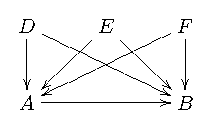
\includegraphics{pictures/covered_edge.eps}} \caption{Edge
$A\rightarrow B$ is covered, whereas $D\rightarrow A$ is not covered.}%
\label{fig:covered_arc}%
\end{figure}


\begin{theorem}  
  [Chickering-Meek]\label{lm:meek-conjecture}
  \label{thm:meek}
  Let $G$
and $H$ be two DAGs over the same set of variables $\mathbf{V}$. Then
$\D_{G}\subseteq\D_{H}\iff$ the DAG $H$ can be transformed
into the DAG $G$ by repeating the following two operations: (1)~covered edge
reversal, and (2)~single edge deletion.
\end{theorem}
%
The next corollary characterizes the
inclusion depth of a BN independence relation $\I_G$ for a graph $G$
in terms of a simple syntactic feature of $G$, namely the number of adjacencies in $\G$. For a BN dependence relation $\D_G$, the corresponding feature is the number of adjacencies {\em not} in $\G$.

%\begin{corollary}
\begin{proposition}
\label{cor:number-edges}Let $G = (\V,E)$ be a Bayes net structure. 
\begin{enumerate}
\item 
The inclusion depth of the BN-dependence relation
$\D_{G}$ equals ${\binom{|\mathbf{V}|}{2}} - |E|$, the number of adjacencies {\em not} in $G$.
%%, and we take the inclusion depth of a Bayes net to be the inclusion depth of its dependence relation. 
So the dependency relation defined by the totally
disconnected network has inclusion depth ${\binom{|\mathbf{V}|}{2}}$, and the dependency relation defined by the complete network has
inclusion depth $0$.  \label{depth-dependency}
\item \label{depth-independency} The inclusion depth of the BN-independency relation
$\I_{G}$ equals $|E|$, the number of adjacencies in $G$.
%%, and we take the inclusion depth of a Bayes net to be the inclusion depth of its dependence relation. 
So the independency relation defined by the totally
disconnected network has inclusion depth 0, and the independency relation defined by the complete network has inclusion depth ${\binom{|\mathbf{V}|}{2}}$.
\end{enumerate}
%\end{corollary}
\end{proposition}
\begin{proof}
  Part \ref{depth-independency} follows from Part \ref{depth-dependency}, since an inclusion chain $\D_{G_1} \subset \cdots \subset \D_{G_k}$ of BN-dependency relations corresponds to an inclusion chain $\I_{G_k} \subset \cdots \subset \I_{G_1}$ of the complementary independency relations. To establish Part \ref{depth-dependency}, we use downward induction on the number of edges $n$ in graph $G$. Let $N = {\binom{|\mathbf{V}|}{2}}$. 
  Base case: $n = N$. Then $G$ is a complete graph, so $\D_{G}$ contains all dependency statements in the statement space $\D_{\mathbf{V}}$, and therefore has 0 inclusion depth.
  Inductive step: Assume the hypothesis for $n+1$ and consider a graph $G$ with $n$ edges. 
  Add an edge to $G$ to obtain a BN $G'$ with $n+1$ edges that is a supergraph of $G'$. Adding an edge can only increase the number of d-connecting paths between two given variables, so $\D_{G} \subseteq \D_{G'}$. Suppose that the edge added is a new link between nodes $\A$ and $\B$ that are not adjacent in $\G$. By the d-separation Lemma \ref{lemma:d-sep},
there is a separating set $\S$
such that $\A,\B$ are d-separated by $\S$ in $\G$, that is, $(\A \indep \B|\S)_{\G}$. However in the graph $\G'$, the nodes $\A$ and $\B$ are adjacent, so they are not d-separated by any set, and we have $(\A \dep \B|\S)_{\G'}$. So $\G'$ entails strictly more dependencies than $\G$, that is,
$$\D_{G} \subset \D_{G'}.$$ By inductive hypothesis, there is an inclusion chain 
$$\D_{G'} \subset \D_{G_{1}} \cdots \subset \D_{G_{N-(n+1)}}$$
 consisting of BN dependency relations. Hence the inclusion depth of $G$ is at least $N - (n+1) + 1 = N - n$. 
  
To show that the inclusion depth of $G$ is exactly $N - n$, consider any inclusion chain
\begin{equation} \D_G \subset \D_{H} \subset \cdots \subset \D_{\mathbf{V}}.\label{eq:chain1} \end{equation} 
Theorem~\ref{thm:meek} implies that graph $\G$ can be obtained from $\H$ with covered arc reversals and/or edge deletions. If $\G$ can be obtained from $\H$ with covered arc reversals only, then $\H$ can be likewise obtained from $\G$, since covered edge reversals are symmetric, and so by Theorem~\ref{thm:meek} we would have $\D_{\G} = \D_{\H}$, contradicting the choice of $\H$. So $\H$ has at  least one more edge than $\G$ and thus $\H$ has at least $n+1$ edges. Applying the inductive hypothesis to $\H$, it follows that the inclusion chain 

$$\D_{H} \subset \cdots \subset \D_{\mathbf{V}}$$ 

has length at most $N-(n+1)$, so the inclusion chain (\ref{eq:chain1}) has at most $N - (n+1) + 1 = N - n$ members.
\end{proof}
%
Propositions \ref{prop:fin-thickness} and \ref{cor:number-edges} imply that
the mind change complexity of identifying a Bayes Net structure over variables
\textbf{V} %from dependency data 
is given by the maximum number of edges over
\textbf{V}.

\begin{corollary}
For any set of variables $\mathbf{V}$, the inclusion depth of $\L_{\mathbf{V}}^{\D}
$ and the inclusion depth of $\L_{\mathbf{V}}^{\I}
$ is ${\binom{|\mathbf{V}|}{2}}$. So the mind change complexity of identifying the
correct Bayes Net structure from dependency data or from independency data is ${\binom{|\mathbf{V}|}{2}}$.
\end{corollary}
%
The  next section characterizes the BN learning algorithms that achieve optimal mind change performance.

\section{Mind-Change Optimal Learners for Bayes Net Structure} \label{sec:learners}

%The complexity of a learning problem is a lower bound on the best possible
%performance by a learning algorithm. A goal of learning theory is to design
%algorithms that achieve the best possible performance. 
We analyze
mind-change optimal algorithms for identifying Bayes net structure. The
intuition underlying mind-change optimality is that a learner that is
efficient with respect to mind changes minimizes mind changes not only
globally in the entire learning problem, but also locally in subproblems after
receiving some evidence \cite{luo06:_mind_chang_effic_learn,luo05:_mind_chang_effic_learn,kelly04:_justif_truth_findin_effic}.
We
formalize this idea as in \cite[Def.2.3]{luo06:_mind_chang_effic_learn}. If a mind change
bound exists for $\L$ given $\sigma$, let $\MC_{\L%
}(\sigma)$ be the least $k$ such that $\L$ is identifiable with $k$
mind changes given $\sigma$. For example, given a sequence $\sigma$ of
dependencies, let $G=(\mathbf{V},E)$ be a BN that %covers (satisfies) 
satisfies
the
dependencies in $\sigma$ with a minimum number of edges. Then the mind change
complexity $\MC_{\L_{\mathbf{V}}^{\D}}(\sigma)$ is ${\binom{|\mathbf{V}|}{2}-|E|}$. Mind change optimality requires that a learner should succeed with $\MC_{\L}(\sigma)$ mind
changes after each data sequence $\sigma$. %\in\SEQ(\L)$.

\begin{definition}[based on Def.2.3 of \cite{luo06:_mind_chang_effic_learn}]
A learner $\Psi$ is \textbf{strongly mind-change optimal} (SMC-optimal) for
$\L$ if for all data sequences $\sigma$ the learner $\Psi$ identifies
$\L$ given $\sigma$ with at most $\MC_{\L}(\sigma)$ mind changes.
\end{definition}
%
The next proposition characterizes SMC-optimal learners for language
collections with finite inclusion depth. It follows from the general characterization of SMC-optimal
learners for all language collections established in \cite[Prop.4.1]{luo06:_mind_chang_effic_learn}.

\begin{proposition}
Let $\Psi$ be a learner that identifies a language collection $\L$
with finite inclusion depth. Then $\Psi$ is SMC-optimal for $\L$ if
and only if for all data sequences $\sigma$: if $\Psi(\sigma)\neq\,?$, then
$\Psi(\sigma)$ is the unique language consistent with $\sigma$ that maximizes inclusion depth.
% for
%$\sigma$.
\label{prop:char-smc}
\end{proposition}
%
Applying the proposition to Bayes net learners yields the following corollary.

\begin{corollary}
Let $\Psi$ be a Bayes net learner that identifies the correct Bayes net
pattern for a set of variables $\mathbf{V}$ from dependency data. The learner $\Psi$ is
SMC-optimal for $\lvd$ $\iff$ for all dependency sequences $\sigma$, if the output of
$\Psi$ is not ?, then $\Psi$ outputs %the 
a uniquely edge-minimal pattern for the
dependencies $\D=\content(\sigma)$.
\end{corollary}
%
It is easy to implement a slow SMC-optimal BN learner. For example, for a given set of dependencies $\D$ it is straightforward to check if there is a pattern $G$ that covers exactly those dependencies (i.e., $\D_G = \D$). So an SMC-optimal learner could output a pattern $G$ if there is one that matches the observed dependencies exactly, and output ? otherwise. But such a slow learner requires exponentially many dependency statements as input before it conjectures a graph. There are SMC-optimal learners that produce a guess faster; in fact, using Gold's notion of ``uniformly faster'', we can show that there is a  unique fastest SMC-optimal learner.
Gold proposed the following way to compare the convergence speed of two learners \cite[p. 462]{gold67limit}. %(we follow the notation of \cite[Def.8.1.C]{Osherson86}).

\begin{definition} \label{def:speed} Let $\L$ be a language collection.
\begin{enumerate}
\item The convergence time of a learner $\Psi$ on text $T$ is defined as
$\CONV(\Psi,T)\equiv$ the least time $m$ such that 
$\Psi(T[m])=\Psi(T[m'])$ for all $m'\geq m$.

\item A learner $\Psi$ identifies $\L$ uniformly
faster than learner $\Phi\iff$
\begin{enumerate}
\item for all languages $L\in\L$ and all texts $T$ for $L$, we have
$\CONV(\Psi,T)\leq \CONV(\Phi,T)$, and

\item for some language $L\in\L$ and some text $T$ for $L$, we have
$\CONV(\Psi,T)<\CONV(\Phi,T)$.
\end{enumerate}
\end{enumerate}
\end{definition}
%
For a language collection $\L$ with finite inclusion depth,
Proposition \ref{prop:char-smc} implies that if there is no language $L$ that
uniquely maximizes inclusion depth given $\sigma$, then a learner that is
SMC-optimal outputs $?$ on $\sigma$. Intuitively, the fastest SMC-optimal learner delays %procrastinates  
making a conjecture no longer than is necessary to meet this condition. 
Formally, this learner is defined as follows for
all sequences $\sigma\in \SEQ(\L)$:%
$$
\Psi_\fast^{\L}(\sigma)=
\begin{cases}
? & \text{if no language uniquely maximizes inclusion depth
given }\sigma\\
L & \text{if $L \in \L$ uniquely maximizes inclusion depth given $\sigma$.} 
\end{cases}
$$
The next observation asserts that $\Psi_\fast^{\L}$ is the fastest SMC-optimal method for a given language collection $\L$.

\begin{observation}
\label{obs:fastest}Let $\L$ be a language collection with finite
inclusion depth. Then $\Psi_\fast^{\L}$ is SMC-optimal and
identifies $\L$ uniformly faster than any other SMC-optimal learner
for $\L$.
\end{observation}

\begin{proof} 
%The proof is a variant of standard results on text-efficiency (e.g., \cite[Ch.2.3.3]{martin98elements}) and is omitted for space reasons.
It is easy to see that $\Psi_\fast^{\L}$ identifies
$\L$, so Proposition \ref{prop:char-smc} implies that $\Psi
_\fast^{\L}$ is SMC-optimal. 
Let $\Psi\neq\Psi_\fast^{\L}$
be any other SMC-optimal learner that identifies $\L$. %Again 
By Proposition \ref{prop:char-smc}, if $\Psi(\sigma)\neq\,?$, then $\Psi
(\sigma)=\Psi_\fast^{\L}(\sigma)$. So $\Psi$ does not converge faster than $\Psi_\fast^{\L}$ on any text. 
Therefore for any language $L\in
\L$ and text $T$ for $L$, we have \[
\CONV(\Psi_\fast^{\L%
},T)\leq \CONV(\Psi,T).
\] 
Let $\sigma\in \SEQ(\L)$ be a data
sequence such that $\Psi(\sigma)\neq\Psi_\fast^{\L}(\sigma) = L$. 
Since
both $\Psi$ and $\Psi_\fast^{\L}$ are SMC-optimal, 
 Proposition
\ref{prop:char-smc} implies that %there is a language 
$L$ %that
uniquely maximizes inclusion depth given $\sigma$. 
So $\Psi_\fast%
^{\L}(\sigma)=L$ and $\Psi(\sigma)=\,?$. Now let $T_{L}\supset\sigma$ be
any text for $L$ extending $\sigma$. 
It is easy to see that the language $L$ uniquely maximizes inclusion depth on any data sequence
$\sigma'$ with $\sigma\subseteq\sigma'\subset T_{L}$. So
\[
\CONV(\Psi_\fast^{\L},T_{L})\leq|\sigma|,
\] and %On the other hand, 
clearly 
\[\CONV(\Psi,T_{L})>|\sigma|\] since $\Psi(\sigma)=\, ?$.
 Thus $\Psi_\fast%
^{\L}$ identifies $\L$ uniformly faster than $\Psi$, and in
general faster than any other SMC-optimal learner.
\end{proof}

Observation \ref{obs:fastest} leads to the following algorithm for identifying a BN pattern from dependency data.

\begin{corollary} \label{cor:dep-learner}
Let $\mathbf{V}$ be a set of variables. For a given sequence of dependencies
$\sigma$, the learner $\Psi_\fast^{\D}$ outputs ? if there is more
than one edge-minimal pattern that covers the dependencies in $\sigma$, and
otherwise outputs 
a uniquely edge-minimal pattern for the
dependencies $\D=\content(\sigma)$. The learner $\Psi_\fast^{\D}$ is SMC-optimal and identifies the
correct pattern uniformly faster given dependency data than any other SMC-optimal BN structure learner.
\end{corollary}
%
The corollary shows that the criteria of mind-change optimality and convergence speed
determine a unique, natural and novel method for learning Bayes net structure. The next example illustrates this method.

% % Should we give an example of such a learner? This should
%% probably relate to previous examples.
\begin{example}
  Let $\mathbf{V}=\set{A,B,C,D}$. If
  \begin{align*}
    \sigma = (&B\dep D, B\dep D|\set{A},  B\dep D|\set{C},\\
   & C\dep D, C\dep D|\set{A}, C\dep D|\set{B},\\
   &B\dep C|\set{D}, B\dep C|\set{A,D}), 
 \end{align*}
  then $\Psi_{\fast}^{\mathbf{V}}$ outputs the graph shown in Figure~\ref{fig:output1}, for the following reasons. According to Corollary \ref{cor:dep-learner}, maximizing inclusion depth given dependency data is equivalent to minimizing the number of edges in the output graph. In any edge-minimal graph $\G$ consistent with the data $\sigma$, nodes $\B$ and $D$ are adjacent: if they are not adjacent in some graph $\G$, then by Lemma \ref{lemma:d-sep} there is a d-separating set $\S$ such that $(\B \indep D|\S)_{G}$. According to the data, $\B$ and $D$ are dependent given any proper subset of $\{\A,\C\}$, so we have $(\B \indep D|\{\A,\C\})_{G}$. The skeleton of any such graph $\G'$ must contain undirected paths $\B - \A - D$ and $\B - \C - D$, that is, all paths between $\B$ and $D$ are blocked by $\A$ and $\C$, but there is an unblocked path given just $\A$ and an unblocked path given just $\C$. But any such graph $\G$ contains 4 edges, whereas the graph shown in Figure~\ref{fig:output1} entails the dependencies in $\sigma$ with just two edges. So nodes $\B$ and $D$ are adjacent in any edge-minimal graph consistent with $\sigma$. The same argument holds for nodes $\C$ and $D$, so any edge-minimal graph consistent with $\sigma$ contains a triple $\B-D-\C$. To entail the observed dependence $B\dep C|\set{D}$, that triple must be oriented as $\B \rightarrow D \leftarrow \C$; the only alternative is to add an edge between $\B$ and $\C$, but this fails to minimize the number of edges. So the only pattern with only two edges that is consistent with the observed dependencies $\sigma$ is the one shown in Figure~\ref{fig:output1}. 
  
  Now suppose after some time, we have accumulated more data, and obtain the following data sequence
  \begin{align*}
    \sigma' = \sigma & \cup\\
&A\dep B, A\dep B|\set{C}, A\dep B|\set{D},\\
&A\dep C, A\dep C|\set{B}, A\dep C|\set{D}, B\dep C ),
%    \sigma' = (&B\dep D, B\dep D|\set{A},  B\dep D|\set{C},\\
%&    C\dep D, C\dep D|\set{A}, C\dep D|\set{B},\\
%&    B\dep C|\set{D}, B\dep C|\set{A,D},\\
%&A\dep B, A\dep B|\set{C}, A\dep B|\set{D},\\
%&A\dep C, A\dep C|\set{B}, A\dep C|\set{D}, B\dep C ),
  \end{align*}
 then the optimal learner $\Psi_{\fast}^{\mathbf{V}}$ outputs the graph shown in Figure~\ref{fig:output2}, for the following reasons. Similar to the analysis of the previous data, any edge-minimal graph must have $\A$ adjacent to $\B$: For if $\A$ is not adjacent to $\B$ in a graph $\G$ consistent with $\sigma'$, then the skeleton of $\G$ must contain two paths $\A - \C - \B$ and $\A - D - \B$, and if $\G$ has the minimum number of 4 necessary edges, these are all the links in $\G$. In any DAG with such a skeleton, there is at least one collider (else a cycle would occur). Suppose without loss of generality that $\B$ is a collider, so the graph contains a triple $\C \rightarrow \B \leftarrow D$. But then either the dependence $\C \dep D|\A$ or the dependence $\C \dep D$ is not entailed by $\G$. So any graph with only 4 edges that is consistent with $\sigma'$ has the same skeleton as that shown in Figure~\ref{fig:output2}. The only remaining question is the placement of colliders. If both $\A$ and $D$ are colliders, the dependence $\B \dep \C$ fails. If neither is a collider, the dependence $\B \dep \C|\{\A,D\}$ fails. If $\A$ is a collider and $D$ is not, the dependence $\B \dep \C|\{D\}$ fails. So the only possibility is to have $D$ as a collider and $\A$ not a collider, which results in the pattern shown in Figure~\ref{fig:output2}.
  \begin{figure}[h]
    \centering
    \subfigure[]{
      \label{fig:output1}
      \scalebox{0.4}{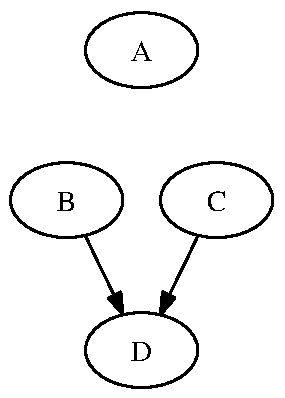
\includegraphics{pictures/output1}}
    }
    \hspace{3cm}
    \subfigure[]{
      \label{fig:output2}
      \scalebox{0.4}{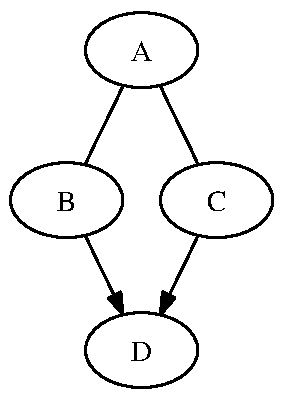
\includegraphics{pictures/output2}}
    }

    \caption{To illustrate SMC-optimal learning from dependency data. (a) The output of the optimal learner $\Psi_{\fast}^{\mathbf{V}}$ on example data $\sigma$. (b)The output of the optimal learner $\Psi_{\fast}^{\mathbf{V}}$ on example data $\sigma'$.}
    \label{fig:outputs}
  \end{figure}
\end{example}
%
The next corollary characterizes the fastest mind-change optimal learner for independency data.

\begin{corollary}
Let $\mathbf{V}$ be a set of variables. For a given sequence of independencies
$\sigma$, the learner $\Psi_\fast^{\I}$ outputs ? if there is more
than one edge-maximal pattern that covers the independencies in $\sigma$, and
otherwise outputs 
a uniquely edge-maximal pattern for the
independencies $\I=\content(\sigma)$. The learner $\Psi_\fast^{\I}$ is SMC-optimal and identifies the
correct pattern uniformly faster given independency data than any other SMC-optimal BN structure learner.
\end{corollary}
%
Intuitively, the learner $\Psi_\fast^{\I}$ removes as many potential adjacencies as are necessary to entail the independencies given in the data. One of the most prominent constraint-based algorithms, the PC algorithm \cite[Ch.5.4.2]{peter00:_causat}, can be seen as a heuristic implementation of this idea: Basically, the PC algorithm starts with the completely connected network over $n$ variables, and then successively considers independencies of the form $\X\protect{\indep} \Y|\S$, for $|\S|=0,1,\ldots,n$, removing links between the conditionally independent variables $X$ and $Y$. Examples of the kind of Bayes net structure that result from this algorithm are given in \cite{peter00:_causat}.
The remainder of the paper analyzes the run-time complexity of the optimal $\Psi_\fast^{\D}$ and $\Psi_\fast^{\I}$ methods; we show that computing the output
of these learners is $\NP$-hard (assuming that $\Poly=\RP$). The proof gives two many-one reductions of the problem of deciding the existence of a unique
exact cover by 3-sets, to the problems of computing the output of the fastest mind
change optimal learner from independency respectively dependency data.

 
\section{Computational Complexity of Fast Mind-Change Optimal Identification of Bayes Net Structure from Independency Data}  \label{sec:complexity}

Because the $\NP$-hardness proofs for the optimal learners are quite different for dependency and independency data, we divide the analysis into different sections. We begin with the setting of independency data, whose $\NP$-hardness proof is much simpler. General complexity theory concepts and notation were reviewed in Section \ref{sec:complexity-back}.

We describe the standard approach of analyzing the complexity of constraint-based learners in the Bayes net literature. 
As with any run-time analysis, an important issue is the representation of the input to the algorithm. The most straightforward approach for our learning model would be to take the input as a list of (in)dependencies, and the input size to be the size of that list. However, in practice CB learners do not receive an explicitly enumerated list of (in)dependencies, but rather they have access to a statistical oracle (cf. Section \ref{sec:discuss-model}). Enumerating relevant (in)dependencies through repeated queries to the oracle is part of the computational task of a CB learner. Accordingly, the standard complexity analysis takes an (in)dependency oracle and a set of variables as the input to the learning algorithm (e.g., \cite[Def.12]{chickering04:_large_sampl_learn_bayes_networ_np_hard},\cite{bouckaert95:_bayes}). The oracle is assumed to be represented syntactically in a reasonably concise way. For example, it may be a Turing Machine that computes the characteristic function of a given dependency relation $\D$.  
%To facilitate comparison with the related literature, 
%we follow the approach of representing the set of dependencies in the data through an oracle. We remark that the $\NP$-hardness result for the learner $\Psi_{\fast}^{\mathbf{V}}$ still holds if the input are enumerated dependencies (see below).

\begin{definition}
  An independency oracle $O$ for a variable set $\mathbf{V}$
  is a function that takes as input independency queries
  from the independency space $\I_{\mathbf{V}}$ and returns, in constant time, either ``yes'' or ``?''.
\end{definition}
%
The independency relation associated with oracle $O$ is given by
$\I_O = \{X \dep Y |\mathbf{S} \in \I_{\mathbf{V}}:
O \linebreak[0]\mbox{ returns} \linebreak[0] \text{ ``yes'' on input }\linebreak[0]X \indep Y |\mathbf{S}\}$. The oracle represents the independencies observed on a finite data sample, which may be incomplete; that is, there need not be any graph $\G$ such that $\I_{\G} = \I_{O}$.

%The notion of a one-sided dependency oracle makes clear the relationship to the standard CB learning model, which presupposed the existence of a two-sided oracle: (1) a dependency oracle assumes valid statistical testing only for dependence findings, not independence conclusions, and (2) our sequential data model envisions the dependency model becoming more informative as more data is obtained, whereas the standard model considers a completely informative oracle at a single point in time.

{\em Remark.} Our model of learning Bayes net structure can be reformulated in terms of a sequence of oracles: Instead of a complete sequence of independence statements for an independence relation $\I_G$, the learner could be presented with a sequence of independency oracles
$O_1,O_2,\ldots,O_n,\ldots$ such that $\I_{O_i} \subseteq \I_{O_{i+1}}$ and $\bigcup_{i=1}^{\infty} \I_{O_i} = \I_G$. 
The mind change and convergence time results remain the same in the independency oracle model.

We say that a pattern $\G$ is an {\bf I-cover} of a set of independencies $\I$ if $\G$ entails all the independencies in $\I$ (i.e., $\I \subseteq \I_{\G}$).
Computing the conjectures of the 
%fastest SMC-optimal 
learner $\Psi^{\I}_{\fast}$ poses the following computational problem.
%which we label \textsc{Unique Minimal I-map}.


\begin{description}
\item[\textsc{Unique Maximal I-cover}]
\item[Input] A set of variables \textbf{V} and an independency oracle $O$
for \textbf{V}.
\item[Output] If there is a \emph{unique} DAG pattern $G$ that entails the
independencies in $O$ with a maximal number of edges, output $G$. Otherwise
output ?.
\end{description}
%\end{definition}
This is a function maximization problem; the corresponding decision problem is the following.%\textsc{Unique I-map} problem.
\begin{description}
\item[\textsc{Unique I-cover} ]
\item[Instance] A set of variables \textbf{V}, an independency oracle $O$
for \textbf{V}, and a bound $k$.
\item[Question] Is there a DAG pattern $G$ such that: $G$ entails the
  independencies in $O$, every other DAG pattern $G'$
  entailing the independencies in
  $O$ has fewer edges than $G$,
  and $G$ has at least $k$ edges?
\end{description}
%\end{definition}
%
Clearly an efficient algorithm for the function maximization problem yields an
efficient algorithm for \textsc{Unique I-cover}. We will
show that \textsc{UEC3SET} reduces to \textsc{Unique I-cover}. We also give an upper bound on the problem complexity in terms of oracle computations. Recall that \textsc{SAT} is the $\NP$-complete satisfiability problem and $\FP^{(\NP^{\NP})}$ is the class of functions computable in polynomial time given an oracle for decision problems in $\NP^{\NP}$.


\begin{theorem} \label{theo:complex-indep} The computational complexity of \textsc{Unique Maximal I-cover}. 

\begin{enumerate}
\item \textsc{Unique Maximal
I-cover} is in $\FP^{(\NP^{\NP})}$. \label{clause:upper-indep}
\item $\textsc{SAT} \leq_{\RP} \textsc{UEC3SET} \leq_{\Poly} \textsc{Unique I-cover} \leq_{\Poly} \textsc{Unique Maximal I-cover}$. So \textsc{Unique Maximal
I-cover} is $\NP$-hard provided that $\Poly=\RP$. \label{clause:np-hard-indep}
\end{enumerate}

\end{theorem}
\begin{proof}
Part \ref{clause:upper-indep}: 
We specify a program that computes the output of the fastest SMC-optimal learner $\Psi^{\I}_{\fast}$ given a set of $n$ input nodes, an independency oracle $O$, and an oracle for computational problems in ${\NP}^{\NP}$. A pattern $\G$ is an I-cover of $O$ just in case the answer to the question ``is there a dependency $\X \indep \Y|\S$ such that $\X \indep \Y|\S \in (I_{O} - I_{\G})$'' is no. So an oracle for $\NP$ decides in constant time whether a pattern $\G$ is an I-cover of $O$.
\begin{enumerate}
\item Find the maximum number of edges $k$, for $k=1,\ldots,\binom{n}{2}$, such that there is a pattern $\G$ that is an I-cover of $\O$. Given an $\NP$-oracle for deciding whether $\G$ is an I-cover of $\O$, for a given $k$ this query can be answered in polynomial time with a nondeterministic computation. Using binary search, this step therefore can be carried out with $O(log(n))$ queries to the ${\NP}^{\NP}$ oracle. 
\item Having determined the maximum number $k$ of edges, ask ``are there two distinct patterns $\G,\G'$ such that both $\G$ and $\G'$ are I-covers of $O$ and $\G$ and $\G'$ contain $k$ edges{?}''. Given an $\NP$-oracle for deciding whether $\G$ and $\G'$ are I-covers of $\O$, this query can be answered in polynomial time with a nondeterministic computation, hence with a single query to the ${\NP}^{\NP}$ oracle. If the answer is ``yes'', output ?, since there is no unique I-cover with a maximum number of edges. If the answer is ``no'', there is a unique I-cover with a maximum number of edges; continue to the next step.
\item Using a standard method, construct an output pattern $\R$ as follows. For each pair of nodes $\X,\Y$ and each of the possible link types $\X-\Y, \X \rightarrow\Y, \X \leftarrow \Y$, ask ``is there a pattern $\G$ with $k$ edges that contains the given link type between $\X$ and $\Y$ and is an I-cover of $I_{O}$''. As in the previous step, this query can be answered in constant time with an ${\NP}^{\NP}$ oracle for a given pair of nodes $\X,\Y$ and type of link between them. Since the edge-maximizing I-cover is unique, the answer is ``yes'', for at most one of these link types. If the test indicates a link of a certain type between $\X$ and $\Y$, add the link to $\R$. This requires $O(\binom{n}{2})$ queries to the ${\NP}^{\NP}$ oracle. 
\end{enumerate}
This procedure returns the output of the fastest SMC-optimal learner $\Psi^{\I}_{\fast}$ with total runtime bounded by $O(\binom{n}{2})$.

Part \ref{clause:np-hard-indep}:
We give a reduction from \textsc{unique X3Set} to \textsc{Unique I-Cover
with At Least k edges}. Consider an instance of \textsc{UEC3SET} with sets
universe $U$ of size $|U|=3m$, and $c_{1},\ldots,c_{p}$, where $|c_{i}|=3$ for
$i=1,\ldots,p$ and $U=\cup_{i=1}^{m}c_{i}$. Define the following set $\V$ of variables.

\begin{enumerate}
\item For every set $c_{i}$, a {\em set variable} $C_{i}$.

%\item For every element $x_{j}$ of the universe $U$, a {\em member variable} $X%
%_{j}$.

\item A {\em root variable} $R$.
\end{enumerate}
We write $\x$ for the element corresponding to node $\X$, and similarly $\c$ for the set corresponding to node $\C$. 
Set the bound $k=m$. The following program implements an
independency oracle $O$ over the variables $\V$, in time polynomial in the size of the given \textsc{UEC3SET} instance.

\begin{description}
\item[Definition of Independency Oracle]
\item[Input] An independency query $V_1 \indep V_2 | \S$.

\item[Output] Oracle Clauses

\begin{enumerate}
%\item If $V_{1}=\X_{i},V_{2}=\X_{j}%
%,\S\mathbf{=\emptyset},$ then return ``independent". \label{clause:noedge-members}
%\item If
%$V_{1}=\C_{i},V_{2}=\X_{j},\S = \emptyset$, and $x_{j}\notin c_{i}$, then
%return ``independent". \label{clause:noedge-wrongset}
%\item If $V_{1}=\X_{i},V_{2}=R$, and $\S=\{\C_{j}:x_{i}\in c_{j}\}$, then return
%``independent". \label{clause:noedge-memberroot}
\item If $V_{1}=\C_{i},V_{2}=\C
_{j}$, and $\S=\emptyset$, then return ``independent". \label{clause:noedge-sets}
\item If $V_{1}=\C_{i},V_{2}=\C_{j},\S=\{\R\}$ and $\c_i \cap \c_j \neq \emptyset$, then return ``independent". \label{clause:colliders}
\item In all other cases, return ?.
\end{enumerate}

\end{description}
We use the terms adjacency, edge, and link interchangeably.
Let $\I_O$ be the set of independencies associated with oracle $O$. We argue that every I-cover for $\I_O$ with at least $m$ adjacencies corresponds to an exact set cover for the given instance of  \textsc{UEC3SET}, and vice versa. 

Suppose that $\G$ is an I-cover for $\I_O$ with at least $m$ adjacencies. Clause \ref{clause:noedge-sets} implies that all adjacencies are of the form $\C - \R$: the only other possibility is an adjacency $\C-\C'$ between set variables, but then $\C$ and $\C'$ are d-connected in $\G$ given the empty set, whereas Clause \ref{clause:noedge-sets} requires that they be d-separated given the empty set.
The case with $m=1$ is trivial; for $m > 1$, Clause \ref{clause:noedge-sets} implies that the adjacencies are directed as $\C \rightarrow \R$: for suppose otherwise. Then there is a link of the form $\C \leftarrow \R$. Since $m > 1$, there is at least one other link $\C' - \R$ with $\C \neq \C'$. Now $\R$ is not a collider on the path $\C \leftarrow \R - C'$, so $\C$ and $\C'$ are d-connected in $\G$ given the empty set, whereas Clause \ref{clause:noedge-sets} requires that they be d-separated given the empty set. Given that $\R$ is therefore a collider on any path $\C - \R - \C'$, it follows that $\C \dep \C'| \{R\}$ whenever $\C,\C'$ are neighbors of $\R$. The contrapositive of Clause \ref{clause:colliders} says that if $\C \dep \C'|\{\R\}$, then $\c \cap \c' = \emptyset$. Thus the neighbors of $\R$ correspond to mutually disjoint sets, so there are exactly $m$ neighbors of $\R$ forming an exact set cover. 

Conversely, it is easy to see that if the collection $\{\c^1,\ldots,\c^m\}$ forms an exact cover of the universe $\U$, then the graph containing all edges $\C^i \rightarrow \R$, for $i=1,\ldots,m$, is an I-cover of $\I_O$. So there is a 1-1 onto mapping between I-covers of $\I_O$ with at least $m$ edges and exact set covers for the given set cover instance. Hence there is a unique I-cover of $\I_O$ with at least $m$ edges if and only if there is a unique exact set cover.
\end{proof}

The gap between our upper and lower bounds is typical for problems in the higher levels of the polynomial hierarchy, where both lower bounds and completeness in a class are difficult to establish (see \cite[Ch.17]{papadimitriou94:_comput}, especially the discussion of the Minimum Circuit problem, and \cite[Ch.5]{Rothe2005}, especially the discussion of \textsc{Unique SAT}). 

The next section establishes a corresponding upper and lower bound for the problem of computing the output of the fastest SMC-optimal learner from dependency data, which requires a much more difficult construction for the lower bound. The reason why the hardness proof for dependency data is much more complex than for independency data is that there are many ways to achieve d-connection between two variables $\A$ and $\B$, whereas d-separation immediately entails the absence of a link between $\A$ and $\B$.


\section{Computational Complexity of Fast Mind-Change Optimal Identification of Bayes Net Structure from Dependency Data}

The definitions for the complexity analysis for dependency data parallel those for independency data. 


\begin{definition}
  A dependency oracle $O$ for a variable set $\mathbf{V}$
  is a function that takes as input dependency queries
  from the dependency space $\D_{\mathbf{V}}$ and returns, in constant time, either ``yes'' or ``?''.
\end{definition}
%
The dependency relation associated with oracle $O$ is given by
$\D_O = \{X \dep Y |\mathbf{S} \in \D_{\mathbf{V}}:
O \linebreak[0]\mbox{ returns} \linebreak[0] \text{ ``yes'' on input }\linebreak[0]X \dep Y |\mathbf{S}\}$. The oracle represents the dependencies observed on a finite data sample, which may be incomplete; that is, there need not be any graph $\G$ such that $\D_{\G} = \D_{O}$. As with independency data, our model of learning Bayes net structure can be reformulated in terms of a sequence of dependency oracles, where instead of a complete sequence of dependence statements, the learner is presented with a sequence of dependency oracles converging to the target independency relation. The mind change and convergence time results remain the same in the dependency oracle model.

A pattern $\G$ is an \textbf{I-map} of a set of dependencies $\D$ if $\G$ entails all the dependencies in $\D$ (i.e., $\D \subseteq \D_{\G}$, cf. \cite{pearl88:_probab_reason_intel_system}).
Computing the conjectures of the 
%fastest SMC-optimal 
learner $\Psi^{\D}_{\fast}$ poses the following computational problem. %which we 

\begin{description}
\item[\textsc{Unique Minimal I-map}]
\item[Input] A set of variables \textbf{V } and a dependency oracle $O$
for \textbf{V}.
\item[Output] If there is a \emph{unique} DAG pattern $G$ that entails the
dependencies in $O$ with a minimal number of edges, output $G$. Otherwise
output ?.
\end{description}
%\end{definition}
 The corresponding decision problem is the following.%\textsc{Unique I-map} problem.
\begin{description}
\item[\textsc{Unique I-map} ]
\item[Instance] A set of variables \textbf{V}, a dependency oracle $O$
for \textbf{V}, and a bound $k$.
\item[Question] Is there a DAG pattern $G$ such that: $G$ covers the
  dependencies in $O$, every other DAG pattern $G'$
  entailing the dependencies in
  $O$ has more edges than $G$,
  and $G$ has at most $k$ edges?
\end{description}
%\end{definition}
Clearly an efficient algorithm for the function minimization problem yields an
efficient algorithm for \textsc{Unique I-map}. We will
show that \textsc{UEC3SET} reduces to \textsc{Unique I-map}. We also give an upper bound on the problem complexity in terms of oracle computations.

\begin{theorem} The computational complexity of \textsc{Unique Minimal
I-map}. 
\begin{enumerate}
\item \textsc{Unique Minimal
I-map} is in $\FP^{(\NP^{\NP})}$. \label{clause:upper-dep}
\item $\textsc{SAT} \leq_{\RP} \textsc{UEC3SET} \leq_{\Poly} \textsc{Unique I-map} \leq_{\Poly} \textsc{Unique Minimal I-map}$. So \textsc{Unique Minimal
I-map} is $\NP$-hard provided that $\Poly=\RP$. \label{clause:np-hard-dep}
\end{enumerate}
\end{theorem}

\textbf{Proof.} Part \ref{clause:upper-dep} can be proven like Theorem \ref{theo:complex-indep}(\ref{clause:upper-indep}). 
For Part \ref{clause:np-hard-dep}, we give a reduction from \textsc{UEC3SET} to \textsc{Unique I-map}. Consider an instance of \textsc{UEC3SET} with sets
universe $U$ of size $|U|=3m$, and $c_{1},\ldots,c_{p}$, where $|c_{i}|=3$ for
$i=1,\ldots,p$ and $U=\cup_{i=1}^{m}c_{i}$. Define the following set $\V$ of variables.

\begin{enumerate}
\item For every set $c_{i}$, a {\em set variable} $C_{i}$.

\item For every element $x_{j}$ of the universe $U$, a {\em member variable} $X%
_{j}$.

\item A {\em root variable} $R$.
\end{enumerate}

We write $\x$ for the element corresponding to node $\X$, and similarly $\c$ for the set corresponding to node $\C$. 
Set the bound $k=3p+m$. The following program $M$ implements a dependency
oracle $O$ over the variables $V$, in time polynomial in the size of the given \textsc{UEC3SET} instance.

\begin{description}
\item[Definition of Dependency Oracle]
\item[Input] A dependency query $V_1 \dep V_2 | \S$.

\item[Output] Oracle Clauses
\begin{enumerate}
\item If $V_{1}=C_{i},V_{2}=X_{j}$, and $x_{j}\in c_{i}$, then return
``dependent''. \label{set}
\item If $V_{1}=X_{i},V_{2}=X_{j}$,
and there is a set $c_{k}\supseteq\{x_{i},x_{j}\}$ such that $C_{k}\in \S$, then return ``dependent''. \label{member}
\item If $V_{1}= R,V_{2}=X_{j},\S = \emptyset$ then return ``dependent''. \label{emptyset}
\item If $V_{1}= R,V_{2}=X_{j}, |\S| = 1$, and $\S \neq \{C\}$ where $x_j \in c$, then return ``dependent''. \label{clause:single}
\item In all other cases, return ?.
\end{enumerate}
\end{description}
We argue that there is a unique exact set cover for an instance $\langle
U,\{c_{i}\}\rangle$ iff there is a unique I-map with at most $k$ edges for $O$. 
So if there were a polynomial time algorithm $A$ for \textsc{Unique I-map}, we could solve the \textsc{UEC3SET} instance in polynomial time by using the program $M$ to ``simulate'' the oracle $O$ and use $A$ to solve the corresponding instance of \textsc{Unique I-map}. 
Our proof strategy is as follows. Consider what we refer to as the {\em basic graph} for $O$, shown in Figure \ref{fig:basic}. 
The basic graph is
also a pattern because all arrows correspond to unshielded colliders. 
\begin{figure}[htbp] %  figure placement: here, top, bottom, or page
   \centering
   %\scalebox{0.6}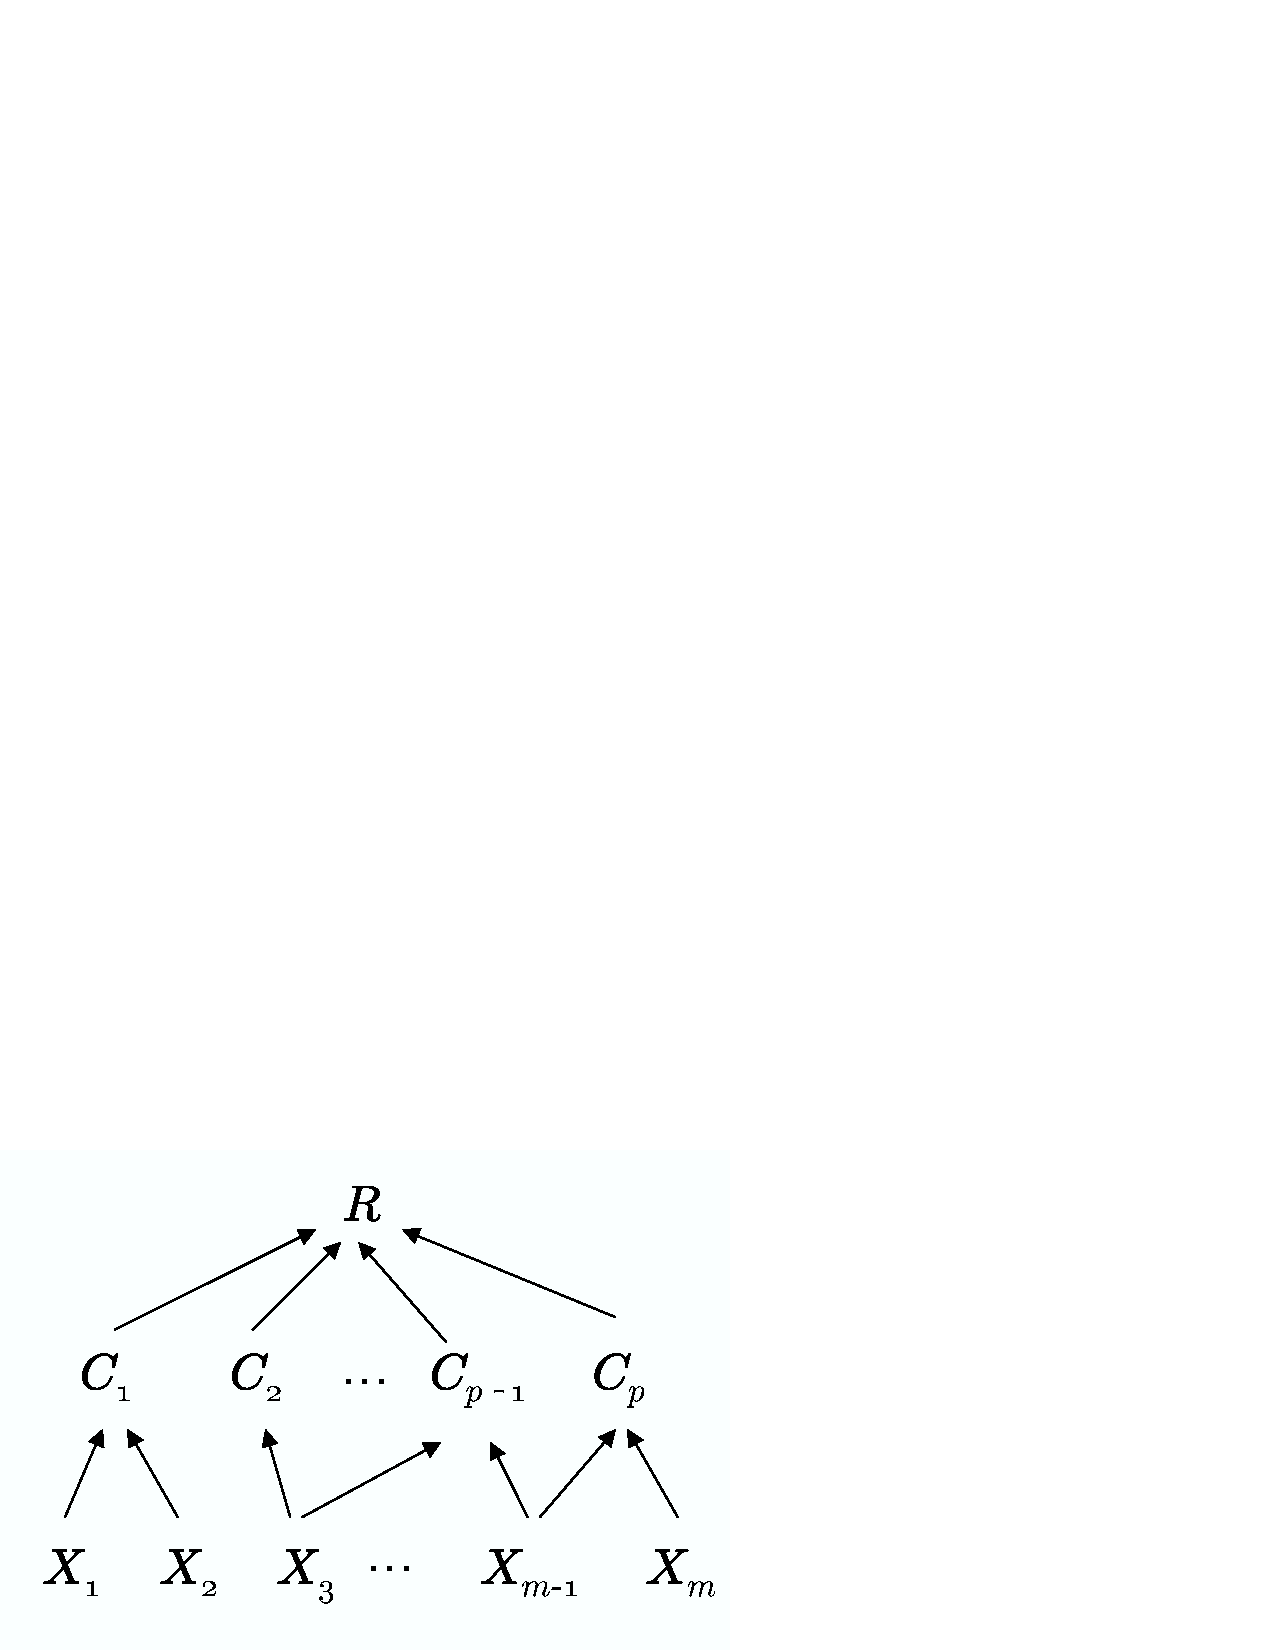
\includegraphics{pictures/target}
   % 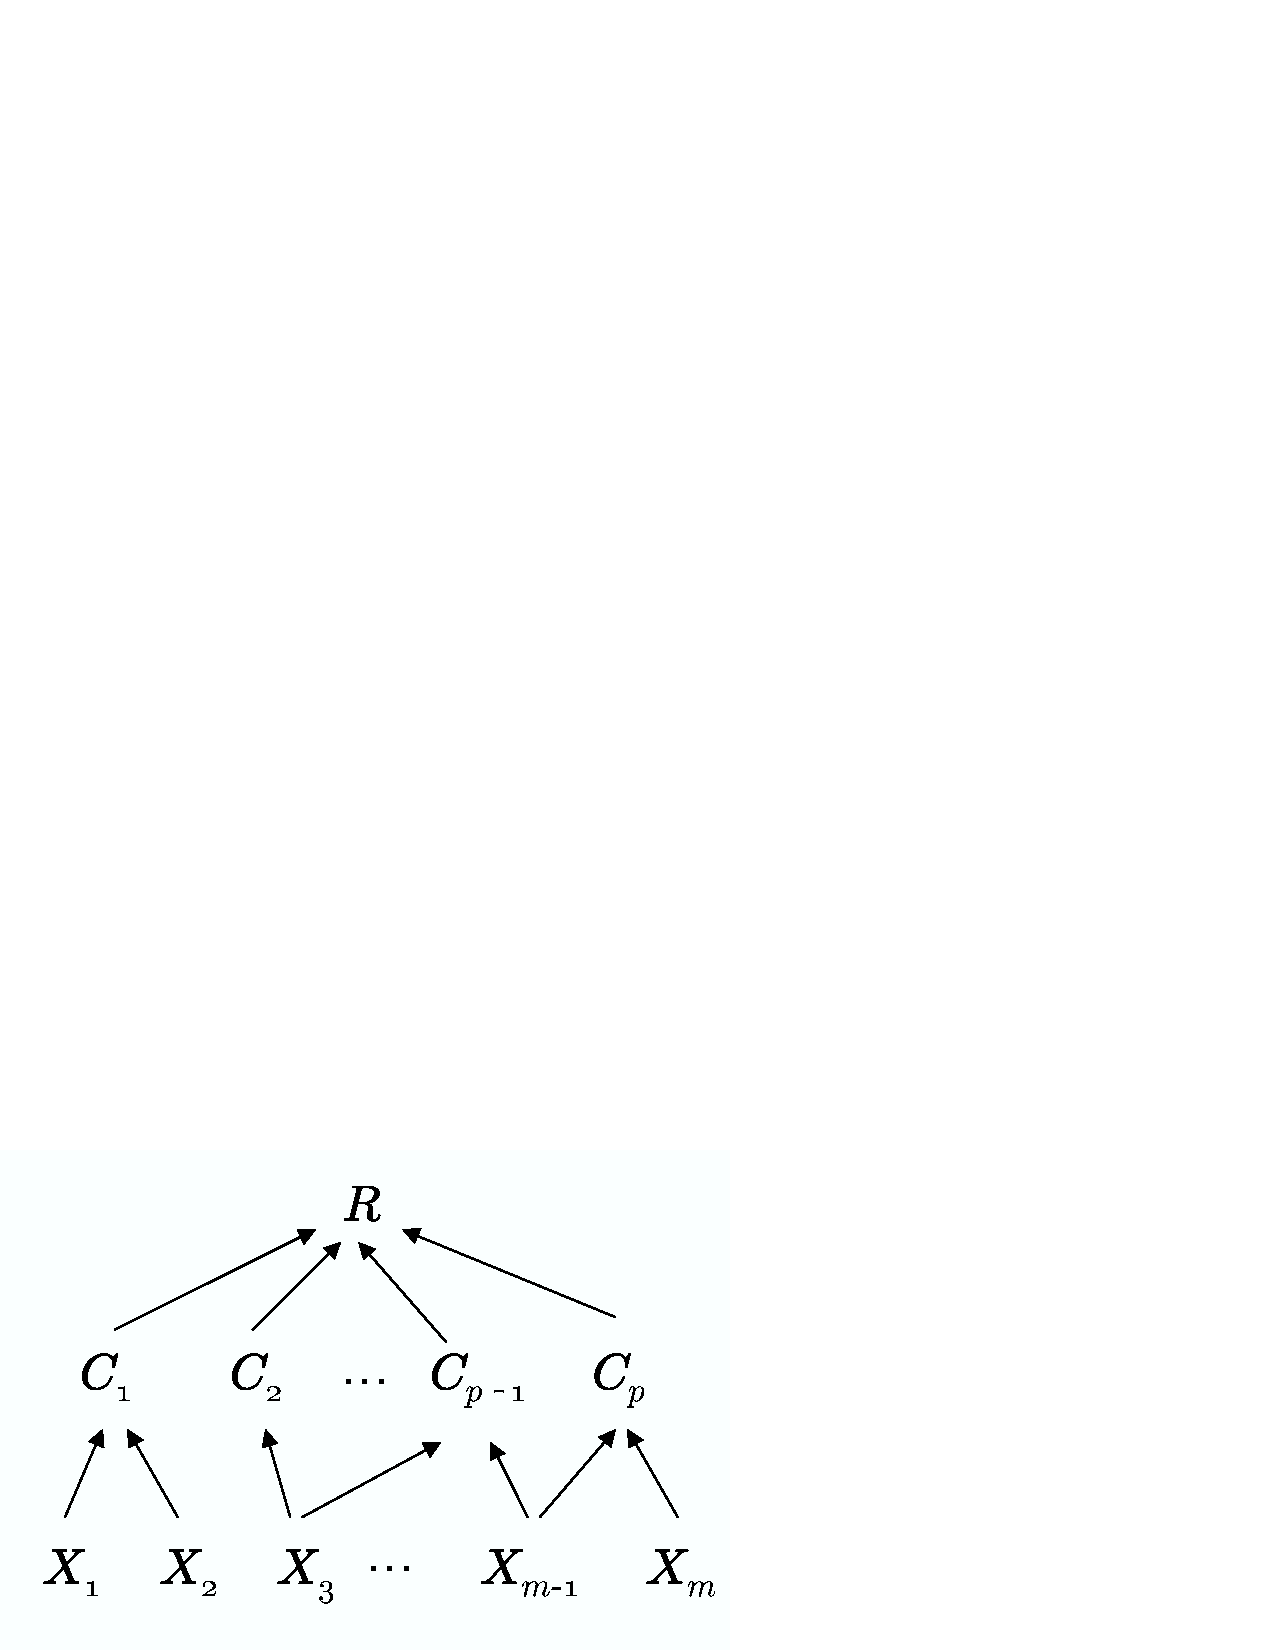
\includegraphics[width=1.8in]{pictures/target}
   \scalebox{0.4}{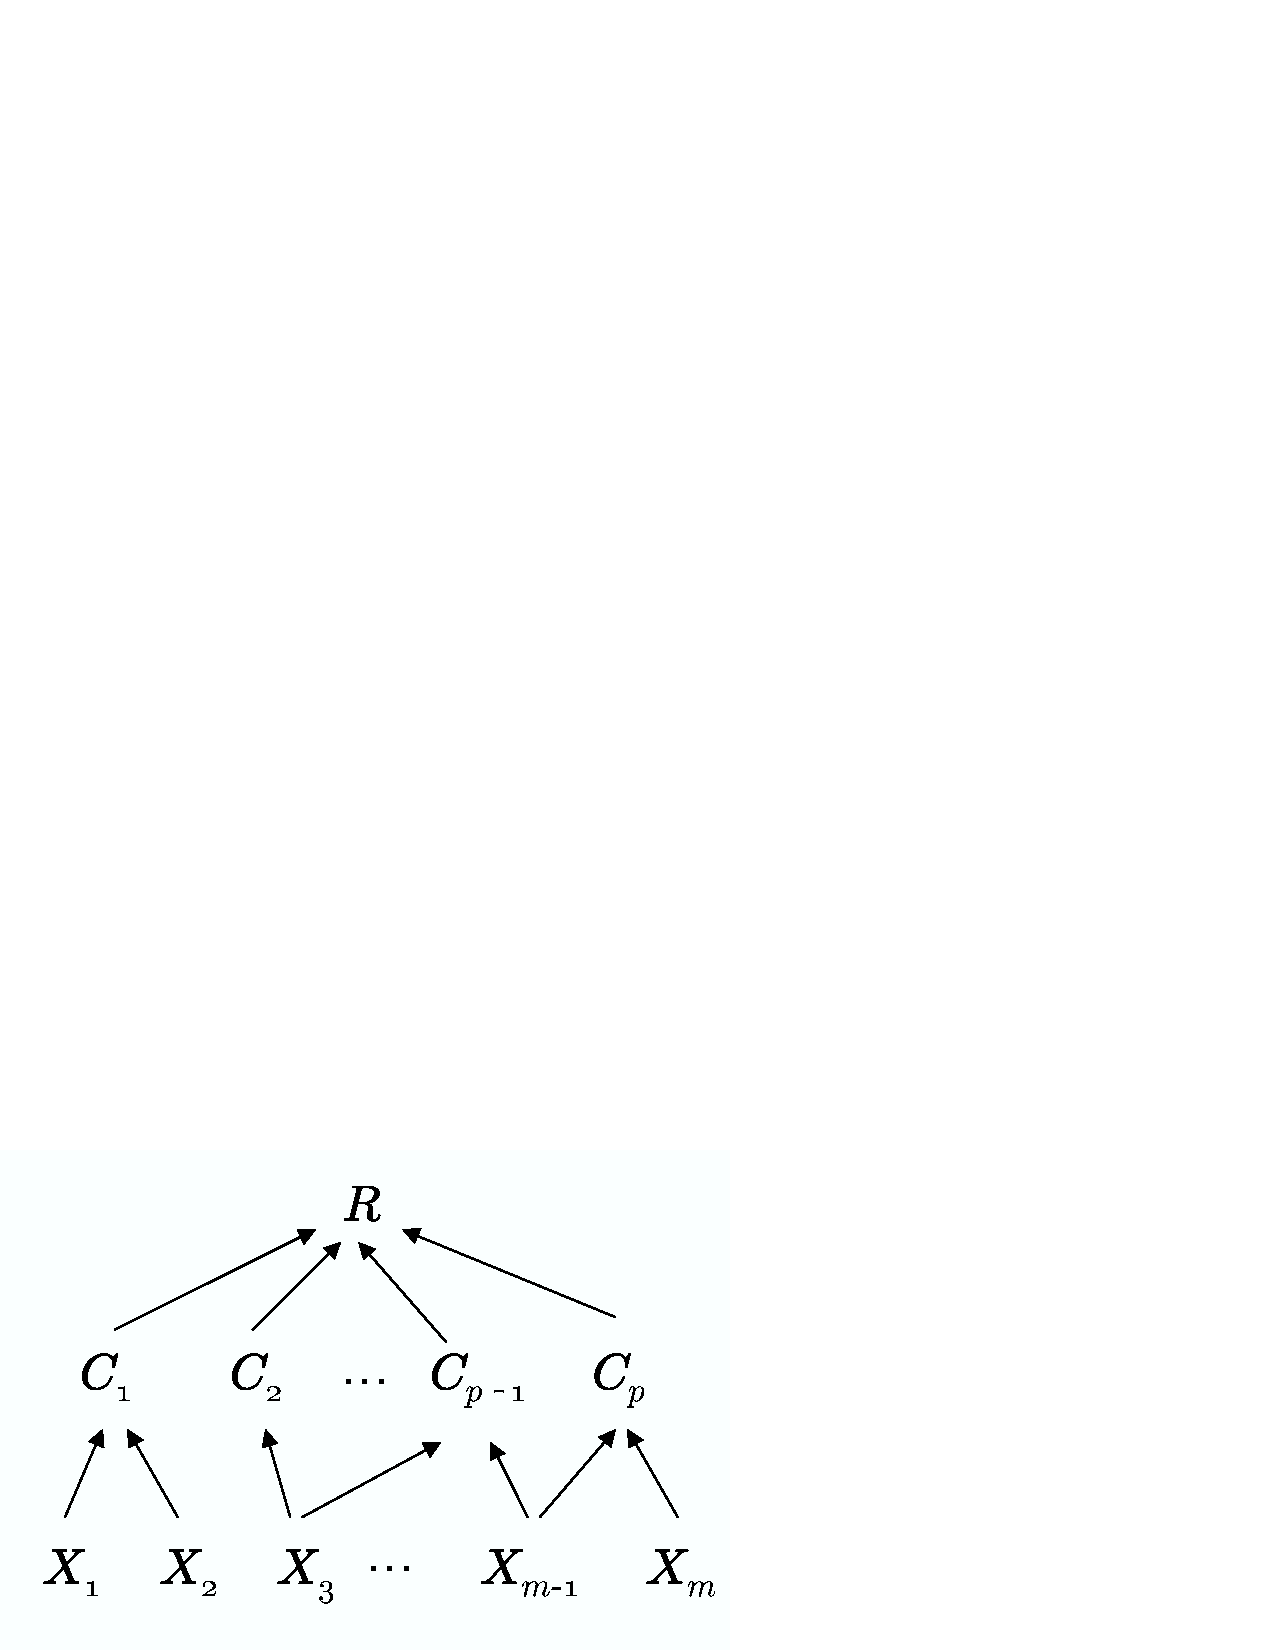
\includegraphics{pictures/target}}
   \caption{The basic graph for the $\NP$-hardness proof.
     A set cover of size $m$ corresponds to $m$ edges of the form $C \rightarrow R$.}
   \label{fig:basic}
\end{figure}
We show
that if there is a unique I-map $G$ for $O$ with at most $k$ edges, then $G$ is a subgraph
of the basic graph, with possibly edges $C_{i}\rightarrow R$
missing for some sets $c_{i}$, such that the set of variables $\{C_{1},C_{2},\ldots,C_m\}$ with the edge $C%
_{i}\rightarrow R$ in $G$ corresponds to an exact cover $\{c_{1},\ldots,c_{m}%
\}$. Conversely, any unique exact cover corresponds to a subgraph of the basic
graph in the same manner. %For reasons of space, we just illustrate most of the following assertions rather than giving full proofs.

In the following arguments we use the terms adjacency, edge, and link interchangeably.
For notation, we use an undirected link as in $\A - \B$ to indicate that nodes $\A$ and $\B$ are adjacent in a given graph, but the direction of the link is not determined by the context. The notation $\A - \cdots -\B$ indicates a path starting with $\A$ and ending in $\B$ where the direction of the links involving $\A$ and $\B$ is not determined. The notation $\A - \cdots \rightarrow \B$ indicates that  the last edge points into $\B$, etc. 
It is easiest to consider separately the constraints
imposed by each clause of $O$. Let $\D_i$ be the {\em set of dependencies corresponding to Clause $i$.} For example, $D_{\ref{set}} = \{\langle C_i, X_j, \S \rangle: x_j \in c_i\}$. 
%For example, $D_{\ref{emptyset}} = \{\langle X_j \dep R|\emptyset \rangle: j = 1,\ldots,3m\}$. 
The implications of $\D_{\ref{set}}$ are as follows.

% \emph{(1) Let graph }$G$\emph{\ be an I-map for }$\D_{\ref{set}}$\emph{. Then any two
% variables }$X$\emph{\ and }$C$\emph{\ are adjacent whenever
% }$ x \in c$\emph{.}
\begin{assertion} \label{ass:adjacency}
Let DAG $G$ be an I-map for $\D_{\ref{set}}$. Then any two
%variables 
nodes $X$ and $C$ are adjacent whenever
$ x \in c$.
\end{assertion}
\begin{proof} The d-separation lemma \ref{lemma:d-sep} implies that if
$G$ entails the dependencies in $\D_{\ref{set}}$, then $x$ and $C$ are adjacent
whenever $x \in c$. \end{proof}
%Next, let $\D_{member}$ be the
%set of dependencies corresponding to Clause \ref{member}. 

An implication of the constraints in
$\D_{\ref{member}}$ is that any two element nodes $X_{i}, X_{j}$
with $x_{i}, x_{j}$ contained in the same set $c$ are adjacent to each
other or have variable $C$ as a common child (possibly both may be the case).

\begin{assertion}
Let DAG $G$ be an I-map for $\D_{\ref{set}}\cup \D_{\ref{member}}$, and suppose that $x_{i},x_{j}$ are two elements of a set $c$. Then $X_{i}$ and $X_{j}$ are adjacent in $G$, or $G$ contains a component $X_{i}\rightarrow C \leftarrow X_j$. \label{ass:set-adjacency}
\end{assertion}
\begin{proof} By Assertion \ref{ass:adjacency}, nodes $\X_{i}$ and $\X_{j}$ are respectively adjacent to $\C$. If $\X_{i}$ and $\X_{j}$ are adjacent, then the assertion holds trivially. 
%Otherwise $\X_{i} - \C - \X_{j}$ forms an unshielded triple. \marginpar{is unshielded defined?} 
A basic fact about d-separation is that in a triple $\X-\Y-\Z$ such that $\X$ and $\Z$ are not adjacent, the node $\Y$ is a collider if and only if all sets that contain $\Y$ d-connect $\X$ and $\Z$ \cite[Lemma 2.5]{neapolitan04:_learn_bayes_networ}. So the dependencies $\D_{\ref{member}}$ require that $\C$ is a collider in $G$.
\end{proof}
%Suppose for contradiction that $X_{i}$ and $X_{j}$ are not adjacent nor
%are there two edges $X_{i}\rightarrow C$ and $X_{j}\rightarrow C$. Now by
%Assertion (1), we have $X_{i}$ and $X_{j}$ adjacent to $C$. So there are two cases.

%Case 1: DAG $G$ has the structure $C\rightarrow X_{i}$ and $X_{j}\rightarrow
%C$. Let $Par(X_{i})$ be the set of parents in $G$; notice that $C\in
%Par(X_{i})$. So the dependencies in $D_{members}$ require that $X_{i}$ and
%$X_{j}$ be d-connected given $Par(X_{i})$. Now it is a basic fact about
%d-separation that conditional on the parents $Par$ of a node $\v$,
%another node $\mathbf{v}'$ is d-connected to $\v$ iff
%$\mathbf{v}'$ is an ancestor of $\v$ [cite]. Therefore $X_{i}
%$ is an ancestor of $X_{j}$ in $G$. But then $G$ contains a directed cycle
%$X_{i}\rightarrow\cdots\rightarrow X_{j}\rightarrow C\rightarrow X_{i}$.

%Case 2: DAG $G$ has the structure $C\rightarrow X_{i}$ and $C\rightarrow
%X_{j}$. Let $C\in Par(X_{i})$ and $C\in Par(X_{j})$, so $X_{i}$ is d-connected
%to $X_{j}$ given $Par(X_{i})$ and $X_{j}$ is d-connected to $X_{i}$ given
%$Par(X_{j})$. By the basic fact cited above, this means that $X_{i}$ and
%$X_{j}$ are descendants of each other, which implies that $G$ is not acyclic,
%contrary to hypothesis.

%So in either case, there is a contradiction, which establishes that $X_{i}$
%and $X_{j}$ are adjacent in $G$, or $G$ contains two edges $X_{i}\rightarrow
%C$ and $X_{j}\rightarrow C$.\emph{\ }

%Let $\D_{\ref{emptyset}}$ be the set of dependencies corresponding to Clause \ref{clause:empty}.
%
Clause \ref{emptyset} requires that every member variable $X$ be d-connected to the root
variable. The intuition behind our reduction is that the basic graph $B$ contains the most
edge-efficient way to achieve the connection because with just one edge
$C \rightarrow R$ the graph d-connects three member variables at once. Since there are many
ways to achieve d-connection in a graph, proving the correctness of this
intuition is the main difficulty of our proof. 

The bulk of the proof shows that any I-map for $\D_{\ref{emptyset}}$ can be
transformed into a subgraph of the basic graph 
$B$ without increasing the number of edges. This requires a number of intermediate results. %As a general notation for describing paths, we use \ldots
We begin by establishing that in an I-map $G$ of $\D_{\ref{emptyset}}$, all arcs originating in the root variable $R$ can be reversed with the result $G'$ still an I-map of $\D_{\ref{emptyset}}$.
%any edge $A\rightarrow V$ in an I-map of $\D_{\ref{emptyset}}$ can be reversed if $V$ is an ancestor of $R$ (making $V$ an ancestor of $R$),
%with the result still entailing $\D_{\ref{emptyset}}$.

%Proof: Suppose for contradiction that $X_{i}$ and $X_{j}$ are not adjacent nor
%are there two edges $X_{i}\rightarrow C$ and $X_{j}\rightarrow C$. Now by
%Assertion (1), we have $X_{i}$ and $X_{j}$ adjacent to $C$. So there are two cases.

%Case 1: DAG $G$ has the structure $C\rightarrow X_{i}$ and $X_{j}\rightarrow
%C$. Let $\Par(X_{i})$ be the set of parents of $X_i$ in $G$; notice that $C\in
%\Par(X_{i})$. So the dependencies in $\D_{\ref{member}}$ require that $X_{i}$ and
%$X_{j}$ be d-connected given $\Par(X_{i})$. Now it is a basic fact about
%d-separation that conditional on the parents $Par$ of a node $V$,
%another node $V'$ is d-connected to $V$ iff
%$V'$ is an ancestor of $V$ \cite[Cor.3.4]{pearl88:_probab_reason_intel_system}. Therefore $X_{i}
%$ is an ancestor of $X_{j}$ in $G$. But then $G$ contains a directed cycle
%$X_{i}\rightarrow\cdots\rightarrow X_{j}\rightarrow C\rightarrow X_{i}$.

%Case 2: DAG $G$ has the structure $C\rightarrow X_{i}$ and $C\rightarrow
%X_{j}$. Let $C\in \Par(X_{i})$ and $C\in \Par(X_{j})$, so $X_{i}$ is d-connected
%to $X_{j}$ given $\Par(X_{i})$ and $X_{j}$ is d-connected to $X_{i}$ given
%$\Par(X_{j})$. By the basic fact cited above, this means that $X_{i}$ and
%$X_{j}$ are descendants of each other, which implies that $G$ is not acyclic,
%contrary to hypothesis.

%%So in either case, there is a contradiction, which establishes that $X_{i}$
%%and $X_{j}$ are adjacent in $G$, or $G$ contains two edges $X_{i}\rightarrow
%%C$ and $X_{j}\rightarrow C$.\emph{\ }

%Since there are many
%ways to achieve d-connection in a graph, proving the correctness of this
%intuition is the main difficulty of our proof. We begin by considering the
%simple case of Clause 1 in which we don't condition on any variables. This
%corresponds to the clause "If $V_{1}=R,V_{2}=X%
%_{j},W\mathbf{=\emptyset},$ then return 'dependent'.\newline" Let
%$\D_{\ref{emptyset}}$ be the dependencies defined by this clause. The reason why
%$\D_{\ref{emptyset}}$ is easier to analyze than the complete set of dependencies
%$\D_{cover}$ is that d-separation is simpler without conditioning variables.
%Obviously any I-map for $\D_{cover}$ is also an I-map for $\D_{\ref{emptyset}}$.
%Moreover, we will show that there is an I-map that is minimal for both
%$\D_{\ref{emptyset}}$ and $\D_{cover}$ (namely a subgraph of the basic graph). This
%means that any minimum I-map for $\D_{cover}$ must also be a minimal I-map for
%$\D_{\ref{emptyset}}$. Thus necessary conditions for minimal I-maps for
%$\D_{\ref{emptyset}}$ holds also for $\D_{cover}$.
%

\begin{lemma} \label{ass:reverse-root}
Let DAG $G$ be an I-map of $\D_{\ref{emptyset}}$. Let
$G'$ be the graph obtained by reversing all arcs of the form
$R\rightarrow V$ to be $V\rightarrow R$. 
Then $G'$ is an I-map of $\D_{\ref{emptyset}}$.
\end{lemma}
%Illustration of the basic idea: Suppose $G$ contains a component $R \rightarrow X \rightarrow X'$. Reverse the edge $R \rightarrow X$ to obtain $G'$. Consider the d-connecting path $R \rightarrow X \rightarrow X'$ in $G$. 
%In any such path in $G'$ 
%we can replace the edge $R \rightarrow X$ by $R \leftarrow X$  in $G'$ without introducing additional colliders, so d-connection still holds.

\begin{proof}First we argue that $G'$ is acyclic. Suppose for contradiction
that $G'$ contains a directed cycle %$\X \rightarrow\cdots\rightarrow \X$
that is not contained in $G$. Then the cycle involves a reversed edge of the
form $\X \rightarrow R$, and we can write the cycle as $\R \rightarrow
\Y \rightarrow \cdots\rightarrow \R$. However, since all
edges involving the root $\R$ are reversed in $G'$, there is no edge
$\R \rightarrow \Y$ in $G'$. So $G'$ is acyclic since $G$
is.

Second, we show that $G'$ entails the dependencies in $\D_{\ref{emptyset}}$.
Let $X$ be any member variable and consider a path $p$ in $G$ of the form
$$p=R-\cdots-X$$ that d-connects $R$ and $X$ in $G$. 
%Let $\ZZ$ be the set of
%variables that had an edge reversed, i.e., $\X\in Z\iff R\rightarrow \X$ is an
%edge in $G$.

Case 1: The path $p$ contains no reversed edge. %member of $\ZZ$. 
Then the edges in $p$ are the
same in $G$ as in $G'$, and $p$ d-connects $R$ and $X$ in $G'$.

Case 2: The path $p$ contains some reversed edge. Let $\Z$ be the last such
member. Then $p$ is of the form $$p=\R-\cdots-\Z-\cdots-\X$$ where the final path
segment $\Z-\cdots-\X$ contains no nodes with their edges changed. The following
path $p'$ d-connects $\R$ and $\X$ in $G'$: set $$p^{\prime
}=\R\leftarrow \Z-\cdots-\X.$$ Clearly the node $\Z$ is not a collider in
$p'$, and so $p'$ d-connects $\R$ and $\X$ in $G' $ as
the final segment $\Z-\cdots-\X$ is oriented the same in both graphs.
So in either case, $\R$ and $\X$ are d-connected in $G'$ and so
$G'$ entails $\D_{\ref{emptyset}}$.
\end{proof}

%The proof of the following two assertions employs the same basic argument.
The next assertion shows that if the root node is a sink in a graph $\G$, then for any parent $\A$ of $\R$, all edges pointing out of $\A$ except for $\A \rightarrow \R$ can be reversed.
%\begin{assertion} \label{ass:reverse}
%{Let DAG }$G${\ be an I-map of }$\D_{\ref{emptyset}}$. Suppose that where $\A$ is an ancestor of the root variable $\R$. Let $G'$ be the
%graph obtained by reversing all edges of the form $\A \rightarrow \B$, where 
%$\A$ is an ancestor of the root variable $\R$ (including a nonproper ancestor where $\A = \R$) and 
%$\B$ is not an ancestor of $R$. %to
%%be $\A \leftarrow \B$. 
%Then $G'$ is an I-map of $\D_{\ref{emptyset}}$.
% \end{assertion}
%Illustration: Suppose $G$ contains a component $X \leftarrow X' \rightarrow C \rightarrow R$. Reverse the edge $X \leftarrow X'$ to obtain $G'$. Consider the d-connecting path $X \leftarrow X' \rightarrow C \rightarrow R$ in $G$. In any such directed path in $G'$ we can replace the edge $X \leftarrow \X'$ by $X \rightarrow X'$  in $G'$ without introducing additional colliders, so d-connection still holds. 

\begin{lemma} \label{ass:reverse}
{Let DAG }$G${\ be an I-map of }$\D_{\ref{emptyset}}$. Suppose that the root variable $\R$ has outdegree 0 and that $\A$ is a parent of $\R$ in $\G$. Let $G'$ be the
graph obtained by reversing all edges of the form $\A \rightarrow \B$ where $\B \neq \R$. Then $G'$ is an I-map of $\D_{\ref{emptyset}}$.
 \end{lemma}
%[Illustration: Suppose $G$ contains a component $X \leftarrow X' \rightarrow C \rightarrow R$. Reverse the edge $X \leftarrow X'$ to obtain $G'$. Consider the d-connecting path $X \leftarrow X' \rightarrow C \rightarrow R$ in $G$. In any such directed path in $G'$ we can replace the edge $X \leftarrow \X'$ by $X \rightarrow X'$  in $G'$ without introducing additional colliders, so d-connection still holds. ]

\begin{proof} 
First we argue that $G'$ is acyclic. 
%[Basically, cycle involves an edge with C. But then the cycle points into R, which is a sink. ] 
Suppose for contradiction
that $G'$ contains a directed cycle 
that is not contained in $G$. Then the cycle involves a reversed edge and hence contains $\A$, so without loss of generality, we may assume the cycle is of the form $\A \rightarrow \cdots \rightarrow \A$. But the only child of $\A$ in $\G'$ is the root $\R$, which is a sink in $\G$ and hence in $\G'$. So there is no directed path from $\R$ to $\A$ and hence no directed cycle in $\G'$ from $\A$ to $\A$. Thus $G'$ is acyclic since $G$ is.
%\Y \rightarrow \cdots\rightarrow \R$. However, since all
%edges involving the root $\R$ are reversed in $G'$, there is no edge
%$\R \rightarrow \Y$ in $G'$. So $G'$ is acyclic since $G$
%is.
%We note that $G'$ is acyclic by the same argument as in
%Assertion \ref{ass:reverse-root}. 

To see that $G'$ entails the dependencies in
$D_{\ref{emptyset}}$, let $X$ be any member variable; since $\G$ entails the dependencies in $\D_{\ref{emptyset}}$, there is a path $p$ in $G
$ of the form $R-\cdots-X$ that d-connects $R$ and $X$ in $G$. 
%Let $Z$ be the
%set of variables that had an edge reversed, i.e., $V\in Z\iff a\rightarrow v$
%is an edge in $G$.
%
%Case 1: If path $p$ uses an edge of the form $\Av$, it is oriented as
%$V\rightarrow a$. Then the edges in $p$ are the same in $G$ as in $G'
%$, and $p$ d-connects $R$ and $X$ in $G'$.
Suppose that path $\p$ uses an edge of the form $\A \rightarrow \B$ that is reversed in $G'$.

Case 1: $p$ is of the form $$\X - \cdots - \A \rightarrow \B \rightarrow \cdots \rightarrow \R.$$ Then the path $$\X - \cdots - \A \rightarrow \R$$ d-connects $\X$ and $\R$ in $\G'$.

Case 2: $p$ is of the form $$\X - \cdots \leftarrow \B \leftarrow \A - \cdots - \R.$$ Then the path $$\X - \cdots \leftarrow \B \leftarrow \A \rightarrow \R$$ introduces no new collider and thus d-connects $\X$ and $\R$ in $\G'$. So all member variables $\X$ are d-connected to the root variable $\R$ in $\G'$ and $\G'$ is an I-map of the dependencies $D_{\ref{emptyset}}$. 
\end{proof}

The next assertion shows that if a node has two directed paths towards the root, then one of them is superfluous for entailing the dependencies in $\D_{\ref{emptyset}}$, and it is possible to delete an edge. This is a key fact for constraining the structure of edge-minimal graphs.

\begin{lemma} \label{ass:delete}
Let DAG $G$ be an I-map of $\D_{\ref{emptyset}}$. Suppose
that for some node $\X$, there are two directed paths $\X \rightarrow
U_{1}\rightarrow\cdots\rightarrow U_{p}\rightarrow R$ and
$\X \rightarrow W_{1}\rightarrow\cdots\rightarrow W_{q}\rightarrow R$ where $\U_{1} \neq \W_{1}$.
Let $G'$\ be the graph obtained from $G$\ by deleting
the edge $\X \rightarrow U_{1}$. Then $G'$\ is an I-map of
$\D_{\ref{emptyset}}$.
\end{lemma}

%Illustration: Suppose $G$ contains two paths $\X \rightarrow C \rightarrow R$ and $\X \rightarrow X' \rightarrow R$. Delete the edge $\X \rightarrow X'$ to obtain $G'$. Then $\X$ remains d-connected to $R$. A d-connecting path to $R$ in $G$ using the edge $\X \rightarrow X'$ can be ``rerouted'' via either $\Y$ or $X'$.

\begin{proof}
%%Similar to claims \ref{ass:reverse-root} and \ref{ass:reverse} above. 
%Let $X$ be any %member 
%variable and
Consider a path $p$ in $G$ of the form $$p=\R-\cdots-\Y$$ that d-connects $R$ and
$\Y$ in $G$. If $p$ does not use the edge $\X \rightarrow U_{1}$, then $\p$
d-connects $\R$ and $\X$ in $G'$. Otherwise there are two cases.

Case 1: The path $\p$ is of the form $$p=R-\cdots-\X \rightarrow \U_{1}-\cdots-\Y.$$ Then $\Y$ is d-connected to $\U_{1}$ in $\G$ and hence in $\G'$. Thus the path $$\Y-\cdots-\U_{1} \rightarrow\cdots\rightarrow U_{p}\rightarrow \R$$ d-connects $\Y$ to $\R$.

Case 2: The path $\p$ is of the form $$p=R-\cdots-\U_{1} \leftarrow \X-\cdots-\Y.$$ Since $\U_{1} \neq \W_{1}$, the path $$\X \rightarrow W_{1}\rightarrow\cdots\rightarrow W_{q}\rightarrow R$$ exists in $\G'$. So the path $$\Y-\cdots-\X  \rightarrow W_{1}\rightarrow\cdots\rightarrow W_{q}\rightarrow \R$$ d-connects $\Y$ to $\R$.

So in either case, any member variable $\Y$ is d-connected to the root variable $\R$ in the graph $\G'$, and so $\G'$ is an I-map of $\D_{\ref{emptyset}}$.
\end{proof}

\begin{lemma} \label{lemma:delete2}
Let DAG $\G$ be an I-map of $\D_{\ref{emptyset}}$. Suppose $\G$ contains an edge $\A \rightarrow \B$ where $\B$ is not an ancestor of $\R$. Add an edge $\B \rightarrow \R$ and delete the edge $\A \rightarrow \B$. The resulting graph $\G'$ is an I-map of $\D_{\ref{emptyset}}$ that contains no more edges than $\G$.
\end{lemma}

\begin{proof}
Consider any path in $\G$ that d-connects a member variable $\X$ with root variable $\R$ and uses the edge $\A \rightarrow \B$. Since $\B$ is not an ancestor of $\R$, the path must be of the form $$\X - \cdots \leftarrow \B \leftarrow \A - \cdots - \R.$$ So in $\G$ there is a path $\X -\cdots  \leftarrow \B$ that does not involve the edge $\A \rightarrow \B$, hence in $\G'$ we have the path $$\X -\cdots  \leftarrow \B \rightarrow \R$$ d-connecting $\X$ and $\R$. So any member variable d-connected to $R$ in $G$ is also d-connected in $\G'$, which establishes the lemma.
\end{proof}

The previous lemmas showed that an I-map $\G$ of $\D_{\ref{emptyset}}$ can be transformed in various ways that bring it closer to the basic graph while still remaining an I-map of $\D_{\ref{emptyset}}$. The next key Assertion \ref{ass:lower-bound} shows that an I-map $\G$ of $\D_{\ref{emptyset}}$ of minimum size must not contain certain types of edges outside of the basic graph; we refer to these as `inefficient' edges. Formally, say that an edge is {\em inefficient} in DAG $\G$ if and only if it has one of the following forms: (1) $\X - \Y$ where $\X$ and $\Y$ are member variables, (2) $\X - \R$ where $\X$ is a member variable, (3) $\X \rightarrow \C$ where $\x \not\in \c$. An edge is efficient if it is not inefficient. So the efficient edges have one of the following forms: (1) $\C - \R$, or (2) $\C - \C'$, or (3) $\C - \X$ with $\x \in \c$, or (4) $\X \leftarrow \C$ where $\x \not\in \c$; here $\C,\C'$ are set variables, and $\X$ is a member variable. We refer to an adjacency of the form $\X \leftarrow \C$ where $\x \not\in \c$ as an {\em efficient set-nonmember link.} We show that the presence of an inefficient edge in an I-map of $\D_{\ref{set}}\cup \D_{\ref{member}}\cup
\D_{\ref{emptyset}}$ requires more than $k$ edges total in $\G$, by the following construction: First, if an I-map of $\D_{\ref{set}}\cup \D_{\ref{member}}\cup
\D_{\ref{emptyset}}$ contains no efficient set-nonmember links, but contains inefficient edges, then it has more than $k$ edges total. Second,
we can replace efficient set-nonmember links with other links, without reducing the number of inefficient edges, until the first case applies.


 \begin{assertion} \label{ass:lower-bound}
Let $\G$ be an I-map of $\D_{\ref{set}}\cup \D_{\ref{member}}\cup
\D_{\ref{emptyset}}$. If $\G$ contains inefficient edges, then $\G$ contains more than $k = 3p+m$ edges. 
\end{assertion}

\begin{proof}
The proof is by induction on the number of efficient set-nonmember links, denoted as $a$.

Base Case, $a = 0$. We proceed with a further induction on  the number of inefficient edges, denoted as $i$.
Base Case, $i = 1$. 
Let $\A \rightarrow \B$ be the only inefficient edge in $\G$, and suppose for contradiction that $\G$ contains no more than $3p + m$ edges. Assertion \ref{ass:adjacency}  implies that $\G$ contains $3p$ adjacencies of the form $\X - \C$ where $\x \in \c$, which are efficient. Since $\G$ contains also an inefficient edge, the number of remaining efficient edges not of the form $\X - \C$ is at most $$(3p + m) - 3p -1 = m-1.$$
Let $\C$ be any set variable; as $\c$ contains three elements, and there is only one inefficient edge in $\G$, there is an element $\x \in \c$ such that $\X$ is not adjacent to any other member variable $\X'$ with $\x'$ in $\c$. So by Assertion \ref{ass:set-adjacency}, all $3p$ adjacencies $\X - \C$ with $\x \in \c$ are oriented as $\X \rightarrow \C$. So no edge of the form $\C \rightarrow \A$ is included in the $3p$ links $\X \rightarrow \C$, and since all edges of the form $\C \rightarrow \A$ are efficient by definition, it follows that there are at most $m-1$ such edges. In other words, there are at most $m-1$ set variables that have outdegree greater than 0. So there are at most $3(m-1) = 3m-3$ elements $\x$ of the universe such that $\X$ is adjacent to some set variable $\C$ with outdegree greater than 0. The contrapositive of this conclusion is that at least three elements $x,y,z$ are adjacent only to set variables with outdegree 0. At least one of the corresponding nodes $\X,\Y,\Z$ is distinct from $\A$ and $\B$; without loss of generality, choose $\X$ to be the distinct one. As all edges linking $\X$ are efficient, edges linking $\X$ are of the form $\X \rightarrow \C$ with $\x \in \c$ and $\X \leftarrow \C$ where $\x \not\in \c$. But since $\X$ is adjacent only to set variables with outdegree 0, the latter type of edge does not exist, and so all edges linking $\X$ are of the form $\X \rightarrow \C$ where $\x \in \c$ and the set variable $\C$ has outdegree 0. Any path that d-connects $\X$ and $\R$ has to start with an edge $\X \rightarrow \C \rightarrow \cdots - \R$; since there is no such path, the graph $\G$ fails to entail the dependencies $\D_{\ref{emptyset}}$. This contradiction shows that $\G$ has more than $3p+m$ edges.

Inductive Step (still with $a = 0$): Assume the hypothesis for $i$ and consider $i+1$. 

We show how to transform $\G$ into an I-map $\G'$ of $\D_{\ref{set}}\cup \D_{\ref{member}}\cup
\D_{\ref{emptyset}}$ with one less inefficient edge and no more edges overall. The inductive hypothesis then implies that $\G'$ and hence $\G$ has more than $k$ edges. 

\begin{enumerate}
\item Reorient all edges to point into the root $\R$. By Lemma \ref{ass:reverse-root}, the result $\G_1$ is an I-map of $\D_{\ref{set}}\cup \D_{\ref{member}}\cup
\D_{\ref{emptyset}}$ with the same number of edges; the number of inefficient edges is the same.
\item If $\G_1$ contains an edge $\X \rightarrow \R$, where $\X$ is a member variable, then: 
\label{step:member-root}
\begin{enumerate}
\item Choose a set variable $\C$ with $\x \in \c$, and add an edge $\C \rightarrow \R$ (such an edge may already exist in $\G_1$). \label{step:addedge}
\item Reorient any adjacency $\B \leftarrow \C$ to point into $\C$, where $\B \neq \R$. By Lemma \ref{ass:reverse}, the result $\G_2$ is  an I-map of $\D_{\ref{emptyset}}$. And by Assertions \ref{ass:adjacency} and \ref{ass:set-adjacency} $\G'$ is also an I-map of $\D_{\ref{set}}\cup \D_{\ref{member}}$. Since there are no efficient set-nonmember links ($a=0$), it is not possible to have $\B = \X$ with $\x \not\in \c$, so this step adds no inefficient edges. \label{steporient}

\item Delete the edge $\X \rightarrow \R$. Since in $\G_2$ there are two directed paths connecting $\X$ to $\R$, namely $\X \rightarrow  \R$ and $\X \rightarrow \C \rightarrow \R$, Lemma \ref{ass:delete} guarantees that the resulting graph is an I-map of $\D_{\ref{set}}\cup \D_{\ref{member}}\cup
\D_{\ref{emptyset}}$. As the construction adds an edge in step \ref{step:addedge} and deletes one in this step, the overall number of edges is the same as in $\G$. Since no inefficient edge was added and this step deletes an inefficient edge, the number of inefficient edges has decreased by 1 as required. 
\end{enumerate}
\item Else if $\G_1$ contains an adjacency $\X - \Y$ where $\X$ and $\Y$ are member variables, suppose without loss of generality that the link is oriented as $\X \rightarrow \Y$. \label{step:members}
\begin{enumerate}
\item If $\Y$ is an ancestor of the root $\R$, then:

\begin{enumerate}
\item Choose a set variable $\C$ with $\x \in \c$, and add an edge $\C \rightarrow \R$ (such an edge may already exist in $\G_1$).

 
\item Reorient any adjacency $\B \leftarrow \C$ to point into $\C$, where $\B \neq \R$. As in Steps \ref{step:addedge} and \ref{steporient} above, the result $\G_2$ is an I-map of $\D_{\ref{set}}\cup \D_{\ref{member}}\cup
\D_{\ref{emptyset}}$ with no added inefficient edges and at most one more edge overall.
\item Delete the edge $\X \rightarrow \Y$. Since in $\G_2$ there are two directed paths connecting $\X$ to $\R$, namely $\X \rightarrow  \Y \rightarrow \cdots \rightarrow \R$ and $\X \rightarrow \C \rightarrow \R$, Lemma \ref{ass:delete} guarantees that the resulting graph is an I-map of $\D_{\ref{set}}\cup \D_{\ref{member}}\cup
\D_{\ref{emptyset}}$. As the construction adds an edge in step \ref{step:addedge} and deletes one in this step, the overall number of edges is the same as in $\G$. Since no inefficient edge was added and this step deletes an inefficient edge, the number of inefficient edges has decreased by 1 as required.
\end{enumerate}
\item Else if $\Y$ is not an ancestor of the root $\R$, add an edge $\Y \rightarrow \R$ and delete the edge $\X \rightarrow \Y$. Lemma \ref{lemma:delete2} implies that the result is an I-map of $\D_{\ref{set}}\cup \D_{\ref{member}}\cup
\D_{\ref{emptyset}}$. Then proceed as in Step \ref{step:member-root} to eliminate the edge $\Y \rightarrow \R$.
In the resulting graph, the number of edges is the same as in the original graph $\G$ and there is one less inefficient edge, as required.
\end{enumerate}
\item Else if $\G_{1}$ contains an adjacency $\X \rightarrow \C$ where $\x \not\in \c$, proceed as in Step \ref{step:members} with $\C$ in place of $\Y$.
\end{enumerate}
%
This construction covers all cases of inefficient edges and completes the induction on $i$, the number of inefficient edges. Thus if the number of efficient set-nonmember links $a$ is 0, then $\G$ contains more than $k = 3p+m$ edges. 

Inductive Step: Assume the hypothesis for $a$ and consider $a+1$. Let $\X \leftarrow \C$ be an efficient set-nonmember link in $\G$ such that $\x \not\in \c$. We show how to transform $\G$ into an I-map $\G'$ of $\D_{\ref{set}}\cup \D_{\ref{member}}\cup
\D_{\ref{emptyset}}$, where $\G'$ has one less efficient set-nonmember link edge, at least as many inefficient edges as  $\G$ and no more edges than $\G$ overall. The inductive hypothesis for $a$ then implies that $\G'$ and hence $\G$ has more than $k$ edges.  
\begin{enumerate}
\item If the variable $\X$ is is not an ancestor of $\R$, then add an edge $\X \rightarrow \R$ and delete the edge $\X \leftarrow \C$. By Lemma \ref{lemma:delete2}, the resulting graph $\G'$ is an I-map  of $\D_{\ref{emptyset}}$. And by Assertions \ref{ass:adjacency} and \ref{ass:set-adjacency} $\G'$ is also an I-map of $\D_{\ref{set}}\cup \D_{\ref{member}}$. Since one inefficient edge was added and one efficient set-nonmember edge was deleted, the graph $\G'$ has the same number of edges overall and more inefficient edges than $\G$.
\item Else add an edge $\C \rightarrow \R$. Then there are two directed paths from $\C$ to $\R$, namely $\C \rightarrow \R$ and $\C \rightarrow \X \rightarrow \cdots \rightarrow \R$, so by Lemma \ref{ass:delete}, we may delete the edge $\C \rightarrow \X$ with the result being an I-map of $\D_{\ref{emptyset}}$. And by Assertions \ref{ass:adjacency} and \ref{ass:set-adjacency} $\G'$ is also an I-map of $\D_{\ref{set}}\cup \D_{\ref{member}}$. Since one efficient edge was added and one efficient set-nonmember edge was deleted, the graph $\G'$ has the same number of edges overall and as many inefficient edges as $\G$.
\end{enumerate}
This construction completes the inductive step; by inductive hypothesis, $\G'$ and thus $\G$ has more than $k$ edges. Thus any I-map $\G$ of $\D_{\ref{set}}\cup \D_{\ref{member}}\cup
\D_{\ref{emptyset}}$ that contains an inefficient edge has more than $k$ adjacencies.
\end{proof}
%
% 
%Let $\G$ be a DAG. Say that an edge is inefficient in $\G$ if and only if it has one of the following forms: (1) $\X - \Y$ where $\X$ and $\Y$ are member variables, or (2) $\X - \R$ where $\X$ is a member variable, or (3) $\X \rightarrow \C$ where $\x \not\in \c$. An edge is efficient if it is not inefficient. So the efficient edges have one of the following forms: (1) $\C - \R$, or (2) $\C - \C'$, or (3) $\C - \X$ with $\x \in \c$, or (4) $\X \leftarrow \C$ where $\x \not\in \c$.
%
The next Assertion shows that the number $k = 3p +m$ is a lower bound on the number of edges in an I-map of $\D_{\ref{set}}\cup \D_{\ref{member}}\cup
\D_{\ref{emptyset}}$. Combined with the previous assertion, we obtain strong constraints on the structure  of a minimum-edge I-map of $\D_{\ref{set}}\cup \D_{\ref{member}}\cup
\D_{\ref{emptyset}}$.

\begin{assertion} \label{ass:unique-path}
Let DAG $\G$ be an I-map of  $\D_{\ref{set}}\cup \D_{\ref{member}}\cup
\D_{\ref{emptyset}}$ with no more than $k = 3p +m$ adjacencies. 
\begin{enumerate}
\item Every member variable $\X$ is an ancestor of the root variable $\R$. \label{clause:ancestor} 
\item The DAG $\G$ contains exactly $k$ edges, and the collection $\{\c: \C \mbox{ has outdegree 1}\}$ is a partition of the universe. \label{clause:exact-bound}
\item For every ancestor $\A$ of $\R$, there is exactly one d-connecting path to $\R$. \label{clause:unique-path} 
\end{enumerate}

\end{assertion}
 
 \begin{proof}
Part \ref{clause:ancestor}: Let $\X$ be any member variable. Suppose for contradiction that $\X$ is not an ancestor of $\R$. Then any d-connecting path from $\X$ to $\R$ must be of the form 
 $$\X \leftarrow \C-\cdots-\R$$ where $\x \not\in \c$, since by Assertion \ref{ass:lower-bound} $\G$ contains only efficient edges. Now by Lemma \ref{lemma:delete2} we may add an edge $\X \rightarrow \R$ and delete the edge $\X \leftarrow \C$ with the result $\G'$ still an I-map of $\D_{\ref{set}}\cup \D_{\ref{member}}\cup
\D_{\ref{emptyset}}$. But then $\G'$ contains the inefficient edge $\X \rightarrow \R$, so by Assertion \ref{ass:lower-bound}, it has more than $k$ edges, so $\G$ has more than $k$ edges, which is a contradiction.

Part \ref{clause:exact-bound}: Since $\G$ contains only efficient edges, Part \ref{clause:ancestor} implies that for every member variable $\X$, there is a set variable $\C$ with an edge $\X \rightarrow \C$ in $\G$ such that $\C$ is an ancestor of $\R$, and $\C$ has outdegree greater than 0. So the collection $\{\c: \C \mbox{ is an ancestor of $\R$}\}$ covers the universe $U$, and the size of this collection is at least $m$. On the other hand, for every member $\c$ of this collection, the corresponding set variable $\C$ has an edge originating in it, and overall there can be at most $m$ such edges: for the graph contains a total of no more than $m + 3p$ adjacencies and $3p$ of the adjacencies are of the form $\X \rightarrow \C'$ for $\x \in \c'$. So the size of the collection $\{\c: \C \mbox{ is an ancestor of $\R$}\}$  is exactly $m$, which establishes that $\G$ contains exactly $m + 3p = k$ edges. Also, the collection is a partition of the universe. Thus (a) every set variable $\C$ has outdegree at most 1, and indegree exactly 3, (b) $\C$ has outdegree 1 if and only if  $\C$ is an ancestor of $\R$, and (c) every member variable $\X$ points to exactly one set variable $\C$ with outdegree 1.

Part \ref{clause:unique-path}: 
First we argue that if $p$ is a path d-connecting an ancestor $\A$ to the root variable $\R$, then $p$ is directed. % andhas the form $\A \rightarrow \cdots \rightarrrow \R$. 
The proof is by induction on the length $l >0$ of the path $p$.

Base Case, $l=1$. Since $\G$ contains only efficient edges, the path $p$ has the form $\C - \R$. If the adjacency $\C - \R$ is oriented as $\C \leftarrow \R$, then $\C$ has indegree 4, which contradicts (a) above.

Inductive Step: Assume the hypothesis for $l$ and consider $l +1$. Suppose for contradiction that $p$ d-connects $\A$ and $\R$ and is of the form $$\A \leftarrow \B - \cdots -\R.$$ Since $\A$ is an ancestor of $\R$, so is $\B$. The path segment $p' = \B- \cdots -\R$ d-connects $\B$ and $\R$ and has length $l$, so by inductive hypothesis $p'$ is directed of the form $$\B \rightarrow V \rightarrow - \cdots \rightarrow \R.$$ Thus $\B$ points to $\A$ and to $V$ and has outdegree 2. By (a) above, this implies that $\B$ is not a set variable, and the base case implies that $\B \neq \R$, so $\B$ must be a member variable. But since $\G$ contains only efficient edges, it follows that $\A$ and $V$ are set variables of outdegree 1, so $\B$ contradicts (c) above.

This completes the inductive step and establishes that all paths that d-connect an ancestor $\A$ to $\R$ begin with an edge $\A \rightarrow \B$. To complete the proof of the assertion, it suffices to show that for every ancestor $\A$ in graph $\G$, there is at most one directed path to the root variable $\R$. We show this by induction on the length $l$ of such a path.

Base Case, $l = 1$. Then the path is of the form $\A \rightarrow \R$, so $\A$ must be a set variable since $\G$ contains efficient edges only. By (a) above, every set variable has outdegree at most 1, so the only edge originating at $\A$ points directly into $\R$.

Inductive Step: Assume the hypothesis for $l$ and consider $l+1$. Consider a directed path  $$\A \rightarrow \B \rightarrow \cdots \rightarrow \R$$ of length $l+1$. By inductive hypothesis, the final path segment $\B \rightarrow \cdots \rightarrow \R$ is the only directed path from $\B$ to $\R$. If $\A$ is a set variable, then as in the base case, the variable $\B$ is its only possible successor, and so $p$ is the only directed path from $\B$ to $\R$. If $\A$ is a member variable, then since $\G$ contains only efficient edges, it follows that $\B$ is a set variable with outdegree 1. But by (c) above, the member variable $\A$ points to only one set variable, so the path $\A \rightarrow \B \rightarrow \cdots \rightarrow \R$ is the only directed path between $\A$ and $\R$.

So there is at most one directed path between an ancestor $\A$ and the root variable $\R$. And we previously established that all d-connecting paths between $\A$ and $\R$ are directed. Hence there is a unique d-connecting path between $\A$ and $\R$.
\end{proof}

Assertion \ref{ass:unique-path} implies that any I-map of $\D_{\ref{set}}\cup \D_{\ref{member}}\cup
\D_{\ref{emptyset}}$ is very close to the basic graph. The only other possibility remaining is an edge of the form $\C \rightarrow \X$ where $\x \not\in \c$. If $\X$ is an ancestor of $\R$ via a path $\X \rightarrow \C' \rightarrow \R$, the edge $\C \rightarrow \X$ can be used to d-connect members of $\c$ to $\R$; for example if $\y \in \C$, there is a d-connecting path $$\Y \rightarrow \C \rightarrow \X \rightarrow \C' \rightarrow \R.$$ However, this path will be blocked by conditioning on the variable $\C'$, which is a set variable whose corresponding set does not contain $y$. So although this path satisfies Clause \ref{emptyset} of the oracle definition, it does not satisfy Clause \ref{clause:single}, which is the last clause our proof takes into account.

\begin{assertion} \label{ass:final}
Let DAG $\G$ be an I-map of $\D_{O}$ (= $\D_{\ref{set}}\cup \D_{\ref{member}}\cup
\D_{\ref{emptyset}} \cup \D_{\ref{clause:single}}$)
with no more than than $k = 3p +m$ edges. Then $\G$ is a subgraph of the basic graph with exactly $k$ adjacencies. That is, $\G$ that contains only the following types of edges: $\X \rightarrow \C$ where $\x \in \c$ and $\C \rightarrow \R$. 
\end{assertion}
  
\begin{proof}
Assertion \ref{ass:unique-path} establishes that $\G$ has exactly $k$ adjacencies. We argue that $\G$ contains $m$ edges of the form $\C \rightarrow \R$. For this it suffices to show that the unique path that d-connects a member variable $\X$ to the root variable $\R$ has length 2. (The unique path exists by Assertion \ref{ass:unique-path}(\ref{clause:ancestor}) and \ref{ass:unique-path}(\ref{clause:unique-path}).)
Suppose for contradiction that the path is of length greater than 2. Then since by Assertion \ref{ass:lower-bound} the  graph $G$ contains only efficient edges, the path $p$ is of the form $$p= \X \rightarrow \C \rightarrow \A \rightarrow \cdots \rightarrow \R.$$ Now $\A$ is not a set variable $\C'$ whose set contains $\X$, for otherwise $\X$ is adjacent to two set variables with outdegree 1 (i.e., $\C$ and $\C'$), which the proof of the previous assertion showed is impossible. Therefore Clause \ref{clause:single} of the dependency oracle $O$ implies that $\X$ is d-connected to $\R$ given $\A$. Since $p$ is the only path d-connecting $\X$ and $\R$ conditional on the empty set, and conditioning on $\A$ blocks this path, it follows that there must be a path $p'$ that d-connects $\X$ and $\R$ given $\A$ on which $\A$ is a collider. So $p'$ is of the form $$\X - \cdots \rightarrow \A \leftarrow \B - \cdots \R.$$ Now $\B$ is an ancestor of $\A$, and hence of $\R$, that has two d-connecting paths to $\R$: the path segment $$\B - \cdots \R$$ and the path $$\B \rightarrow \A \rightarrow \cdots \rightarrow \R$$ following $p$. But this contradicts Assertion \ref{ass:unique-path}(\ref{clause:unique-path}) above. So there is no path $p'$ that d-connects $\X$ and $\R$ given $\A$ on which $\A$ is a collider, and $\G$ does not satisfy Clause \ref{clause:single} of the dependency oracle $O$, contrary to supposition. Hence the unique d-connecting path from a member variable $\X$ to the root $\R$ is of the form $\X \rightarrow \C \rightarrow \R$, and so $\G$ contains exactly  $m$ edges of the type $\C \rightarrow \R$. Since $\G$ contains also $3p$ edges of the form $\X \rightarrow \C$ with $\x \in \c$ and a total of $m + 3p$ edges overall, $\G$ contains only edges from the basic graph.
\end{proof}
  

\begin{assertion} There is a unique edge-minimal I-cover of
$\D_{O}$ with at most $k = 3p+m$ edges $\iff$ there is a unique exact set cover in the
corresponding set cover instance with $p$ sets and $m$ elements. 
\end{assertion}

\begin{proof} By Assertion \ref{ass:final},
no I-map of $\D_{O}$ has less than $3p + m$ edges. For every I-map $\G$ of $\D_{O}$ with exactly $3p + m$ edges, Assertion \ref{ass:unique-path}(\ref{clause:exact-bound}) says that the collection $\{\c: \C \mbox{ has outdegree 1}\}$ is a partition of the universe. Thus an I-map of $\D_{O}$ with at most $3p+m$ edges determines a unique exact set cover. Conversely, if there is an exact cover $\{c_1,\ldots,c_{m}\}$ for $\U$, then there is an I-map $\G$ of $\D_{O}$ with exactly $3p + m$ edges, where $3p$ edges are of the form $\X \rightarrow \C_i$, with $\x \in \c_i$, and $m$ edges are of the form $\C_i \rightarrow \R$ for $i=1,\ldots,m$. This is the precisely the graph that maps onto the exact cover $\{c_1,\ldots,c_{m}\}$. Thus for every instance of \textsc{UEC3SET}, there is a 1-1 onto mapping between I-maps $\G$ of $\D_{O}$ with exactly $3p+m$ edges and exact set covers. So a given instance has a unique exact set cover if and only if the dependency oracle $\D_{O}$ has a unique I-map with exactly $3p+m$ edges.
\end{proof}

We briefly indicate how our reduction differs from Bouckaert's $\NP$-hardness proof for the
problem of finding an I-map (not unique) with at most $k$ edges. Bouckaert reduces the problem
of finding an independent set of size at least $k$ in a graph $G$ to the I-map problem. In Bouckaert's reduction, for a given graph $G$ with an independent set of size at
least $k$, there is a corresponding I-map instance with oracle $O$ with at most ${n\choose 2} - {k\choose 2}$ edges. The key step in the argument is to observe that any ordering of the nodes in an I-map entailing the dependencies in $O$ can have at most ${n\choose 2} - {k\choose 2}$ edges.
 But his construction does not constrain the ordering of the nodes,
 so in general there will be more than one I-map solution for the corresponding
 independent set problem.



\section{Conclusion}

This paper applied learning-theoretic analysis to a practically important learning problem: identifying a
correct
Bayes net structure.
We presented a model of this task in which learning is based on conditional dependencies between variables of interest. This model fits Gold's definition of a language learning problem, so identification criteria from Gold's paradigm apply. We considered mind-change optimality and text efficiency. %(or dominance in convergence time). 
The mind change complexity of identifying a Bayes net over variable set $\mathbf{V}$ is ${\binom{|\mathbf{V}|}{2}}$, the maximum number of edges in a graph with node set $\mathbf{V}$. There is a unique mind-change optimal learner $\Psi_{\fast}^{\mathbf{V}}$ whose convergence time dominates that of all other mind-change optimal learners. This learner outputs a BN pattern $G$ if $G$ is the unique graph satisfying the observed dependencies with a minimum number of edges; otherwise $\Psi_{\fast}^{\mathbf{V}}$ outputs ? for ``no guess''. In many language learning problems, it is plausible to view the mind change complexity of a language %hypothesis 
as a form of simplicity \cite[Sec.4]{luo06:_mind_chang_effic_learn}. Our results establish that the mind-change based notion of simplicity for a Bayes net graph $G$ is the inclusion depth of $G$, which %we showed 
is measured by the number of edges absent in $G$. 
%In these terms, the fastest mind-change optimal learner outputs a uniquely simplest Bayes net consistent with the dependency data if there is one, and outputs ``no guess'' otherwise. 
Using the number of edges as a simplicity criterion to guide learning 
appears to be a new idea in constraint-based Bayes net learning research.

The technically most complex result of the paper shows that an exact implementation of the unique mind-change optimal learner $\Psi_{\fast}^{\mathbf{V}}$ is $\NP$-hard because determining whether there is a uniquely simplest (edge-minimal) Bayes net for a given set of dependencies is $\NP$-hard. To our knowledge, this is the first $\NP$-hardness result for deciding the existence of a uniquely optimal Bayes net structure by any optimality criterion. 
%The $\NP$-hardness result implies that a practical, polynomial-time application of the fastest mind-change optimal learner must use search heuristics. Many Bayes net learning algorithms are based on an optimality measure or score (cf. Section \ref{sec:model}); exact optimization of this measure is typically $\NP$-hard \cite{chickering04:_large_sampl_learn_bayes_networ_np_hard}, so the learning algorithm employs heuristic search instead. Research in this area has developed various strong local search methods for finding optimal Bayes nets \cite{bouckaert95:_bayes,neapolitan04:_learn_bayes_networ}. These methods can be applied to search for Bayes nets that optimize our simplicity criterion as well. The result would be a practical, novel constraint-based Bayes net learner that has a learning-theoretic foundation.
%%


% In sum, applying Gold-style identification criteria leads to a fruitful analysis of Bayes net learning. We gained insights into the structure of the hypothesis space (determining its mind change complexity or inclusion depth), which leads to a natural new notion of simplicity for Bayes nets (simpler graphs have fewer edges) that can guide learning with a theoretical foundation.

\section*{Acknowledgements}
% \paragraph{\textbf{Acknowledgements}}
% \label{sec:acknowledgements}
This research was supported by NSERC discovery grants to the first and third author and by the Ebco/Eppich Visiting Scholar fund. We are indebted to Josh Buresh-Oppenheim for discussions of complexity theory. Parts of this work were previously presented at the Conference on Learning Theory (COLT 2007) and to the Tetrad Group at Carnegie Mellon University; the paper benefitted from helpful suggestions from  these audiences.  Greiner gratefully acknowledges support from the Alberta Ingenuity Centre for Machine Learning. 
%Kevin T. Kelly suggested considering Bayes net learning based on conditional dependencies rather than independencies. %Tetrad group. Kevin is properly cited.
%\section{Appendix: $\NP$-hardness Proof for Unique Minimal I-map}

%This section provides proofs for the technically most complex result in the paper, the $\NP$-hardness of computing the conjectures of the fastest MC-optimal learners $\Psi_\fast^{\D}$ for dependency data.  %and  $\Psi_\fast^{\I}$ (for independency data). 

%\marginpar{copy theorem}
%\begin{theorem}
%\textsc{UEC3SET} $\leq_{\Poly}$ \textsc{Unique I-map} $\leq_{\Poly}$ \textsc{Unique Minimal I-map}. So \textsc{Unique Minimal
%I-map} is $\NP$-hard provided that $\Poly=\RP$.
%\end{theorem}

%%{\em Proof Outline.} We describe the basic idea for the reduction. Because of its complexity, we defer a full proof verifying its correctness to the appendix.
%%\begin{proof} 
%\textbf{Proof.} We give a reduction from \textsc{UEC3SET} to \textsc{Unique I-map}. Consider an instance of \textsc{UEC3SET} with sets
%universe $U$ of size $|U|=3m$, and $c_{1},\ldots,c_{p}$, where $|c_{i}|=3$ for
%$i=1,\ldots,p$ and $U=\cup_{i=1}^{m}c_{i}$. Define the following set $\V$ of variables.

%\begin{enumerate}
%\item For every set $c_{i}$, a {\em set variable} $C_{i}$.

%\item For every element $x_{j}$ of the universe $U$, a {\em member variable} $X%
%_{j}$.

%\item A {\em root variable} $R$.
%\end{enumerate}

%We write $\x$ for the element corresponding to node $\X$, and similarly $\c$ for the set corresponding to node $\C$. 
%Set the bound $k=3p+m$. The following program $M$ implements a dependency
%oracle $O$ over the variables $V$, in time polynomial in the size of the given \textsc{UEC3SET} instance.

%\begin{description}
%\item[Definition of Dependency Oracle]
%\item[Input] A dependency query $V_1 \dep V_2 | \S$.

%\item[Output] Oracle Clauses
%\begin{enumerate}
%\item If $V_{1}=C_{i},V_{2}=X_{j}$, and $x_{j}\in c_{i}$, then return
%``dependent''. %\label{set}
%\item If $V_{1}=X_{i},V_{2}=X_{j}$,
%and there is a set $c_{k}\supseteq\{x_{i},x_{j}\}$ such that $C_{k}\in \S$, then return ``dependent''. %\label{member}
%\item If $V_{1}= R,V_{2}=X_{j},\S = \emptyset$ then return ``dependent''. %\label{emptyset}
%\item If $V_{1}= R,V_{2}=X_{j}, |\S| = 1$, and $\S \neq \{C\}$ where $x_j \in c$, then return ``dependent''. %\label{clause:single}
%\item In all other cases, return ?.
%\end{enumerate}
%\end{description}
%We argue that there is a unique exact set cover for an instance $\langle
%U,\{c_{i}\}\rangle$ iff there is a unique I-map with at most $k$ edges for $O$. 
%%So if there were a polynomial time algorithm $A$ for \textsc{Unique I-map}, we could solve the \textsc{UEC3SET} instance in polynomial time by using the program $M$ to ``simulate'' the oracle $O$ and use $A$ to solve the corresponding instance of \textsc{Unique I-map}.
%Our proof strategy is as follows. Recall the {\em basic graph} for $O$ shown in Figure \ref{fig:basic}. 
%%\begin{figure}[htbp] %  figure placement: here, top, bottom, or page
%%   \centering
%%   %\scalebox{0.6}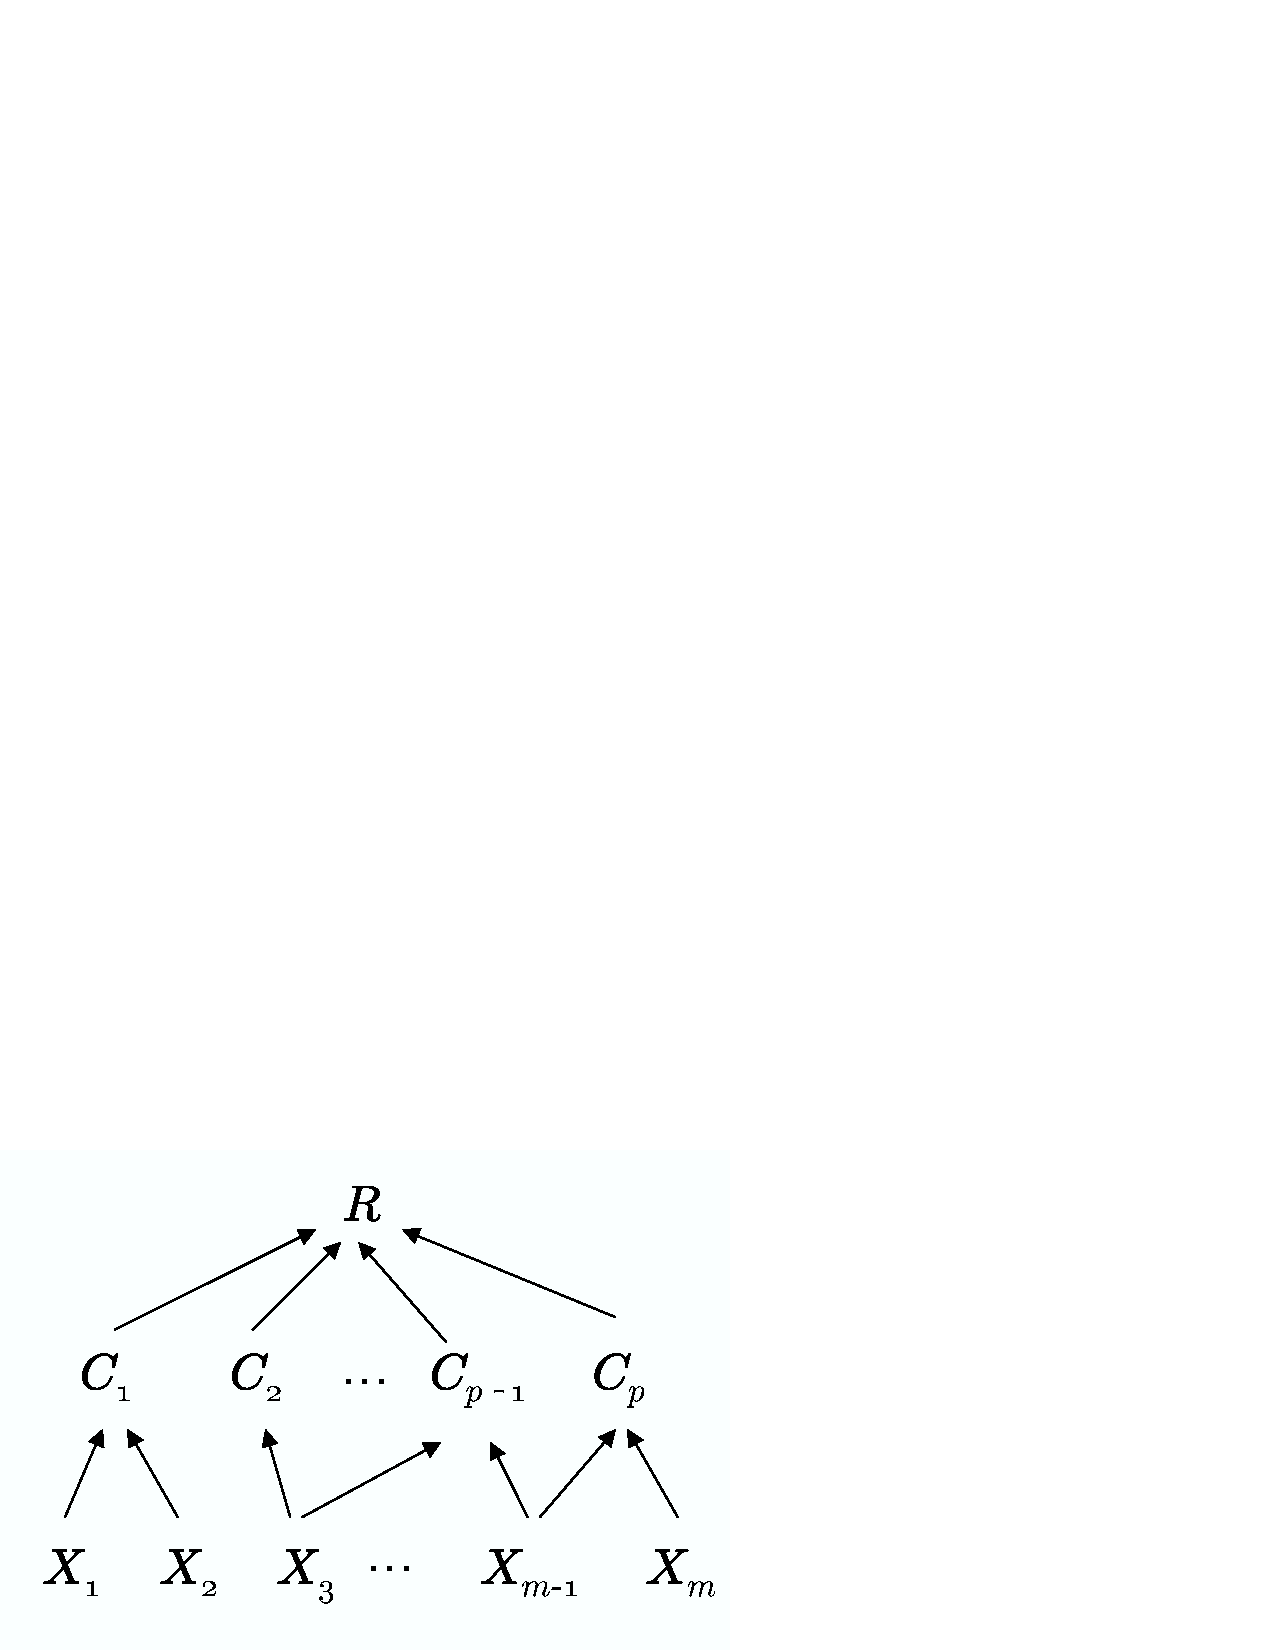
\includegraphics{pictures/target}
%%   % 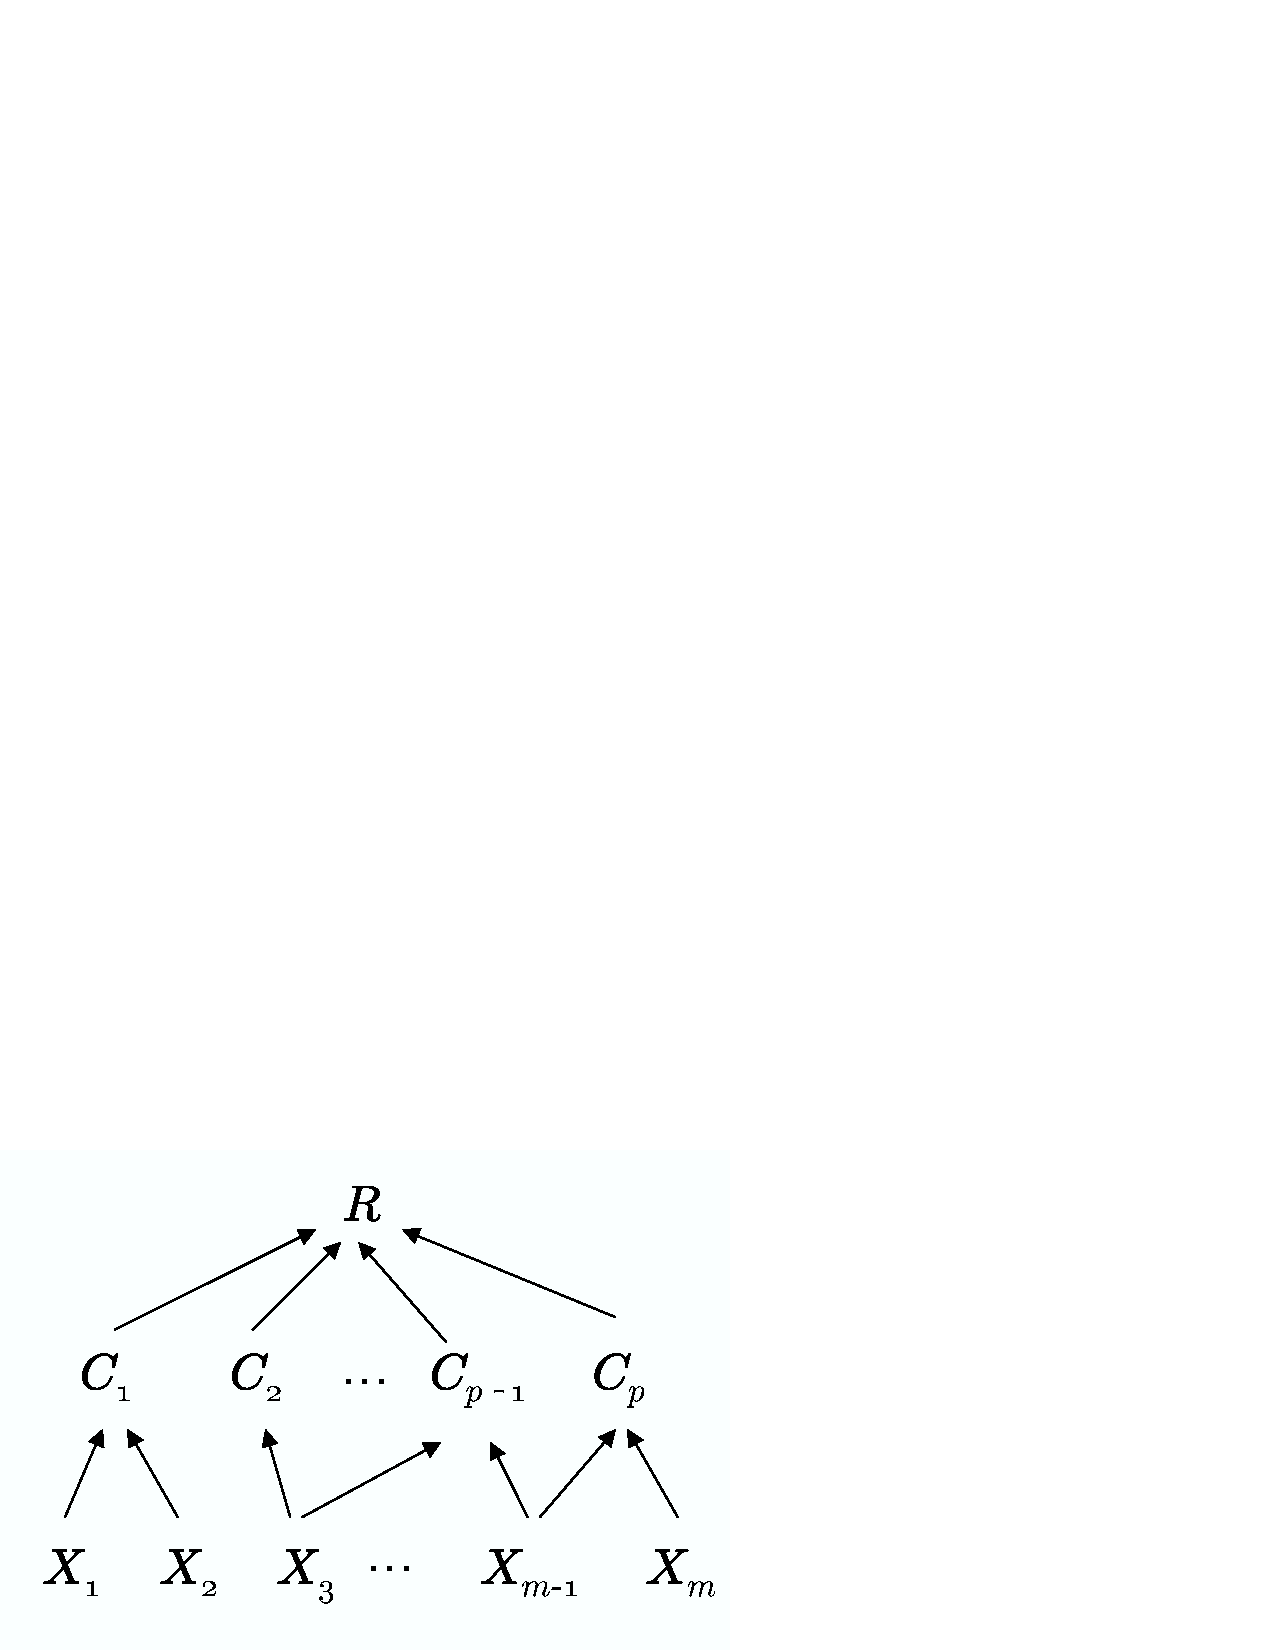
\includegraphics[width=1.8in]{pictures/target}
%%   \scalebox{0.3}{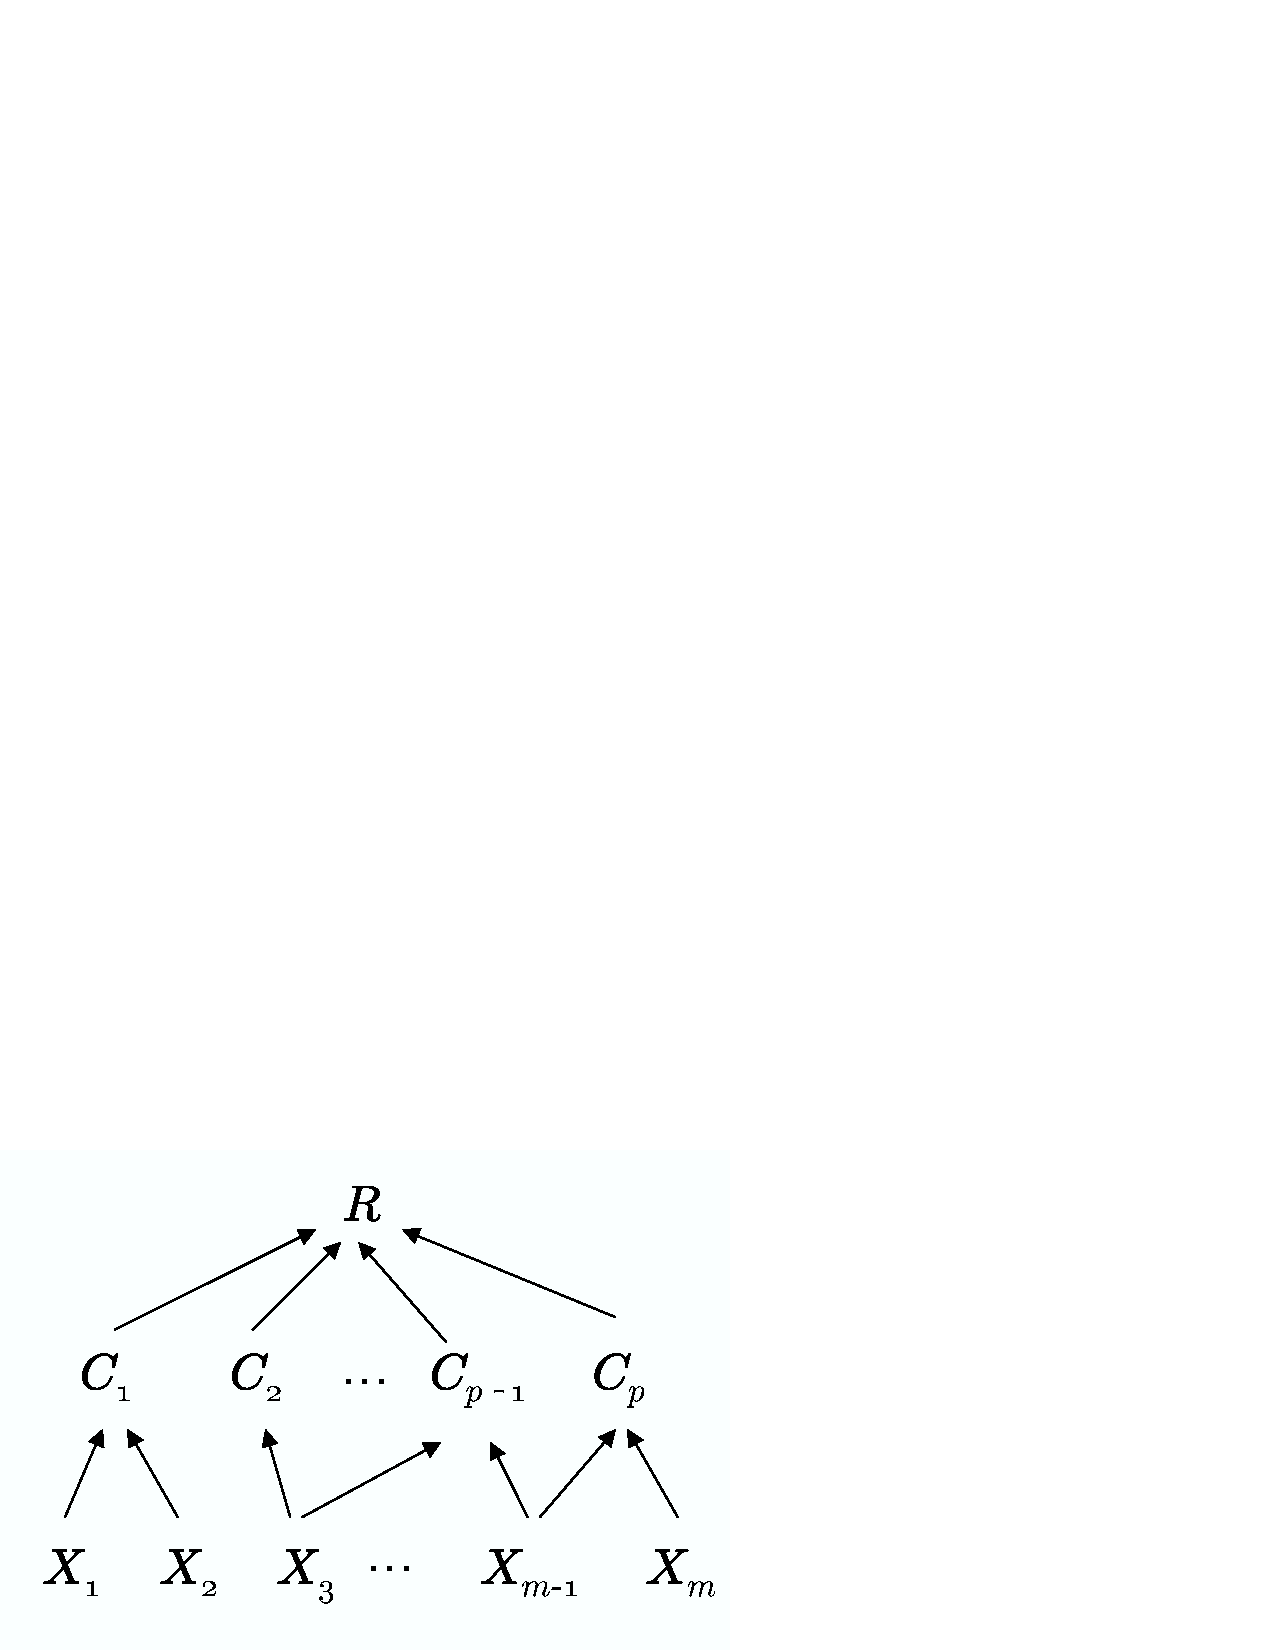
\includegraphics{pictures/target}}
%%   \caption{The basic graph for the $\NP$-hardness proof.
%%     A set cover of size $m$ corresponds to $m$ edges of the form $C \rightarrow R$.\newline}
%%   \label{fig:basic}
%%\end{figure}
%We show
%that if there is a unique I-map $G$ for $O$ with at most $k$ edges, then $G$ is a subgraph
%of the basic graph, with possibly edges $C_{i}\rightarrow R$
%missing for some sets $c_{i}$, such that the set of variables $\{C_{1},C_{2},\ldots,C_m\}$ with the edge $C%
%_{i}\rightarrow R$ in $G$ corresponds to an exact cover $\{c_{1},\ldots,c_{m}%
%\}$. Conversely, any unique exact cover corresponds to a subgraph of the basic
%graph in the same manner. %For reasons of space, we just illustrate most of the following assertions rather than giving full proofs.
%It is easiest to consider separately the constraints
%imposed by each clause of $O$. Let $\D_i$ be the {\em set of dependencies corresponding to Clause $i$.} For example, $D_{\ref{set}} = \{\langle C_i, X_j, \S \rangle: x_j \in c_i\}$. 
%%For example, $D_{\ref{emptyset}} = \{\langle X_j \dep R|\emptyset \rangle: j = 1,\ldots,3m\}$. 
%The implications of $\D_{\ref{set}}$ are as follows.

%% \emph{(1) Let graph }$G$\emph{\ be an I-map for }$\D_{\ref{set}}$\emph{. Then any two
%% variables }$X$\emph{\ and }$C$\emph{\ are adjacent whenever
%% }$ x \in c$\emph{.}
%\begin{assertion} \label{ass:adjacency}
%Let DAG $G$ be an I-map for $\D_{\ref{set}}$. Then any two
%%variables 
%nodes $X$ and $C$ are adjacent whenever
%$ x \in c$.
%\end{assertion}
%\begin{proof} The d-separation lemma \ref{lemma:d-sep} implies that if
%$G$ entails the dependencies in $\D_{\ref{set}}$, then $x$ and $C$ are adjacent
%whenever $x \in c$. \end{proof}
%%Next, let $\D_{member}$ be the
%%set of dependencies corresponding to Clause \ref{member}. 

%An implication of the constraints in
%$\D_{\ref{member}}$ is that any two element nodes $X_{i}, X_{j}$
%with $x_{i}, x_{j}$ contained in the same set $c$ are adjacent to each
%other or have variable $C$ as a common child (possibly both may be the case).

%\begin{assertion}
%Let DAG $G$ be an I-map for $\D_{\ref{set}}\cup \D_{\ref{member}}$, and suppose that $x_{i},x_{j}$ are two elements of a set $c$. Then $X_{i}$ and $X_{j}$ are adjacent in $G$, or $G$ contains a component $X_{i}\rightarrow C \leftarrow X_j$. \label{ass:set-adjacency}
%\end{assertion}
%\begin{proof} By Assertion \ref{ass:adjacency}, nodes $\X_{i}$ and $\X_{j}$ are respectively adjacent to $\C$. If $\X_{i}$ and $\X_{j}$ are adjacent, then the assertion holds trivially. 
%%Otherwise $\X_{i} - \C - \X_{j}$ forms an unshielded triple. \marginpar{is unshielded defined?} 
%A basic fact about d-separation is that in a triple $\X-\Y-\Z$ such that $\X$ and $\Z$ are not adjacent, the node $\Y$ is a collider if and only if all sets that contain $\Y$ d-connect $\X$ and $\Z$ \cite[Lemma 2.5]{neapolitan04:_learn_bayes_networ}. So the dependencies $\D_{\ref{member}}$ require that $\C$ is a collider in $G$.
%\end{proof}
%%Suppose for contradiction that $X_{i}$ and $X_{j}$ are not adjacent nor
%%are there two edges $X_{i}\rightarrow C$ and $X_{j}\rightarrow C$. Now by
%%Assertion (1), we have $X_{i}$ and $X_{j}$ adjacent to $C$. So there are two cases.

%%Case 1: DAG $G$ has the structure $C\rightarrow X_{i}$ and $X_{j}\rightarrow
%%C$. Let $Par(X_{i})$ be the set of parents in $G$; notice that $C\in
%%Par(X_{i})$. So the dependencies in $D_{members}$ require that $X_{i}$ and
%%$X_{j}$ be d-connected given $Par(X_{i})$. Now it is a basic fact about
%%d-separation that conditional on the parents $Par$ of a node $\v$,
%%another node $\mathbf{v}'$ is d-connected to $\v$ iff
%%$\mathbf{v}'$ is an ancestor of $\v$ [cite]. Therefore $X_{i}
%%$ is an ancestor of $X_{j}$ in $G$. But then $G$ contains a directed cycle
%%$X_{i}\rightarrow\cdots\rightarrow X_{j}\rightarrow C\rightarrow X_{i}$.

%%Case 2: DAG $G$ has the structure $C\rightarrow X_{i}$ and $C\rightarrow
%%X_{j}$. Let $C\in Par(X_{i})$ and $C\in Par(X_{j})$, so $X_{i}$ is d-connected
%%to $X_{j}$ given $Par(X_{i})$ and $X_{j}$ is d-connected to $X_{i}$ given
%%$Par(X_{j})$. By the basic fact cited above, this means that $X_{i}$ and
%%$X_{j}$ are descendants of each other, which implies that $G$ is not acyclic,
%%contrary to hypothesis.

%%So in either case, there is a contradiction, which establishes that $X_{i}$
%%and $X_{j}$ are adjacent in $G$, or $G$ contains two edges $X_{i}\rightarrow
%%C$ and $X_{j}\rightarrow C$.\emph{\ }

%%Let $\D_{\ref{emptyset}}$ be the set of dependencies corresponding to Clause \ref{clause:empty}.

%Clause \ref{emptyset} requires that every member variable $X$ be d-connected to the root
%variable. The intuition behind our reduction is that the basic graph $B$ contains the most
%edge-efficient way to achieve the connection because with just one edge
%$C \rightarrow R$ the graph d-connects three member variables at once. Since there are many
%ways to achieve d-connection in a graph, proving the correctness of this
%intuition is the main difficulty of our proof. 

%The bulk of the proof shows that any I-map for $\D_{\ref{emptyset}}$ can be
%transformed into a subgraph of the basic graph 
%$B$ without increasing the number of edges. This requires a number of intermediate results. %As a general notation for describing paths, we use \ldots
%We begin by establishing that in an I-map $G$ of $\D_{\ref{emptyset}}$, all arcs originating in the root variable $R$ can be reversed with the result $G'$ still an I-map of $\D_{\ref{emptyset}}$.
%%any edge $A\rightarrow V$ in an I-map of $\D_{\ref{emptyset}}$ can be reversed if $V$ is an ancestor of $R$ (making $V$ an ancestor of $R$),
%%with the result still entailing $\D_{\ref{emptyset}}$.

%%Proof: Suppose for contradiction that $X_{i}$ and $X_{j}$ are not adjacent nor
%%are there two edges $X_{i}\rightarrow C$ and $X_{j}\rightarrow C$. Now by
%%Assertion (1), we have $X_{i}$ and $X_{j}$ adjacent to $C$. So there are two cases.

%%Case 1: DAG $G$ has the structure $C\rightarrow X_{i}$ and $X_{j}\rightarrow
%%C$. Let $\Par(X_{i})$ be the set of parents of $X_i$ in $G$; notice that $C\in
%%\Par(X_{i})$. So the dependencies in $\D_{\ref{member}}$ require that $X_{i}$ and
%%$X_{j}$ be d-connected given $\Par(X_{i})$. Now it is a basic fact about
%%d-separation that conditional on the parents $Par$ of a node $V$,
%%another node $V'$ is d-connected to $V$ iff
%%$V'$ is an ancestor of $V$ \cite[Cor.3.4]{pearl88:_probab_reason_intel_system}. Therefore $X_{i}
%%$ is an ancestor of $X_{j}$ in $G$. But then $G$ contains a directed cycle
%%$X_{i}\rightarrow\cdots\rightarrow X_{j}\rightarrow C\rightarrow X_{i}$.

%%Case 2: DAG $G$ has the structure $C\rightarrow X_{i}$ and $C\rightarrow
%%X_{j}$. Let $C\in \Par(X_{i})$ and $C\in \Par(X_{j})$, so $X_{i}$ is d-connected
%%to $X_{j}$ given $\Par(X_{i})$ and $X_{j}$ is d-connected to $X_{i}$ given
%%$\Par(X_{j})$. By the basic fact cited above, this means that $X_{i}$ and
%%$X_{j}$ are descendants of each other, which implies that $G$ is not acyclic,
%%contrary to hypothesis.

%%%So in either case, there is a contradiction, which establishes that $X_{i}$
%%%and $X_{j}$ are adjacent in $G$, or $G$ contains two edges $X_{i}\rightarrow
%%%C$ and $X_{j}\rightarrow C$.\emph{\ }

%%Since there are many
%%ways to achieve d-connection in a graph, proving the correctness of this
%%intuition is the main difficulty of our proof. We begin by considering the
%%simple case of Clause 1 in which we don't condition on any variables. This
%%corresponds to the clause "If $V_{1}=R,V_{2}=X%
%%_{j},W\mathbf{=\emptyset},$ then return 'dependent'.\newline" Let
%%$\D_{\ref{emptyset}}$ be the dependencies defined by this clause. The reason why
%%$\D_{\ref{emptyset}}$ is easier to analyze than the complete set of dependencies
%%$\D_{cover}$ is that d-separation is simpler without conditioning variables.
%%Obviously any I-map for $\D_{cover}$ is also an I-map for $\D_{\ref{emptyset}}$.
%%Moreover, we will show that there is an I-map that is minimal for both
%%$\D_{\ref{emptyset}}$ and $\D_{cover}$ (namely a subgraph of the basic graph). This
%%means that any minimum I-map for $\D_{cover}$ must also be a minimal I-map for
%%$\D_{\ref{emptyset}}$. Thus necessary conditions for minimal I-maps for
%%$\D_{\ref{emptyset}}$ holds also for $\D_{cover}$.
%%

%\begin{lemma} \label{ass:reverse-root}
%Let DAG $G$ be an I-map of $\D_{\ref{emptyset}}$. Let
%$G'$ be the graph obtained by reversing all arcs of the form
%$R\rightarrow V$ to be $V\rightarrow R$. 
%Then $G'$ is an I-map of $\D_{\ref{emptyset}}$.
%\end{lemma}
%%Illustration of the basic idea: Suppose $G$ contains a component $R \rightarrow X \rightarrow X'$. Reverse the edge $R \rightarrow X$ to obtain $G'$. Consider the d-connecting path $R \rightarrow X \rightarrow X'$ in $G$. 
%%In any such path in $G'$ 
%%we can replace the edge $R \rightarrow X$ by $R \leftarrow X$  in $G'$ without introducing additional colliders, so d-connection still holds.

%\begin{proof}First we argue that $G'$ is acyclic. Suppose for contradiction
%that $G'$ contains a directed cycle %$\X \rightarrow\cdots\rightarrow \X$
%that is not contained in $G$. Then the cycle involves a reversed edge of the
%form $\X \rightarrow R$, and we can write the cycle as $\R \rightarrow
%\Y \rightarrow \cdots\rightarrow \R$. However, since all
%edges involving the root $\R$ are reversed in $G'$, there is no edge
%$\R \rightarrow \Y$ in $G'$. So $G'$ is acyclic since $G$
%is.

%Second, we show that $G'$ entails the dependencies in $\D_{\ref{emptyset}}$.
%Let $X$ be any member variable and consider a path $p$ in $G$ of the form
%$$p=R-\cdots-X$$ that d-connects $R$ and $X$ in $G$. 
%%Let $\ZZ$ be the set of
%%variables that had an edge reversed, i.e., $\X\in Z\iff R\rightarrow \X$ is an
%%edge in $G$.

%Case 1: The path $p$ contains no reversed edge. %member of $\ZZ$. 
%Then the edges in $p$ are the
%same in $G$ as in $G'$, and $p$ d-connects $R$ and $X$ in $G'$.

%Case 2: The path $p$ contains some reversed edge. Let $\Z$ be the last such
%member. Then $p$ is of the form $$p=\R-\cdots-\Z-\cdots-\X$$ where the final path
%segment $\Z-\cdots-\X$ contains no nodes with their edges changed. The following
%path $p'$ d-connects $\R$ and $\X$ in $G'$: set $$p^{\prime
%}=\R\leftarrow \Z-\cdots-\X.$$ Clearly the node $\Z$ is not a collider in
%$p'$, and so $p'$ d-connects $\R$ and $\X$ in $G' $ as
%the final segment $\Z-\cdots-\X$ is oriented the same in both graphs.
%So in either case, $\R$ and $\X$ are d-connected in $G'$ and so
%$G'$ entails $\D_{\ref{emptyset}}$.
%\end{proof}

%%The proof of the following two assertions employs the same basic argument.
%The next assertion shows that if the root node is a sink in a graph $\G$, then for any parent $\A$ of $\R$, all edges pointing out of $\A$ except for $\A \rightarrow \R$ can be reversed.
%%\begin{assertion} \label{ass:reverse}
%%{Let DAG }$G${\ be an I-map of }$\D_{\ref{emptyset}}$. Suppose that where $\A$ is an ancestor of the root variable $\R$. Let $G'$ be the
%%graph obtained by reversing all edges of the form $\A \rightarrow \B$, where 
%%$\A$ is an ancestor of the root variable $\R$ (including a nonproper ancestor where $\A = \R$) and 
%%$\B$ is not an ancestor of $R$. %to
%%%be $\A \leftarrow \B$. 
%%Then $G'$ is an I-map of $\D_{\ref{emptyset}}$.
%% \end{assertion}
%%Illustration: Suppose $G$ contains a component $X \leftarrow X' \rightarrow C \rightarrow R$. Reverse the edge $X \leftarrow X'$ to obtain $G'$. Consider the d-connecting path $X \leftarrow X' \rightarrow C \rightarrow R$ in $G$. In any such directed path in $G'$ we can replace the edge $X \leftarrow \X'$ by $X \rightarrow X'$  in $G'$ without introducing additional colliders, so d-connection still holds. 

%\begin{lemma} \label{ass:reverse}
%{Let DAG }$G${\ be an I-map of }$\D_{\ref{emptyset}}$. Suppose that the root variable $\R$ has outdegree 0 and that $\A$ is a parent of $\R$ in $\G$. Let $G'$ be the
%graph obtained by reversing all edges of the form $\A \rightarrow \B$ where $\B \neq \R$. Then $G'$ is an I-map of $\D_{\ref{emptyset}}$.
% \end{lemma}
%%[Illustration: Suppose $G$ contains a component $X \leftarrow X' \rightarrow C \rightarrow R$. Reverse the edge $X \leftarrow X'$ to obtain $G'$. Consider the d-connecting path $X \leftarrow X' \rightarrow C \rightarrow R$ in $G$. In any such directed path in $G'$ we can replace the edge $X \leftarrow \X'$ by $X \rightarrow X'$  in $G'$ without introducing additional colliders, so d-connection still holds. ]

%\begin{proof} 
%First we argue that $G'$ is acyclic. 
%%[Basically, cycle involves an edge with C. But then the cycle points into R, which is a sink. ] 
%Suppose for contradiction
%that $G'$ contains a directed cycle 
%that is not contained in $G$. Then the cycle involves a reversed edge and hence contains $\A$, so without loss of generality, we may assume the cycle is of the form $\A \rightarrow \cdots \rightarrow \A$. But the only child of $\A$ in $\G'$ is the root $\R$, which is a sink in $\G$ and hence in $\G'$. So there is no directed path from $\R$ to $\A$ and hence no directed cycle in $\G'$ from $\A$ to $\A$. Thus $G'$ is acyclic since $G$ is.
%%\Y \rightarrow \cdots\rightarrow \R$. However, since all
%%edges involving the root $\R$ are reversed in $G'$, there is no edge
%%$\R \rightarrow \Y$ in $G'$. So $G'$ is acyclic since $G$
%%is.
%%We note that $G'$ is acyclic by the same argument as in
%%Assertion \ref{ass:reverse-root}. 

%To see that $G'$ entails the dependencies in
%$D_{\ref{emptyset}}$, let $X$ be any member variable; since $\G$ entails the dependencies in $\D_{\ref{emptyset}}$, there is a path $p$ in $G
%$ of the form $R-\cdots-X$ that d-connects $R$ and $X$ in $G$. 
%%Let $Z$ be the
%%set of variables that had an edge reversed, i.e., $V\in Z\iff a\rightarrow v$
%%is an edge in $G$.
%%
%%Case 1: If path $p$ uses an edge of the form $\Av$, it is oriented as
%%$V\rightarrow a$. Then the edges in $p$ are the same in $G$ as in $G'
%%$, and $p$ d-connects $R$ and $X$ in $G'$.
%Suppose that path $\p$ uses an edge of the form $\A \rightarrow \B$ that is reversed in $G'$.

%Case 1: $p$ is of the form $$\X - \cdots - \A \rightarrow \B \rightarrow \cdots \rightarrow \R.$$ Then the path $$\X - \cdots - \A \rightarrow \R$$ d-connects $\X$ and $\R$ in $\G'$.

%Case 2: $p$ is of the form $$\X - \cdots \leftarrow \B \leftarrow \A - \cdots - \R.$$ Then the path $$\X - \cdots \leftarrow \B \leftarrow \A \rightarrow \R$$ introduces no new collider and thus d-connects $\X$ and $\R$ in $\G'$. So all member variables $\X$ are d-connected to the root variable $\R$ in $\G'$ and $\G'$ is an I-map of the dependencies $D_{\ref{emptyset}}$. 
%\end{proof}

%The next assertion shows that if a node has two directed paths towards the root, then one of them is superfluous for entailing the dependencies in $\D_{\ref{emptyset}}$, and it is possible to delete an edge. This is a key fact for constraining the structure of edge-minimal graphs.

%\begin{lemma} \label{ass:delete}
%Let DAG $G$ be an I-map of $\D_{\ref{emptyset}}$. Suppose
%that for some node $\X$, there are two directed paths $\X \rightarrow
%U_{1}\rightarrow\cdots\rightarrow U_{p}\rightarrow R$ and
%$\X \rightarrow W_{1}\rightarrow\cdots\rightarrow W_{q}\rightarrow R$ where $\U_{1} \neq \W_{1}$.
%Let $G'$\ be the graph obtained from $G$\ by deleting
%the edge $\X \rightarrow U_{1}$. Then $G'$\ is an I-map of
%$\D_{\ref{emptyset}}$.
%\end{lemma}

%%Illustration: Suppose $G$ contains two paths $\X \rightarrow C \rightarrow R$ and $\X \rightarrow X' \rightarrow R$. Delete the edge $\X \rightarrow X'$ to obtain $G'$. Then $\X$ remains d-connected to $R$. A d-connecting path to $R$ in $G$ using the edge $\X \rightarrow X'$ can be ``rerouted'' via either $\Y$ or $X'$.

%\begin{proof}
%%%Similar to claims \ref{ass:reverse-root} and \ref{ass:reverse} above. 
%%Let $X$ be any %member 
%%variable and
%Consider a path $p$ in $G$ of the form $$p=\R-\cdots-\Y$$ that d-connects $R$ and
%$\Y$ in $G$. If $p$ does not use the edge $\X \rightarrow U_{1}$, then $\p$
%d-connects $\R$ and $\X$ in $G'$. Otherwise there are two cases.

%Case 1: The path $\p$ is of the form $$p=R-\cdots-\X \rightarrow \U_{1}-\cdots-\Y.$$ Then $\Y$ is d-connected to $\U_{1}$ in $\G$ and hence in $\G'$. Thus the path $$\Y-\cdots-\U_{1} \rightarrow\cdots\rightarrow U_{p}\rightarrow \R$$ d-connects $\Y$ to $\R$.

%Case 2: The path $\p$ is of the form $$p=R-\cdots-\U_{1} \leftarrow \X-\cdots-\Y.$$ Since $\U_{1} \neq \W_{1}$, the path $$\X \rightarrow W_{1}\rightarrow\cdots\rightarrow W_{q}\rightarrow R$$ exists in $\G'$. So the path $$\Y-\cdots-\X  \rightarrow W_{1}\rightarrow\cdots\rightarrow W_{q}\rightarrow \R$$ d-connects $\Y$ to $\R$.

%So in either case, any member variable $\Y$ is d-connected to the root variable $\R$ in the graph $\G'$, and so $\G'$ is an I-map of $\D_{\ref{emptyset}}$.
%\end{proof}

%\begin{lemma} \label{lemma:delete2}
%Let DAG $\G$ be an I-map of $\D_{\ref{emptyset}}$. Suppose $\G$ contains an edge $\A \rightarrow \B$ where $\B$ is not an ancestor of $\R$. Add an edge $\B \rightarrow \R$ and delete the edge $\A \rightarrow \B$. The resulting graph $\G'$ is an I-map of $\D_{\ref{emptyset}}$ that contains no more edges than $\G$.
%\end{lemma}

%\begin{proof}
%Consider any path in $\G$ that d-connects a member variable $\X$ with root variable $\R$ and uses the edge $\A \rightarrow \B$. Since $\B$ is not an ancestor of $\R$, the path must be of the form $$\X - \cdots \leftarrow \B \leftarrow \A - \cdots - \R.$$ So in $\G$ there is a path $\X -\cdots  \leftarrow \B$ that does not involve the edge $\A \rightarrow \B$, hence in $\G'$ we have the path $$\X -\cdots  \leftarrow \B \rightarrow \R$$ d-connecting $\X$ and $\R$. So any member variable d-connected to $R$ in $G$ is also d-connected in $\G'$, which establishes the lemma.
%\end{proof}
%%
%%that for some node $\X$, there are two directed paths $\X \rightarrow
%%U_{1}\rightarrow\cdots\rightarrow U_{p}\rightarrow R$ and
%%$\X \rightarrow W_{1}\rightarrow\cdots\rightarrow W_{q}\rightarrow R$ where $\U_{1} \neq \W_{1}$.
%%Let $G'$\ be the graph obtained from $G$\ by deleting
%%the edge $\X \rightarrow U_{1}$. Then $G'$\ is an I-map of
%%$\D_{\ref{emptyset}}$.
%%\end{assertion}

%The previous lemmas showed that an I-map $\G$ of $\D_{\ref{emptyset}}$ can be transformed in various ways that bring it closer to the basic graph while still remaining an I-map. The next key Assertion \ref{ass:lower-bound} shows that an I-map $\G$ of $\D_{\ref{emptyset}}$ of minimum size must not contain certain types of edges outside of the basic graph; we refer to these as `inefficient' edges. Formally, say that an edge is {\em inefficient} in DAG $\G$ if and only if it has one of the following forms: (1) $\X - \Y$ where $\X$ and $\Y$ are member variables, (2) $\X - \R$ where $\X$ is a member variable, (3) $\X \rightarrow \C$ where $\x \not\in \c$. An edge is efficient if it is not inefficient. So the efficient edges have one of the following forms: (1) $\C - \R$, or (2) $\C - \C'$, or (3) $\C - \X$ with $\x \in \c$, or (4) $\X \leftarrow \C$ where $\x \not\in \c$; here $\C,\C'$ are set variables, and $\X$ is a member variable. We refer to an adjacency of the form $\X \leftarrow \C$ where $\x \not\in \c$ as an {\em efficient set-nonmember link.} We show that the presence of an inefficient edge in an I-map of $\D_{\ref{set}}\cup \D_{\ref{member}}\cup
%\D_{\ref{emptyset}}$ requires more than $k$ edges total in $\G$, by the following construction: First, if an I-map of $\D_{\ref{set}}\cup \D_{\ref{member}}\cup
%\D_{\ref{emptyset}}$ contains no efficient set-nonmember links, but contains inefficient edges, then it has more than $k$ edges total. Second,
%we can replace efficient set-nonmember links with other links, without reducing the number of inefficient edges, until the first case applies.
%%  The next lemma shows that in an I-map of $\D_{\ref{set}}\cup \D_{\ref{member}}\cup
%%\D_{\ref{emptyset}}$ we can replace an inefficient set-nonmember link by another type of inefficient link while still entailing all the required dependencies. Thus we can reduce graphs with inefficient links to those containing inefficient links that are not set-nonmember links.
% 
%% \begin{lemma} \label{lemma:abnormal}
%%Let $\G$ be an I-map of $\D_{\ref{set}}\cup \D_{\ref{member}}\cup
%%\D_{\ref{emptyset}}$. There is a graph $\G'$ such that (1)
%%$\G'$ is an I-map of $\D_{\ref{set}}\cup \D_{\ref{member}}\cup
%%\D_{\ref{emptyset}}$, (2) $\G'$ contains no more edges than $\G$, (3) $\G'$ contains one less set-nonmember link, and (4) $\G'$ contains all inefficient edges contained in $\G$ that are not set-nonmember links.
%%\end{lemma}
%% 
%% \begin{proof}
%%Consider an inefficient set-nonmember link $\X \rightarrow \C$ with $\x \not\in \c$.  By Assertions \ref{ass:adjacency} and \ref{ass:set-adjacency} we may delete the link $\X \rightarrow \C$ with the result still an I-map of $\D_{\ref{set}}\cup \D_{\ref{member}}$. 
%%%Let the link be oriented as $\A \rightarrow \B$.

%%%Let $\x$ be contained in some set $c'$. 
%%%
%% 
%%Case 1a: The variable $\C$ is is not an ancestor of $\R$. Then add an edge $\X \rightarrow \R$ and delete the edge $\X \rightarrow \C$. By Lemma \ref{lemma:delete2}, the resulting graph $\G'$ is an I-map of $\D_{\ref{set}}\cup \D_{\ref{member}}\cup
%%\D_{\ref{emptyset}}$.

%%Case 1b: The variable $\C$ is  an ancestor of $\R$. Add an edge $\X \rightarrow \R$. Then there are two directed paths from $\X$ to $\R$, namely $\X \rightarrow \R$ and $\X \rightarrow \C \rightarrow \cdots \R$, so by Lemma \ref{ass:delete}, we may delete the edge $\X \rightarrow \R$ with the result being an I-map of $\D_{\ref{set}}\cup \D_{\ref{member}}\cup
%%\D_{\ref{emptyset}}$. 

%%Thus in all cases, we can reduce the number of inefficient set-nonmember links by 1 meeting the conditions of the Lemma. 
%%\end{proof}

%

% \begin{assertion} \label{ass:lower-bound}
%Let $\G$ be an I-map of $\D_{\ref{set}}\cup \D_{\ref{member}}\cup
%\D_{\ref{emptyset}}$. If $\G$ contains inefficient edges, then $\G$ contains more than $k = 3p+m$ edges. 
%\end{assertion}

%\begin{proof}
%The proof is by induction on the number of efficient set-nonmember links, denoted as $a$.

%Base Case, $a = 0$. We proceed with a further induction on  the number of inefficient edges, denoted as $i$.
%Base Case, $i = 1$. 
%Let $\A \rightarrow \B$ be the only inefficient edge in $\G$, and suppose for contradiction that $\G$ contains no more than $3p + m$ edges. Assertion \ref{ass:adjacency}  implies that $\G$ contains $3p$ adjacencies of the form $\X - \C$ where $\x \in \c$, which are efficient. Since $\G$ contains also an inefficient edge, the number of remaining efficient edges not of the form $\X - \C$ is at most $$(3p + m) - 3p -1 = m-1.$$
%Let $\C$ be any set variable; as $\c$ contains three elements, and there is only one inefficient edge in $\G$, there is an element $\x \in \c$ such that $\X$ is not adjacent to any other member variable $\X'$ with $\x'$ in $\c$. So by Assertion \ref{ass:set-adjacency}, all $3p$ adjacencies $\X - \C$ with $\x \in \c$ are oriented as $\X \rightarrow \C$. So no edge of the form $\C \rightarrow \A$ is included in the $3p$ links $\X \rightarrow \C$, and since all edges of the form $\C \rightarrow \A$ are efficient by definition, it follows that there are at most $m-1$ such edges. In other words, there are at most $m-1$ set variables that have outdegree greater than 0. So there are at most $3(m-1) = 3m-3$ elements $\x$ of the universe such that $\X$ is adjacent to some set variable $\C$ with outdegree greater than 0. The contrapositive of this conclusion is that at least three elements $x,y,z$ are adjacent only to set variables with outdegree 0. At least one of the corresponding nodes $\X,\Y,\Z$ is distinct from $\A$ and $\B$; without loss of generality, choose $\X$ to be the distinct one. As all edges linking $\X$ are efficient, edges linking $\X$ are of the form $\X \rightarrow \C$ with $\x \in \c$ and $\X \leftarrow \C$ where $\x \not\in \c$. But since $\X$ is adjacent only to set variables with outdegree 0, the latter type of edge does not exist, and so all edges linking $\X$ are of the form $\X \rightarrow \C$ where $\x \in \c$ and the set variable $\C$ has outdegree 0. Any path that d-connects $\X$ and $\R$ has to start with an edge $\X \rightarrow \C \rightarrow \cdots - \R$; since there is no such path, the graph $\G$ fails to entail the dependencies $\D_{\ref{emptyset}}$. This contradiction shows that $\G$ has more than $3p+m$ edges.

%Inductive Step (still with $a = 0$): Assume the hypothesis for $i$ and consider $i+1$. 

%We show how to transform $\G$ into an I-map $\G'$ of $\D_{\ref{set}}\cup \D_{\ref{member}}\cup
%\D_{\ref{emptyset}}$ with one less inefficient edge and no more edges overall. The inductive hypothesis then implies that $\G'$ and hence $\G$ has more than $k$ edges. 

%\begin{enumerate}
%\item Reorient all edges to point into the root $\R$. By Lemma \ref{ass:reverse-root}, the result $\G_1$ is an I-map of $\D_{\ref{set}}\cup \D_{\ref{member}}\cup
%\D_{\ref{emptyset}}$ with the same number of edges; the number of inefficient edges is the same.
%\item If $\G_1$ contains an edge $\X \rightarrow \R$, where $\X$ is a member variable, then: 
%\label{step:member-root}
%\begin{enumerate}
%\item Choose a set variable $\C$ with $\x \in \c$, and add an edge $\C \rightarrow \R$ (such an edge may already exist in $\G_1$). \label{step:addedge}
%\item Reorient any adjacency $\B \leftarrow \C$ to point into $\C$, where $\B \neq \R$. By Lemma \ref{ass:reverse}, the result $\G_2$ is  an I-map of $\D_{\ref{emptyset}}$. And by Assertions \ref{ass:adjacency} and \ref{ass:set-adjacency} $\G'$ is also an I-map of $\D_{\ref{set}}\cup \D_{\ref{member}}$. Since there are no efficient set-nonmember links ($a=0$), it is not possible to have $\B = \X$ with $\x \not\in \c$, so this step adds no inefficient edges. \label{steporient}

%\item Delete the edge $\X \rightarrow \R$. Since in $\G_2$ there are two directed paths connecting $\X$ to $\R$, namely $\X \rightarrow  \R$ and $\X \rightarrow \C \rightarrow \R$, Lemma \ref{ass:delete} guarantees that the resulting graph is an I-map of $\D_{\ref{set}}\cup \D_{\ref{member}}\cup
%\D_{\ref{emptyset}}$. As the construction adds an edge in step \ref{step:addedge} and deletes one in this step, the overall number of edges is the same as in $\G$. Since no inefficient edge was added and this step deletes an inefficient edge, the number of inefficient edges has decreased by 1 as required. 
%\end{enumerate}
%\item Else if $\G_1$ contains an adjacency $\X - \Y$ where $\X$ and $\Y$ are member variables, suppose without loss of generality that the link is oriented as $\X \rightarrow \Y$. \label{step:members}
%\begin{enumerate}
%\item If $\Y$ is an ancestor of the root $\R$, then:

%\begin{enumerate}
%\item Choose a set variable $\C$ with $\x \in \c$, and add an edge $\C \rightarrow \R$ (such an edge may already exist in $\G_1$).

% 
%\item Reorient any adjacency $\B \leftarrow \C$ to point into $\C$, where $\B \neq \R$. As in Steps \ref{step:addedge} and \ref{steporient} above, the result $\G_2$ is an I-map of $\D_{\ref{set}}\cup \D_{\ref{member}}\cup
%\D_{\ref{emptyset}}$ with no added inefficient edges and at most one more edge overall.
%\item Delete the edge $\X \rightarrow \Y$. Since in $\G_2$ there are two directed paths connecting $\X$ to $\R$, namely $\X \rightarrow  \Y \rightarrow \cdots \rightarrow \R$ and $\X \rightarrow \C \rightarrow \R$, Lemma \ref{ass:delete} guarantees that the resulting graph is an I-map of $\D_{\ref{set}}\cup \D_{\ref{member}}\cup
%\D_{\ref{emptyset}}$. As the construction adds an edge in step \ref{step:addedge} and deletes one in this step, the overall number of edges is the same as in $\G$. Since no inefficient edge was added and this step deletes an inefficient edge, the number of inefficient edges has decreased by 1 as required.
%\end{enumerate}
%\item Else if $\Y$ is not an ancestor of the root $\R$, add an edge $\Y \rightarrow \R$ and delete the edge $\X \rightarrow \Y$. Lemma \ref{lemma:delete2} implies that the result is an I-map of $\D_{\ref{set}}\cup \D_{\ref{member}}\cup
%\D_{\ref{emptyset}}$. Then proceed as in Step \ref{step:member-root} to eliminate the edge $\Y \rightarrow \R$.
%In the resulting graph, the number of edges is the same as in the original graph $\G$ and there is one less inefficient edge, as required.
%\end{enumerate}
%\item Else if $\G_{1}$ contains an adjacency $\X \rightarrow \C$ where $\x \not\in \c$, proceed as in Step \ref{step:members} with $\C$ in place of $\Y$.
%\end{enumerate}

%
%This construction covers all cases of inefficient edges and completes the base case, $a=0$, in which there no efficient set-nonmember links.

%Inductive Step: Assume the hypothesis for $a$ and consider $a+1$. Let $\X \leftarrow \C$ be an efficient set-nonmember link in $\G$ such that $\x \not\in \c$. We show how to transform $\G$ into an I-map $\G'$ of $\D_{\ref{set}}\cup \D_{\ref{member}}\cup
%\D_{\ref{emptyset}}$, where $\G'$ has one less efficient set-nonmember link edge, at least as many inefficient edges as  $\G$ and no more edges than $\G$ overall. The inductive hypothesis for $a$ then implies that $\G'$ and hence $\G$ has more than $k$ edges.  
%\begin{enumerate}
%\item If the variable $\X$ is is not an ancestor of $\R$, then add an edge $\X \rightarrow \R$ and delete the edge $\X \leftarrow \C$. By Lemma \ref{lemma:delete2}, the resulting graph $\G'$ is an I-map  of $\D_{\ref{emptyset}}$. And by Assertions \ref{ass:adjacency} and \ref{ass:set-adjacency} $\G'$ is also an I-map of $\D_{\ref{set}}\cup \D_{\ref{member}}$. Since one inefficient edge was added and one efficient set-nonmember edge was deleted, the graph $\G'$ has the same number of edges overall and more inefficient edges than $\G$.
%\item Else add an edge $\C \rightarrow \R$. Then there are two directed paths from $\C$ to $\R$, namely $\C \rightarrow \R$ and $\C \rightarrow \X \rightarrow \cdots \rightarrow \R$, so by Lemma \ref{ass:delete}, we may delete the edge $\C \rightarrow \X$ with the result being an I-map of $\D_{\ref{emptyset}}$. And by Assertions \ref{ass:adjacency} and \ref{ass:set-adjacency} $\G'$ is also an I-map of $\D_{\ref{set}}\cup \D_{\ref{member}}$. Since one efficient edge was added and one efficient set-nonmember edge was deleted, the graph $\G'$ has the same number of edges overall and as many inefficient edges as $\G$.
%\end{enumerate}
%This construction completes the inductive step; by inductive hypothesis, $\G'$ and thus $\G$ has more than $k$ edges. Thus any I-map $\G$ of $\D_{\ref{set}}\cup \D_{\ref{member}}\cup
%\D_{\ref{emptyset}}$ that contains an inefficient edge has more than $k$ adjacencies.
%\end{proof}
%%
%% 
%%Let $\G$ be a DAG. Say that an edge is inefficient in $\G$ if and only if it has one of the following forms: (1) $\X - \Y$ where $\X$ and $\Y$ are member variables, or (2) $\X - \R$ where $\X$ is a member variable, or (3) $\X \rightarrow \C$ where $\x \not\in \c$. An edge is efficient if it is not inefficient. So the efficient edges have one of the following forms: (1) $\C - \R$, or (2) $\C - \C'$, or (3) $\C - \X$ with $\x \in \c$, or (4) $\X \leftarrow \C$ where $\x \not\in \c$.

%The next Assertion shows that the number $k = 3p +m$ is a lower bound on the number of edges in an I-map of $\D_{\ref{set}}\cup \D_{\ref{member}}\cup
%\D_{\ref{emptyset}}$. Combined with the previous assertion, we obtain strong constraints on the structure  of a minimum-edge I-map of $\D_{\ref{set}}\cup \D_{\ref{member}}\cup
%\D_{\ref{emptyset}}$.

%\begin{assertion} \label{ass:unique-path}
%Let DAG $\G$ be an I-map of  $\D_{\ref{set}}\cup \D_{\ref{member}}\cup
%\D_{\ref{emptyset}}$ with no more than $k = 3p +m$ adjacencies. 
%\begin{enumerate}
%\item Every member variable $\X$ is an ancestor of the root variable $\R$. \label{clause:ancestor} 
%\item The DAG $\G$ contains exactly $k$ edges, and the collection $\{\c: \C \mbox{ has outdegree 1}\}$ is a partition of the universe. \label{clause:exact-bound}
%\item For every ancestor $\A$ of $\R$, there is exactly one d-connecting path to $\R$. \label{clause:unique-path} 
%\end{enumerate}

%\end{assertion}
% 
% \begin{proof}
%Part \ref{clause:ancestor}: Let $\X$ be any member variable. Suppose for contradiction that $\X$ is not an ancestor of $\R$. Then any d-connecting path from $\X$ to $\R$ must be of the form 
% $$\X \leftarrow \C-\cdots-\R$$ where $\x \not\in \c$, since by Assertion \ref{ass:lower-bound} $\G$ contains only efficient edges. Now by Lemma \ref{lemma:delete2} we may add an edge $\X \rightarrow \R$ and delete the edge $\X \leftarrow \C$ with the result $\G'$ still an I-map of $\D_{\ref{set}}\cup \D_{\ref{member}}\cup
%\D_{\ref{emptyset}}$. But then $\G'$ contains the inefficient edge $\X \rightarrow \R$, so by Assertion \ref{ass:lower-bound}, it has more than $k$ edges, so $\G$ has more than $k$ edges, which is a contradiction.

%Part \ref{clause:exact-bound}: Since $\G$ contains only efficient edges, Part \ref{clause:ancestor} implies that for every member variable $\X$, there is a set variable $\C$ with an edge $\X \rightarrow \C$ in $\G$ such that $\C$ is an ancestor of $\R$, and $\C$ has outdegree greater than 0. So the collection $\{\c: \C \mbox{ is an ancestor of $\R$}\}$ covers the universe $U$, and the size of this collection is at least $m$. On the other hand, for every member $\c$ of this collection, the corresponding set variable $\C$ has an edge originating in it, and overall there can be at most $m$ such edges: for the graph contains a total of no more than $m + 3p$ adjacencies and $3p$ of the adjacencies are of the form $\X \rightarrow \C'$ for $\x \in \c'$. So the size of the collection $\{\c: \C \mbox{ is an ancestor of $\R$}\}$  is exactly $m$, which establishes that $\G$ contains exactly $m + 3p = k$ edges. Also, the collection is a partition of the universe. Thus (a) every set variable $\C$ has outdegree at most 1, and indegree exactly 3, (b) $\C$ has outdegree 1 if and only if  $\C$ is an ancestor of $\R$, and (c) every member variable $\X$ points to exactly one set variable $\C$ with outdegree 1.

%Part \ref{clause:unique-path}: 
%First we argue that if $p$ is a path d-connecting an ancestor $\A$ to the root variable $\R$, then $p$ is directed. % andhas the form $\A \rightarrow \cdots \rightarrrow \R$. 
%The proof is by induction on the length $l >0$ of the path $p$.

%Base Case, $l=1$. Since $\G$ contains only efficient edges, the path $p$ has the form $\C - \R$. If the adjacency $\C - \R$ is oriented as $\C \leftarrow \R$, then $\C$ has indegree 4, which contradicts (a) above.

%Inductive Step: Assume the hypothesis for $l$ and consider $l +1$. Suppose for contradiction that $p$ d-connects $\A$ and $\R$ and is of the form $$\A \leftarrow \B - \cdots -\R.$$ Since $\A$ is an ancestor of $\R$, so is $\B$. The path segment $p' = \B- \cdots -\R$ d-connects $\B$ and $\R$ and has length $l$, so by inductive hypothesis $p'$ is directed of the form $$\B \rightarrow V \rightarrow - \cdots \rightarrow \R.$$ Thus $\B$ points to $\A$ and to $V$ and has outdegree 2. By (a) above, this implies that $\B$ is not a set variable, and the base case implies that $\B \neq \R$, so $\B$ must be a member variable. But since $\G$ contains only efficient edges, it follows that $\A$ and $V$ are set variables of outdegree 1, so $\B$ contradicts (c) above.

%This completes the inductive step and establishes that all paths that d-connect an ancestor $\A$ to $\R$ begin with an edge $\A \rightarrow \B$. To complete the proof of the assertion, it suffices to show that for every ancestor $\A$ in graph $\G$, there is at most one directed path to the root variable $\R$. We show this by induction on the length $l$ of such a path.

%Base Case, $l = 1$. Then the path is of the form $\A \rightarrow \R$, so $\A$ must be a set variable since $\G$ contains efficient edges only. By (a) above, every set variable has outdegree at most 1, so the only edge originating at $\A$ points directly into $\R$.

%Inductive Step: Assume the hypothesis for $l$ and consider $l+1$. Consider a directed path  $$\A \rightarrow \B \rightarrow \cdots \rightarrow \R$$ of length $l+1$. By inductive hypothesis, the final path segment $\B \rightarrow \cdots \rightarrow \R$ is the only directed path from $\B$ to $\R$. If $\A$ is a set variable, then as in the base case, the variable $\B$ is its only possible successor, and so $p$ is the only directed path from $\B$ to $\R$. If $\A$ is a member variable, then since $\G$ contains only efficient edges, it follows that $\B$ is a set variable with outdegree 1. But by (c) above, the member variable $\A$ points to only one set variable, so the path $\A \rightarrow \B \rightarrow \cdots \rightarrow \R$ is the only directed path between $\A$ and $\R$.

%So there is at most one directed path between an ancestor $\A$ and the root variable $\R$. And we previously established that all d-connecting paths between $\A$ and $\R$ are directed. Hence there is a unique d-connecting path between $\A$ and $\R$.
%\end{proof}

%Assertion \ref{ass:unique-path} implies that any I-map of $\D_{\ref{set}}\cup \D_{\ref{member}}\cup
%\D_{\ref{emptyset}}$ is very close to the basic graph. The only other possibility remaining is an edge of the form $\C \rightarrow \X$ where $\x \not\in \c$. If $\X$ is an ancestor of $\R$ via a path $\X \rightarrow \C' \rightarrow \R$, the edge $\C \rightarrow \X$ can be used to d-connect members of $\c$ to $\R$; for example if $\y \in \C$, there is a d-connecting path $$\Y \rightarrow \C \rightarrow \X \rightarrow \C' \rightarrow \R.$$ However, this path will be blocked by conditioning on the variable $\C'$, which is a set variable whose corresponding set does not contain $y$. So although this path satisfies Clause \ref{emptyset} of the oracle definition, it does not satisfy Clause \ref{clause:single}, which is the last clause our proof takes into account.

%\begin{assertion} \label{ass:final}
%Let DAG $\G$ be an I-map of $\D_{O}$ (= $\D_{\ref{set}}\cup \D_{\ref{member}}\cup
%\D_{\ref{emptyset}} \cup \D_{\ref{clause:single}}$)
%with no more than than $k = 3p +m$ edges. Then $\G$ is a subgraph of the basic graph with exactly $k$ adjacencies. That is, $\G$ that contains only the following types of edges: $\X \rightarrow \C$ where $\x \in \c$ and $\C \rightarrow \R$. 
%\end{assertion}
%  
%\begin{proof}
%Assertion \ref{ass:unique-path} establishes that $\G$ has exactly $k$ adjacencies. We argue that $\G$ contains $m$ edges of the form $\C \rightarrow \R$. For this it suffices to show that the unique path that d-connects a member variable $\X$ to the root variable $\R$ has length 2. (The unique path exists by Assertion \ref{ass:unique-path}(\ref{clause:ancestor}) and \ref{ass:unique-path}(\ref{clause:unique-path}).)
%Suppose for contradiction that the path is of length greater than 2. Then since by Assertion \ref{ass:lower-bound} the  graph $G$ contains only efficient edges, the path $p$ is of the form $$p= \X \rightarrow \C \rightarrow \A \rightarrow \cdots \rightarrow \R.$$ Now $\A$ is not a set variable $\C'$ whose set contains $\X$, for otherwise $\X$ is adjacent to two set variables with outdegree 1 (i.e., $\C$ and $\C'$), which the proof of the previous assertion showed is impossible. Therefore Clause \ref{clause:single} of the dependency oracle $O$ implies that $\X$ is d-connected to $\R$ given $\A$. Since $p$ is the only path d-connecting $\X$ and $\R$ conditional on the empty set, and conditioning on $\A$ blocks this path, it follows that there must be a path $p'$ that d-connects $\X$ and $\R$ given $\A$ on which $\A$ is a collider. So $p'$ is of the form $$\X - \cdots \rightarrow \A \leftarrow \B - \cdots \R.$$ Now $\B$ is an ancestor of $\A$, and hence of $\R$, that has two d-connecting paths to $\R$: the path segment $$\B - \cdots \R$$ and the path $$\B \rightarrow \A \rightarrow \cdots \rightarrow \R$$ following $p$. But this contradicts Assertion \ref{ass:unique-path}(\ref{clause:unique-path}) above. So there is no path $p'$ that d-connects $\X$ and $\R$ given $\A$ on which $\A$ is a collider, and $\G$ does not satisfy Clause \ref{clause:single} of the dependency oracle $O$, contrary to supposition. Hence the unique d-connecting path from a member variable $\X$ to the root $\R$ is of the form $\X \rightarrow \C \rightarrow \R$, and so $\G$ contains exactly  $m$ edges of the type $\C \rightarrow \R$. Since $\G$ contains also $3p$ edges of the form $\X \rightarrow \C$ with $\x \in \c$ and a total of $m + 3p$ edges overall, $\G$ contains only edges from the basic graph.
%\end{proof}
%  

%\begin{assertion} There is a unique edge-minimal I-cover of
%$\D_{O}$ with at most $k = 3p+m$ edges $\iff$ there is a unique exact set cover in the
%corresponding set cover instance with $p$ sets and $m$ elements. 
%\end{assertion}

%\begin{proof} By Assertion \ref{ass:final},
%no I-map of $\D_{O}$ has less than $3p + m$ edges. For every I-map $\G$ of $\D_{O}$ with exactly $3p + m$ edges, Assertion \ref{ass:unique-path}(\ref{clause:exact-bound}) says that the collection $\{\c: \C \mbox{ has outdegree 1}\}$ is a partition of the universe. Thus an I-map of $\D_{O}$ with at most $3p+m$ edges determines a unique exact set cover. Conversely, if there is an exact cover $\{c_1,\ldots,c_{m}\}$ for $\U$, then there is an I-map $\G$ of $\D_{O}$ with exactly $3p + m$ edges, where $3p$ edges are of the form $\X \rightarrow \C_i$, with $\x \in \c_i$, and $m$ edges are of the form $\C_i \rightarrow \R$ for $i=1,\ldots,m$. This is the precisely the graph that maps onto the exact cover $\{c_1,\ldots,c_{m}\}$. Thus for every instance of \textsc{UEC3SET}, there is a 1-1 onto mapping between I-maps $\G$ of $\D_{O}$ with exactly $3p+m$ edges and exact set covers. So a given instance has a unique exact set cover if and only if the dependency oracle $\D_{O}$ has a unique I-map with exactly $3p+m$ edges.
%\end{proof}

%We briefly indicate how our reduction differs from Bouckaert's $\NP$-hardness proof for the
%problem of finding an I-map (not unique) with at most $k$ edges. Bouckaert reduces the problem
%of finding an independent set of size at least $k$ in a graph $G$ to the I-map problem. In Bouckaert's reduction, for a given graph $G$ with an independent set of size at
%least $k$, there is a corresponding I-map instance with oracle $O$ with at most ${n\choose 2} - {k\choose 2}$ edges. The key step in the argument is to observe that any ordering of the nodes in an I-map entailing the dependencies in $O$ can have at most ${n\choose 2} - {k\choose 2}$ edges.
% But his construction does not constrain the ordering of the nodes,
% so in general there will be more than one I-map solution for the corresponding
% independent set problem.

%%

%%\begin{theorem}
%%\textsc{UEC3SET} $\leq_{\Poly}$ \textsc{Unique I-cover} $\leq_{\Poly}$ \textsc{Unique Maximal I-cover}. So \textsc{Unique Maximal
%%I-map} is $\NP$-hard provided that $\Poly=\RP$.
%%\end{theorem}

%%We give a reduction from \textsc{unique X3Set} to \textsc{Unique I-Cover
%%with At Least k edges}. Consider an instance of \textsc{UEC3SET} with sets
%%universe $U$ of size $|U|=3m$, and $c_{1},\ldots,c_{p}$, where $|c_{i}|=3$ for
%%$i=1,\ldots,p$ and $U=\cup_{i=1}^{m}c_{i}$. Define the following set $\V$ of variables.

%%\begin{enumerate}
%%\item For every set $c_{i}$, a {\em set node} $C_{i}$.

%%\item For every element $x_{j}$ of the universe $U$, a {\em member node} $\X%
%%_{j}$.

%%\item A {\em root variable} $R$.
%%\end{enumerate}

%%We write $\x$ for the element corresponding to node $\X$, and similarly $\c$ for the set corresponding to node $\C$. 
%%Set the bound $k=p+3m$. The following program $M$ implements an
%%independency oracle $O$ over the variables $\V$, in time polynomial in the size of the given \textsc{UEC3SET} instance.

%%\begin{description}
%%\item[Definition of Independency Oracle]
%%\item[Input] An independency query $V_1 \indep V_2 | \S$.

%%\item[Output] Oracle Clauses
%%\begin{enumerate}
%%\item If $V_{1}=\X_{i},V_{2}=\X_{j}%
%%,\S\mathbf{=\emptyset},$ then return ``independent". 
%%\item If
%%$V_{1}=\C_{i},V_{2}=\X_{j},\S = \emptyset$, and $x_{j}\notin c_{i}$, then
%%return ``independent". %\label{clause:noedge-wrongset}
%%\item If $V_{1}=\X_{i},V_{2}=R$, and $\S=\{\C_{j}:x_{i}\in c_{j}\}$, then return
%%``independent". %\label{clause:noedge-memberroot}
%%\item If $V_{1}=\C_{i},V_{2}=\C%
%%_{j}$, and $\S=\emptyset$, then return ``independent". %\label{clause:noedge-sets}
%%\item If $V_{1}=\C_{i},V_{2}=\C_{j}$, and $\S=\{\X\}$, where $\X$ is any member variable, then return ``independent". %\label{clause:nocolliders}
%%\item In all other cases, return ?.
%%\end{enumerate}
%%\end{description}

%%We now show that there is a unique exact cover for the instance $(U,S)$ iff
%%there is a unique I-cover with at least $k = p + 3m$ adjacencies for the corresponding I-cover instance. We begin with a
%%number of assertions about I-covers for the partial independency oracle
%%$I_{O}$ in the corresponding instance. To gain some intuition, it is helpful
%%to think of the independencies as approximating the target graph shown in Figure
%%\ref{fig:basic}.
%%%The target graph is defined as follows. First, there is an arrow
%%%$\C_{i}\rightarrow R$ for every set variable $\C_{i}$.
%%%Second, there is an arrow $\X_{i}\rightarrow\C_{j}$ for any
%%%element variable with $x_{i}\in c_{j}$. 
%%We prove that any maximum-edge I-cover for the
%%independencies $\I_{O}$ forms a subgraph of the target graph; this subgraph has
%%all edges $\C \rightarrow \R$ but typically misses edges of the form
%%$\X \rightarrow \C$ to satisfy the constraint that a member variable may
%%be linked to at most one set variable.
%%%In what follows, let $G$ be an arbitrary DAG that is an I-cover for $I_{O}$.
%%%\setcounter{lemma}

%%\begin{lemma} Let $G$ be an I-cover for $I_{O}$. A node $\U$ is a neighbor of node $\V$  in $G$
%%only if $\U$ is a neighbor of $\V$ in the target graph. \label{lemma:subgraph}
%%\end{lemma}

%%\begin{proof}
%% By Clauses 1--3, a member variable $\X$ can have as
%%neighbor only a set variable $\C$ where $\x \in\c$. And by Clause 4,
%%the only other possible neighbor for a set variable $\C$ is the root
%%variable $\R$.
%%\end{proof}

%%\begin{lemma} Let $G$ be an I-cover for $I_{O}$. If $G$ contains a triple $\X_{i}-\C-\X_{j}$, the triple is oriented as $\X_{i}\rightarrow
%%\C\leftarrow \X_{j}$.
%%\end{lemma}

%%\begin{proof} 
%%Otherwise $\X_{i}$ and $\X_{j}$ are d-connected given $\emptyset$, which contradicts Clause 1.
%%\end{proof}

%%\begin{lemma} Let $G$ be an I-cover for $I_{O}$. If $G$ contains a triple $\C_{i}-\R-\C_{j}$, the triple is oriented as $\C_{i}\rightarrow
%%\R\leftarrow \C_{j}$. \label{lemma:orient-root}
%%\end{lemma}

%%\begin{proof} 
%%Otherwise $\C_{i}$ and $\C_{j}$ are d-connected given $\emptyset$, which contradicts Clause \ref{clause:noedge-sets}.
%%\end{proof}

%%\begin{lemma}  Let $G$ be an I-cover for $I_{O}$. Every member variable $\X$ has at most one
%%neighbor, which is a set variable $\C$ with $\x\in
%%\c$. \label{lemma:at-most-one}
%%\end{lemma}

%%\begin{proof} By Lemma 1, the neighbors of $\X$ are set variables
%%$\C$ where $\x \in \C$. Suppose $G$ contains a triple
%%$\C_{i}-\X-\C_{j}$. If $\X$ is a collider in this
%%triple, then Clause 5 is violated; otherwise Clause 4. So there is no such
%%triple and $\X$ has at most one neighbor in $G$.
%%\end{proof}

%%Lemma \ref{lemma:at-most-one} implies that if every member variable $\X$ has a neighbor, then the sets grouping together elements whose variables $\X$ have the same neighbor define a partition of the  universe. The next three lemmas show that in an edge-maximal I-cover of $\I_{O}$, all set variables are neighbors of the root variable, and Lemma \ref{lemma:orient-root} implies that these adjacencies are oriented as $\C \rightarrow \R$. Based on this observation %we show that 
%%we can add edges of the form $\X \rightarrow \C$, so in every edge-maximal I-cover of $\I_{O}$ every member variable has one neighbor.

%%\begin{lemma}   Let $G$ be an I-cover for $I_{O}$. Suppose that $G$ contains an edge $\C\leftarrow R$.  Let $G^{\prime}$ be the graph that is just like $G$
%%with the edge oriented as $\C\rightarrow R$. Then $G^{\prime}$
%%is an I-cover of $I_{O}$. \label{lemma:reverse-edge-i}
%%\end{lemma}

%%\begin{proof} By Assertions \ref{lemma:subgraph} and \lemma{lemma:orient-root}, the set variable $\C$ is the only neighbor of
%%$\R$ in $\G$. Suppose for contradiction that $G^{\prime}$ is not an
%%I-cover of $I_{O}$. Then there is a d-connecting path $p= \U-\cdots-V$ in
%%$G^{\prime}$ that violates one of the 5 clauses. Clearly $p$ must contain the
%%modified edge $\C\rightarrow \R$. Since $\C$ is the only
%%neighbor of $\R$, it follows that the path $p$ must be of the form
%%$\U-\cdots-C\rightarrow \R$. Clause 3 is the only clause involving the
%%root variable $\R$, so the path must be of the form $\X-\cdots
%%-C\rightarrow R$ for some member variable $\X$. By Lemma 4, the node $\X$ has a unique neighbor
%%$\C^{\prime}$ with $x\in \C^{\prime}$. So $p$ is of the form
%%$\X- \C^{\prime}-\cdots-C\rightarrow \R$. Since the skeleton of
%%$G$ is contained in that of the target graph, the only undirected path of this
%%form must have $\C^{\prime}= \C$ and so $p$ is of the
%%form $\X-\C\rightarrow \R.$ Hence $\x\in \c$, and since $\C$
%%is not a collider on $p$, the path $p$ does not violate Clause 3. So $p$ does
%%not violate any of the 5 clauses, contrary to supposition.
%%\end{proof}

%%\begin{lemma}  Let $G$ be an I-cover for $I_{O}$. Suppose that all neighbors $\C$ of $R$
%%are oriented as $\C \rightarrow \R$ in $G$. If
%%$G$ is missing an edge $\C'\rightarrow \R$ for some set
%%variable $\C'$, we can add the edge $\C'\rightarrow \R$ to obtain a graph $G^{\prime}$ that is still an I-cover of $I_{O}$. \label{lemma:add-edge-root}
%%\end{lemma}

%%\begin{proof} Suppose that some path $p=\U-\cdots-V$ violates one of
%%the 5 clauses in $G^{\prime}$. Clearly $p$ must involve the new edge
%%$\C'\rightarrow R$. But the root $\R$ cannot be an intermediate
%%node since otherwise $\R$ is a collider in $p$ and none of the 5
%%clauses condition on $\R$. So $p$ must be of the form
%%$\U-\cdots \C'\rightarrow \R$. As in the previous assertion, this implies
%%that $p=\X-\C'\rightarrow \R$ where $x\in \c'$ for some element $\x$. Thus the path $p$ does not
%%violate any of the 5 clauses, contrary to supposition.
%%\end{proof}

%%\begin{assertion}  If $G$ is an edge-maximal I-cover of $\I_{O}$, then all
%%set variables are neighbors of $R$, and these adjacencies are directed as $\C\rightarrow \R$. \label{ass:set-root}
%%\end{assertion}

%%\begin{proof} Assertions \ref{lemma:reverse-edge-i} and \ref{lemma:add-edge-root} imply that we can orient all adjacencies in
%%$G$ as $\C\rightarrow \R$ and add edges $\C\rightarrow \R$ for any
%%set variables $\C$ that are not neighbors of $\R$ in $G$. So in an edge-maximal graph, all set variables are adjacent to $\R$. Lemma \ref{lemma:orient-root} implies the direction of these adjacencies.
%%\end{proof}

%%The last assertion showed that the local structure around the root variable $\R$ is the same in any edge-maximal I-cover of $\I_{O}$. We now argue that all member variables $\X$ have one (and only one) neighbor 
%%in any edge-maximal I-cover. 
%%%The argument proceeds analogously to Assertions 5, 6, and 7.

%%
%%\begin{assertion} Let $G$ be an I-cover for $I_{O}$. Suppose that in $G$ all neighbors $\C$ of
%%$\R$ are oriented as $\C\rightarrow \R$, and %
%%$G$ contains an edge $\X \leftarrow  \C$. We may reorient
%%this edge as $\X\rightarrow  \C$ to obtain a graph $G^{\prime}$ that is an I-cover of $I_{O}$.
%%\end{assertion}

%%\begin{proof} If the edge is oriented as $\X\leftarrow  \C$, then
%%Lemma 2 implies that $\C$ has no neighbors except for possibly
%%$R$. If $\C$ has no neighbors, then $\X \leftarrow \C$
%%is an isolated component in $G$ and in $G^{\prime}$ and clearly there is no
%%d-connecting path involving the edge $\X\rightarrow  \C$ in $G^{\prime}$
%%that violates any of the 5 clauses. Otherwise the only d-connecting path that
%%could violate one of the clauses is $p=\X \rightarrow \C \rightarrow \R.$
%%By Lemma 4 we have $x\in c$ and so $p$ does not violate Clause \ref{clause:noedge-memberroot} or any of the 5 clauses.
%%\end{proof}

%%\begin{lemma} Let $G$ be an I-cover for $I_{O}$. Suppose that in $\G$  all neighbors $\C$ of $\R$ are oriented as $\C \rightarrow \R$. If
%%$G$ contains an isolated member variable $\X$, then we can add any edge $\X \rightarrow \C$ with $\x \in \c$ to obtain a graph $G^{\prime}$ that is still an I-cover of
%%$I_{O}$. \label{lemma:add-edge}
%%\end{lemma}

%%\begin{proof}
%%Suppose for contradiction that some d-connecting path $p=\U-\cdots-V$ violates one of
%%the 5 clauses in $G^{\prime}$. Clearly $p$ must involve the new edge
%%$\X \rightarrow \C$. Since by Lemma 4, the node $\C$ is the only neighbor of the node $\X$, it follows that the path is of the form $\X\rightarrow\C-\cdots-V$ and violates one of the first three clauses of $\I_{O}$.
%%Now by Lemma \ref{lemma:subgraph} , the only neighbors of $\C$ are the root variable $\R$ and another member variable $\X'$ with $\x' \in \c$.\\
%%Case 1: the path $p$ is of the form $\X \rightarrow \C \rightarrow \R - \cdots - V$. Since all neighbors of $\R$ point into $\R$, the root variable is a collider on $p$ and none of the first three clauses condition on $\R$, so $p$ does not violate any of the first three clauses, hence none of the five, contrary to supposition.\\
%%Case 2: the path $p$ is of the form $\X \rightarrow \C - \X' \cdots -V$. By Lemma 4, the node  $\C$ is the only neighbor of $\X'$, so by lemma 2, the path is $p = \X \rightarrow \C \leftarrow \X'$. So the only clause possibly violated by $p$ is Clause 1, but this clause does not condition on the collider $\C$. So $p$ does not violate any of the 5 clauses, contrary to suppostion.\\
%%So in either case none of the 5 clauses are violated and $\G'$ is an I-map of $\I_{O}$.
%%\end{proof}

%%\begin{assertion}  If $G$ is an edge-maximal I-cover of $\I_{O}$ with at least $k = p + 3m$ edges, then every member variable $\X$ has exactly one neighbor $\C$ such that $\x \in \c$, and this adjacency is directed as $\X \rightarrow \C$.
%%\end{assertion}
%%[fix this here]
%%\begin{proof}
%%By Assertions 7, \ref{lemma:reverse-edge-i} and \ref{lemma:add-edge}, each member variable $\X$  has exactly one neighbor $\C$ with $\x \in \c$. Thus there are $3m$ edges of the form $\X - \C$ in $\G$ with $\x \in \c$. Since every set $c$ contains 3 elements, 
%%By Lemma \ref{lemma:subgraph}, each set variable is adjacent to at most 3 
%%Since $\G$ is an edge-maximal I-cover, Assertion \ref{ass:set-root} implies that $\G$ contains an edge $\C \rightarrow \R$. So by Clause \ref{clause:noedge-wrongset}, the member variable $\X$ is a parent of $C$.
%%\end{proof}

%%
%%\begin{assertion} There is a unique edge-maximal I-cover of
%%$I_{O}$ with at least $p+3m$ edges $\iff$ there is a unique exact set cover in the
%%corresponding set cover instance with $p$ sets and $m$ elements. 
%%\end{assertion}

%%\begin{proof} Note that by Assertions 1 and 4, 
%%no I-cover for every I-cover $\G$ of $I_{O}$ has more than $p + 3m$ edges. For every I-cover $\G$ of $I_{O}$ with exactly $p + 3m$ edges, Assertions 7 and 10 imply that every member variable $\X$ has exactly one neighbor $\C(\X)$ with $\x \in \c$, and the adjacency is oriented as $\X \rightarrow \C$. So the subset of sets $\{\c : \C \mbox{ is not isolated in } \G\}$ is an exact cover of the universe $\U$. Conversely, if there is an exact cover $\{c_1,\ldots,c_{3m}\}$ for $\U$, then there is an I-cover $\G$ of $I_{O}$ with exactly $p + 3m$ edges, where $3m$ edges are of the form $\X \rightarrow \C_i$, with $\x \in \c_i$ and $i=1,\ldots,3m$. Thus for every instance of \textsc{UEC3SET}, there is a 1-1 onto mapping between I-covers $\G$ of $I_{O}$ with exactly $p+3m$ edges and exact set covers. So a given instance has a unique exact set cover if and only if the independency oracle $I_{O}$ has a unique I-cover with exactly $p+3m$ edges, or equivalently, the independency oracle $I_{O}$ has an I-cover with at least $p+3m$ edges.
%%\end{proof}


\bibliographystyle{plain}
%\bibliography{bn-journal,uai,thesis}
\bibliography{wei-refs}

\end{document}
% LocalWords:  collider neighbors BN Verma iff Thm independencies BNs SMC
